\documentclass[12pt,a4paper]{report}

\usepackage[utf8]{inputenc}
\usepackage[T1]{fontenc}
\usepackage{lmodern}
\usepackage[margin=2.5cm]{geometry}
\usepackage{amsmath,amssymb}
\usepackage{booktabs,longtable,array}
\newcolumntype{L}[1]{>{\raggedright\arraybackslash}p{#1}}
\setlength{\LTcapwidth}{\textwidth}
\setlength{\emergencystretch}{2em}
\usepackage{graphicx}
\usepackage{caption}
\captionsetup[table]{position=top,skip=6pt}
\usepackage{microtype}
\usepackage[raggedright]{titlesec}
\usepackage{tikz}
\usetikzlibrary{positioning,arrows.meta,shapes,fit,calc,backgrounds}
% report/figures/styles.tex - shared TikZ styles for every diagram.
% Needs: \usepackage{tikz} and \usetikzlibrary{positioning,arrows.meta,shapes,fit,calc,backgrounds}
%
% Colour encodes the role of a box, using the validated categorical palette:
% grey for data, blue for knowledge, orange for reasoning, aqua for outputs.
% Every box also carries a text label, so colour is never the only cue.

\definecolor{inkMain}{HTML}{262624}
\definecolor{inkSoft}{HTML}{6B6A64}
\definecolor{accBlue}{HTML}{2A78D6}
\definecolor{accOrange}{HTML}{EB6834}
\definecolor{accAqua}{HTML}{1BAF7A}

\tikzset{
  base/.style={draw=inkSoft, line width=0.5pt, rounded corners=2pt, align=center,
               font=\small, text=inkMain, inner sep=3pt, minimum height=8mm},
  box/.style={base, text width=#1},
  box/.default=3cm,
  data/.style={box=#1, fill=black!5},
  data/.default=3cm,
  kb/.style={box=#1, fill=accBlue!10, draw=accBlue!80!black},
  kb/.default=3cm,
  reason/.style={box=#1, fill=accOrange!10, draw=accOrange!85!black},
  reason/.default=3cm,
  out/.style={box=#1, fill=accAqua!12, draw=accAqua!80!black},
  out/.default=3cm,
  ext/.style={box=#1, fill=white, dashed},
  ext/.default=3cm,
  decision/.style={diamond, aspect=2.2, draw=accOrange!85!black, fill=accOrange!6,
                   line width=0.5pt, align=center, font=\footnotesize, text=inkMain,
                   inner sep=1pt, text width=#1},
  decision/.default=2.6cm,
  flow/.style={-{Stealth[length=2mm,width=1.6mm]}, draw=inkSoft, line width=0.6pt},
  uses/.style={flow, dashed},
  feedback/.style={flow, dashed, draw=accOrange!85!black},
  air/.style={-{Stealth[length=2.2mm,width=1.8mm]}, line width=1.1pt},
  cold/.style={air, draw=accBlue},
  hot/.style={air, draw=accOrange},
  water/.style={-{Stealth[length=1.8mm]}, line width=0.8pt, draw=accBlue!70!black},
  power/.style={line width=0.9pt, draw=inkMain},
  note/.style={font=\footnotesize\itshape, text=inkSoft, align=center},
  tag/.style={font=\scriptsize, text=inkSoft},
  group/.style={draw=inkSoft, dashed, rounded corners=3pt, inner sep=5pt},
  grouplabel/.style={font=\footnotesize\bfseries, text=inkSoft},
  sensor/.style={circle, draw=accBlue!80!black, fill=white, line width=0.5pt,
                 inner sep=0pt, minimum size=3.6mm, font=\scriptsize\bfseries, text=accBlue!80!black},
}

\usepackage{pgfplots}
\pgfplotsset{compat=1.18}
\usepackage{listings}
\usepackage{hyperref}
% The bibliography is managed in EndNote (dc-expert-system.enlx), linked to
% references.bib by the citation key in each record's Label field.
% See docs/12_endnote_import.md.
\usepackage[style=apa,backend=biber]{biblatex}
\addbibresource{references.bib}
% Verification notes in references.bib print in the bibliography while sources are being checked.
% Before submission, uncomment the next line to hide them (or remove the notes from the .bib file).
\AtEveryBibitem{\clearfield{note}}

\lstset{basicstyle=\ttfamily\small, breaklines=true, frame=single}

\title{An Explainable Prolog Expert System for Fault Diagnosis and Corrective Maintenance of Data Centre Cooling and Power Infrastructure}
\author{Ibrahim Asogba}
\date{\today}

\begin{document}
\begin{titlepage}
  \centering
  {\large University of Lagos\par}
  \vspace{3cm}
  {\LARGE\bfseries An Explainable Prolog Expert System for Fault Diagnosis and Corrective Maintenance of Data Centre Cooling and Power Infrastructure\par}
  \vspace{2.5cm}
  {\large Ibrahim Asogba\par}
  \vspace{0.3cm}
  Student number: 259047013\par
  \vspace{2cm}
  A capstone project report submitted in partial fulfilment of the requirements of the degree of MSc Systems Engineering\par
  \vspace{1.5cm}
  Supervisor: Dr.\ J.\,A.\ Ogbemhe\par
  \vfill
  {\large \today\par}
\end{titlepage}

% Declaration. A DRAFT for the author to complete, correct and sign.
% Every \fillin{...} must be replaced or deleted before submission. Check the
% wording against your institution's and module's policy on generative AI:
% if the policy prescribes a form or wording, use that instead of this draft.
\newcommand{\fillin}[1]{\textbf{[TO COMPLETE: #1]}}

\chapter*{Declaration}
\addcontentsline{toc}{chapter}{Declaration}

\section*{Declaration of originality}

I declare that this report and the software that accompanies it are submitted for Expert Systems Application to Engineering Problems (SSG816) in the MSc Systems Engineering programme at the University of Lagos.

\section*{Declaration of the use of generative AI}

\paragraph{Tool.} Claude, a generative AI model developed by Anthropic (model Claude Opus~5.5), used through Claude Code, an AI coding assistant running in Visual Studio Code on my own computer, between 7 October 2026 and 05 November 2026.

\paragraph{What the AI tool did.} The tool was used extensively, at every stage of the project, under my direction:
\begin{itemize}
  \item \textbf{Planning.} It explained the requirements of the project framework and proposed candidate engineering systems. I chose the cooling and power infrastructure of a data centre, and my lecturer approved the topic on 20 October 2026.
  \item \textbf{Design and engineering model.} It drafted the system definition, the fault taxonomy, the observation variables, the knowledge-acquisition log and the equation set (the design documents in \texttt{docs/}).
  \item \textbf{Software.} It wrote most of the Prolog knowledge base and inference engines, the Python physics simulator, and the test, evaluation and reproduction scripts. It ran them on my computer as directed.
  \item \textbf{Evaluation.} It designed and ran the experiments of Chapter~\ref{ch:dataset_and_evaluation}. That includes the significance tests, the model-mismatch, explanation-fidelity, parameter-sensitivity and multiple-seed experiments, and the data-driven baseline, several of which it proposed in a critical review of the draft that it also wrote.
  \item \textbf{Report.} It drafted the text of every chapter and of the abstract, the TikZ figures, and the scripts that generate the tables from the code.
  \item \textbf{Literature.} It proposed the sources and drafted the bibliography entries. It then checked every entry against online records (Crossref and publisher, library and repository records) and corrected the errors it found. I verified each entry, and what the report cites it for, against the original source.
\end{itemize}
\paragraph{My own contribution.} I chose the engineering system and its scope, after asking for an alternative better suited to my software-engineering background, and obtained my lecturer's approval. I directed each stage of the work, decided which of the tool's suggestions and review items to act on, and provided the project and title-page details. I set up the software environment (SWI-Prolog, Python and the LaTeX tools), with the tool installing some components at my request, and ran the system and its reproduction checks on my computer. I reviewed the declaration and corrected the claims in it. I verified the references against the original sources and worked through the report and code so that I can explain and defend every part of it.

\paragraph{Verification.} The results were verified with an automated reproduction script, \texttt{tests/reproduce.py}, which regenerates the datasets from their seeds and checks every reported count; all 35 checks passed when it was last run, on 05 November 2026. The bibliography entries were checked against online records. I checked the engineering model and its thresholds against their sources, and each reference against the original source.

\paragraph{Records.} The full transcripts of my sessions with the AI tool have been kept and can be provided on request.

\paragraph{Responsibility.} I have read and checked the whole report and the software, I take responsibility for their content, and I can explain and defend every part of them.

\vspace{2em}
\noindent Signed: Ibrahim Asogba \hfill Date: 05 November 2026

\noindent Ibrahim Asogba, student number 259047013


\begin{abstract}
Faults in the cooling and power infrastructure of a data centre can throttle or shut down the servers it supports, yet monitoring data rarely say directly what has failed: different faults share symptoms, sensors can be wrong, and readings are noisy or missing. This project asks whether engineering knowledge can be represented formally and reasoned over in Prolog to produce explainable, defensible diagnoses and appropriate corrective-maintenance decisions.

An expert system was developed for one row of a data centre, covering eight equipment faults and two instrumentation faults across the cooling unit, racks, servers, power distribution, uninterruptible power supply (UPS) and battery. Its knowledge base holds a 60-equation engineering model, 47 diagnostic rules with sourced thresholds, causal signatures and 20 analytical redundancy relations with fault models. Deductive, abductive and consistency-based reasoning are combined, and every diagnosis is explained and linked to a corrective plan. Because no measured fault data were available, the system was tested on synthetic cases from a physics simulator, with separate calibration and held-out datasets.

On 255 held-out cases, exact-match accuracy was 91.0\% to 94.5\% across four reasoning configurations, every normal, single-fault and instrumentation case was diagnosed correctly, and every diagnosis was explained, at about a millisecond per case. Over five held-out seeds (1275 cases), deductive plus abductive reasoning was the most accurate configuration at 93.6\%, ahead of the complete system (92.9\%), deductive plus consistency-based reasoning (91.9\%) and deduction alone (90.8\%); its lead over each was significant after correction for multiple comparisons. The complete system fell behind deductive plus abductive reasoning only in cases where consistency checking added a false sensor alarm, mostly under heavy noise. Abduction with noise-adaptive evidence was the most robust configuration: at four times the nominal sensor noise it kept 73\% exact match against 42\% for deduction alone. Consistency checking separated sensor faults from equipment faults, but was fragile under heavy noise and to mis-set relation thresholds. When the simulator's physics was changed by 10 to 25\%, the abductive configurations lost about four points while deduction lost ten. Larger changes made every configuration fail, because fixed thresholds encode the nominal normal envelope, until three thresholds were re-baselined from normal operating data, which restored about 83\%. Standard classifiers trained on the raw readings reached at most 89\% even with ten times the labelled data, and about 50\% under mild model mismatch, without explaining anything. The results support a qualified yes to the research question, qualified because validation on measured data remains to be done and thresholds must be calibrated to each site.
\end{abstract}

\tableofcontents
\listoffigures
\listoftables
\chapter*{List of Abbreviations}
\addcontentsline{toc}{chapter}{List of Abbreviations}

Mathematical symbols are listed in the nomenclature, Table~\ref{tab:nomenclature}.

\begin{center}
\begin{tabular}{L{2.4cm}L{11cm}}
  \toprule
  Abbreviation & Meaning \\
  \midrule
  AB & Abnormal, the predicate of consistency-based diagnosis \\
  ASHRAE & American Society of Heating, Refrigerating and Air-Conditioning Engineers \\
  CI & Confidence interval \\
  COMPS & The set of components in consistency-based diagnosis \\
  CPU & Central processing unit \\
  CRAH & Computer-room air handler \\
  CSV & Comma-separated values \\
  EMR & Exact-match rate \\
  IT & Information technology: the servers and their equipment \\
  IU & Phase current imbalance \\
  JSON & JavaScript Object Notation \\
  KB & Knowledge base \\
  KRR & Knowledge representation and reasoning \\
  MAD & Median absolute deviation \\
  NTU & Number of transfer units \\
  OBS & The observations in consistency-based diagnosis \\
  PDU & Power distribution unit \\
  PUE, pPUE & Power usage effectiveness; partial power usage effectiveness \\
  RCI & Rack cooling index \\
  RHI & Return heat index \\
  SD & System description, in consistency-based diagnosis; standard deviation, in the results \\
  SHI & Supply heat index \\
  SLD & Selective linear definite clause resolution \\
  UPS & Uninterruptible power supply \\
  VRLA & Valve-regulated lead-acid (battery) \\
  \bottomrule
\end{tabular}
\end{center}


\chapter{Introduction}
\label{ch:introduction}

% ---------------------------------------------------------------------------
\section{Background}
\label{sec:background}

Data centres house the computing on which much of modern life depends, and their servers can only run while two supporting systems work. The cooling system must remove almost all of the electrical power the servers draw, which reappears as heat, so that every server inlet stays within the thermal envelope recommended by ASHRAE \parencite{ashrae2021}. The power system must deliver conditioned electricity continuously, with stored energy to ride through interruptions of the utility supply \parencite{barroso2018}. When either fails, servers throttle, shut down or lose power, and the services they host fail with them.

These systems are densely instrumented. A single row of racks reports hundreds of temperatures, currents, powers and status flags. The readings alone, however, do not say what is wrong. A hot rack inlet may mean a failed cooling fan, a loss of chilled water, hot air leaking back through a missing blanking panel or simply a faulty sensor, and each calls for a different repair. Turning readings into a diagnosis, and a diagnosis into the right maintenance action, requires engineering knowledge.

Fault detection and diagnosis for engineering systems has a long history, spanning quantitative model-based methods, qualitative and knowledge-based methods and data-driven methods \parencite{venkat2003,isermann2006}. Knowledge-based methods have one property that matters particularly for maintenance decisions: they can explain their conclusions in terms an engineer can check \parencite{jackson1998}. Logic programming offers a natural way to build them, because Prolog's Horn clauses have both a declarative reading as knowledge and a procedural reading as a program \parencite{kowalski1979,bratko2012}. Artificial intelligence research has also developed formal theories of diagnosis that go beyond simple rules: abduction, which seeks the faults that best explain what is observed \parencite{poole1989,peng1990}, and consistency-based diagnosis, which seeks the components whose failure is consistent with a model of correct behaviour \parencite{reiter1987,dekleer1987}.

% ---------------------------------------------------------------------------
\section{Problem Statement}
\label{sec:problem}

Diagnosing faults in data centre cooling and power infrastructure from monitoring data raises five difficulties:
\begin{itemize}
  \item different faults produce overlapping symptoms, such as row-wide overheating from either a fan failure or a chilled-water loss;
  \item instrumentation is itself fallible, so a biased sensor can imitate a fault or hide one;
  \item readings are noisy and sometimes missing or stale;
  \item several faults can occur at once and interact;
  \item a diagnosis is useful only if a maintenance engineer can trust it and act on it, which requires an explanation and a concrete plan.
\end{itemize}
A purely data-driven classifier can learn symptom patterns, but it cannot easily explain its conclusions or recognise a sensor that is lying, and it needs fault data that are rarely available. A simple rule base is transparent, but brittle under noise and silent about faults it has no rule for. The problem addressed by this project is to build a diagnostic system that keeps the transparency of explicit knowledge while handling these difficulties.

% ---------------------------------------------------------------------------
\section{Aim}
\label{sec:aim}

The aim of this project is to develop and evaluate an explainable expert system, implemented in Prolog, that diagnoses faults in the cooling and power infrastructure of a data centre row and recommends corrective maintenance, by representing engineering knowledge formally and reasoning over it deductively, abductively and by consistency.

% ---------------------------------------------------------------------------
\section{Objectives}
\label{sec:objectives}

\begin{enumerate}
  \item To define the system, its normal operating envelope and an engineering-justified taxonomy of physical and instrumentation faults.
  \item To formulate the engineering model of the system mathematically, in at least 40 equations.
  \item To acquire the diagnostic knowledge from standards, literature and stated engineering assumptions, and to represent it in Prolog with provenance for every rule and threshold.
  \item To implement deductive, abductive and consistency-based reasoning, together with an explanation facility and a corrective-maintenance planner.
  \item To build a documented, reproducible synthetic dataset that covers normal operation, single and multiple faults, and imperfect evidence.
  \item To evaluate the system quantitatively, compare the reasoning modes, and analyse its sensitivity to noise, missing data, multiple faults, sensor bias and threshold choice.
  \item To document the development of the software so that its results can be reproduced.
\end{enumerate}

% ---------------------------------------------------------------------------
\section{Research Questions}
\label{sec:questions}

The central question, set by the project framework, is:

\begin{quote}
  \emph{Can engineering knowledge be formally represented and computationally reasoned over in Prolog to produce an explainable, defensible diagnosis and an appropriate corrective-maintenance decision?}
\end{quote}

It is broken down into four sub-questions:
\begin{description}
  \item[RQ1] How can the engineering knowledge of data centre cooling and power infrastructure be represented formally, with traceable provenance?
  \item[RQ2] How do deductive, abductive and consistency-based reasoning compare in accuracy, robustness to imperfect evidence and computational cost?
  \item[RQ3] Can the system distinguish instrumentation faults from equipment faults that produce similar symptoms?
  \item[RQ4] Can every diagnosis be explained, and linked to a valid corrective-maintenance plan?
\end{description}
Chapter~\ref{ch:conclusion} answers each question.

% ---------------------------------------------------------------------------
\section{Significance}
\label{sec:significance}

The project is significant in three ways. For practice, it shows how a maintenance engineer could be given not only a diagnosis but the evidence, rules and alternatives behind it, together with an ordered plan of work. For knowledge representation and reasoning, it provides a worked, quantitatively evaluated comparison of three classical theories of diagnosis on one engineering problem, including where each helps and where it costs accuracy. For methodology, it shows how a physics-based simulator with separate calibration and held-out data can expose errors in engineering knowledge, and how documentation can be generated from the code so that the report cannot drift from the system it describes.

% ---------------------------------------------------------------------------
\section{Scope and Limitations}
\label{sec:scope}

The system covers one row of six racks with one chilled-water cooling unit, one UPS with its battery string, and the power distribution to the racks. The chiller plant, the utility supply, the standby generator and humidity control are outside its scope. The engineering model is steady state.

No measured fault data were available, so every test case is synthetic, generated by a physics simulator of the row. Because the knowledge base and the simulator rest on the same engineering model, the evaluation demonstrates internal consistency and robustness, not accuracy on a real facility. This and the other limitations are discussed in Section~\ref{sec:limitations}.

\section{Structure of the Report}
\label{sec:structure-report}

Chapter~\ref{ch:theory_and_kr} sets out the engineering theory, the fault mechanisms, the foundations of knowledge representation and reasoning, the mathematical model and the knowledge acquisition. Chapter~\ref{ch:design_and_development} describes the design and implementation of the Prolog expert system. Chapter~\ref{ch:dataset_and_evaluation} presents the dataset, the experimental method and the results. Chapter~\ref{ch:software_and_reproducibility} documents the software development and how to reproduce the results. Chapter~\ref{ch:assessment_and_deliverables} assesses the project against the framework, and Chapter~\ref{ch:conclusion} concludes.

\chapter{Theoretical Foundation and Knowledge Representation}
\label{ch:theory_and_kr}

This chapter sets out the engineering knowledge that the expert system reasons over and the formal machinery it reasons with. It begins with a review of the literature that the project draws on (Section~\ref{sec:litreview}). It then describes the physical system and how it fails (Sections~\ref{sec:engineering} and~\ref{sec:faults}). It then introduces the foundations of knowledge representation and reasoning (Section~\ref{sec:krr}), the representation scheme used in this project (Section~\ref{sec:kr-scheme}) and the three theories of diagnosis that the system implements (Section~\ref{sec:diagnosis-theory}). Section~\ref{sec:maths} gives the engineering and logical model in full, and Section~\ref{sec:acquisition} explains where the knowledge came from.

% ---------------------------------------------------------------------------
\section{Literature Review}
\label{sec:litreview}

The review is organised around the twelve themes of the project framework, from the engineering system to the gaps that motivate this project. For each theme it asks what the literature establishes and what this project takes from it. Table~\ref{tab:traceability} at the end traces the most important sources through to the rules, predicates and tests that use them.

\subsection{Data centre cooling and power}

Data centres are significant consumers of electricity. Estimates for the United States \parencite{shehabi2016} and the world \parencite{masanet2020} put their share at around 2\% and 1\% respectively, and \textcite{masanet2020} show that efficiency gains have largely offset rapid growth in demand. Cooling is a major part of that load, reaching up to 40\% of facility energy where cooling is inefficient \parencite{capozzoli2015}. Reviews of cooling technology describe the air-cooled architectures studied here, with computer-room air handlers supplying a cold aisle and hot-aisle or cold-aisle containment separating supply from exhaust \parencite{ebrahimi2014,capozzoli2015}. \textcite{schmidt2005} trace how rising rack power density strains thermal management and present measurements and models of high-density racks. \textcite{patankar2010} shows how computational models predict the full airflow and temperature distribution of a data centre, validated against measurements in operating facilities. The supply heat index of \textcite{sharma2002} quantifies one consequence of that airflow: the hot exhaust that recirculates into the cold aisle. The thermal envelope that defines normal operation comes from \textcite{ashrae2021}, and the quantitative indices of rack cooling performance from \textcite{sharma2002} and \textcite{herrlin2005}. \textcite{barroso2018} describe the power path from utility to server, including UPS and distribution losses, and \textcite{fan2007} provide the linear relationship between server utilisation and power that this project uses to estimate heat loads.

\emph{Taken into this project:} the system boundary, the operating envelope, the hot-aisle containment layout, the server power model (Equation E1) and the recirculation mechanism behind fault $F_4$.

\subsection{Failure modes and maintenance}

At data centre scale, hardware failure is routine rather than exceptional. \textcite{vishwanath2010} analysed server failures and repairs across large data centres, and \textcite{schroeder2007} showed that field replacement rates of disks greatly exceed what datasheet reliability figures suggest. Failures of the supporting infrastructure are less studied in the open literature, so the fault taxonomy of this project draws on engineering sources for each subsystem: fans and filters \parencite{ashraehvac2020}, branch circuits \parencite{nfpa702023}, and the maintenance and testing of VRLA batteries \parencite{ieee1188}. On the maintenance side, \textcite{jardine2006} describe condition-based maintenance as data acquisition, data processing and maintenance decision, with diagnosis and prognosis as its core. \textcite{moubray1997} sets out reliability-centred maintenance, which ties each maintenance task to a failure mode and its consequences.

\emph{Taken into this project:} the failure mechanisms of Table~\ref{tab:taxonomy}, and the principle that each diagnosis must lead to a specific, verifiable maintenance action.

\subsection{Fault detection and diagnosis}

The classical review by \textcite{venkat2003,venkat2003b,venkat2003c} divides diagnostic methods into quantitative model-based, qualitative model-based and process-history-based families, and compares them on criteria that include explanation, isolability and robustness. \textcite{isermann2005,isermann2006} develop model-based fault detection through residuals: differences between measured and model-predicted behaviour that stay near zero when the system is healthy. \textcite{gao2015} survey model-based and signal-based diagnosis, and \textcite{chandola2009} survey anomaly detection more widely. For buildings, \textcite{katipamula2005a,katipamula2005b} review fault detection, diagnosis and prognosis for heating, ventilation and air-conditioning, and \textcite{kim2018} update that review and compare commercial tools. The closest precedent for the deductive layer of this project is APAR, a set of expert rules for air-handling units derived from mass and energy balances \parencite{house2001}. It applies only the rules relevant to the current operating mode and is simple enough to embed in building controls \parencite{schein2006}. Its fault detection was found to depend on fault severity and operating conditions \parencite{house2001}, which the sensitivity analysis of this project also shows.

Work specific to data centres is recent and mostly data-driven. \textcite{asgari2021} combine a grey-box temperature model with convolutional and recurrent neural networks to diagnose simultaneous cooling faults, with up to 100\% accuracy in low-noise conditions. \textcite{wang2024} combine a multi-label random forest with Bayesian inference to detect, diagnose and correct sensor faults in computer-room air handlers, with about 97\% diagnostic accuracy.

\emph{Taken into this project:} residuals from energy balances as the basis of the redundancy relations (Section~\ref{sec:balances}), rules derived from mass and energy balances, and the evaluation of single and multiple faults with standard classification metrics.

\subsection{Knowledge representation}

\textcite{davis1993} identify five roles that a knowledge representation plays: a surrogate for the world, a set of ontological commitments, a fragmentary theory of intelligent reasoning, a medium for efficient computation and a medium of human expression. \textcite{brachman2004} and the handbook of \textcite{vanharmelen2008} develop the formal foundations, which general textbooks place within artificial intelligence as a whole \parencite{russell2021}, including the trade-off between expressiveness and tractable reasoning. For an engineering expert system, the medium-of-expression role is as important as the computational one, because an engineer must be able to read, check and correct the knowledge.

\emph{Taken into this project:} representing knowledge in a restricted, readable form (Horn clauses over named thresholds with sources) so that each rule can be read as an engineering statement and traced to its origin.

\subsection{Expert systems}

The rule-based expert system was established by MYCIN, whose developers also showed the value of explaining a conclusion by the rules that produced it \parencite{buchanan1984}. Textbooks set out the architecture of separate knowledge base and inference engine \parencite{jackson1998,giarratano2005}. \textcite{liao2005} review 166 articles on expert-system applications from 1995 to 2004 and classify the methods into eleven families, from rule-based systems to case-based reasoning and ontologies. They observe that the methods were tending towards expertise orientation, with applications developed around specific problems.

\emph{Taken into this project:} the separation of knowledge from inference, and rule identifiers that support explanation.

\subsection{Prolog and logic programming}

Logic programming treats a set of Horn clauses as both a theory and a program \parencite{kowalski1979}. Prolog grew out of work on natural-language processing and theorem proving \parencite{colmerauer1993}, and its programming techniques, including meta-interpreters, are set out by \textcite{sterling1994} and \textcite{bratko2012}. \textcite{lloyd1987} gives the formal semantics. SWI-Prolog, used here, is described by \textcite{wielemaker2012}.

\emph{Taken into this project:} the proof-recording meta-interpreter of Section~\ref{sec:deductive}, a standard Prolog technique that makes rule-based reasoning explainable without leaving the logical framework.

\subsection{Deductive reasoning}

Resolution gave automated deduction a single, complete inference rule \parencite{robinson1965}. For definite clauses, the least-model and fixpoint semantics coincide with what SLD resolution derives \parencite{apt1982,lloyd1987}. Negation as failure, needed for conclusions such as ``no fault is present'', is sound with respect to the completion of the program \parencite{clark1978}.

\emph{Taken into this project:} deductive diagnosis as $\mathit{KB} \cup E \models F$, and the controlled use of negation as failure for guards and for the closed-world conclusion of normal operation.

\subsection{Abductive reasoning}

Abduction infers the hypotheses that would best explain an observation \parencite{josephson1994}. \textcite{poole1989} formalise explanation as a set of hypotheses that, with a background theory, entails the observations while staying consistent with them. \textcite{kakas1992} survey abductive logic programming and its relation to default reasoning and negation as failure. \textcite{peng1990} develop parsimonious covering theory, in which the preferred explanations are the smallest sets of disorders that cover all observed manifestations.

\emph{Taken into this project:} parsimonious covering over causal signatures, minimality as the preference criterion, and masking, by which one hypothesis can account for the absence of another's expected symptom.

\subsection{Consistency-based diagnosis}

\textcite{reiter1987} defined a diagnosis as a set of abnormal components that makes the system description consistent with the observations, and showed that minimal diagnoses are the minimal hitting sets of the conflict sets. \textcite{greiner1989} corrected an error in Reiter's algorithm for computing them. \textcite{dekleer1987} developed the general diagnostic engine for multiple faults, and \textcite{dekleer1992} characterised diagnoses more fully through kernel diagnoses. Because pure consistency-based diagnosis cannot exonerate a component, \textcite{struss1989} added fault models that predict how a component behaves when it fails. \textcite{console1991} place abductive and consistency-based diagnosis on a single spectrum, and \textcite{hamscher1992} collect the key papers of the field. \textcite{cordier2004} show how conflicts in this tradition correspond to the analytical redundancy relations of control engineering.

\emph{Taken into this project:} redundancy relations with support sets, minimal hitting sets, fault models for exoneration, sensors treated as components, and the combination of abduction and consistency in one system.

\subsection{Explainable artificial intelligence}

Explanation was central to early expert systems. \textcite{swartout1983} argued that a good explanation must justify why a conclusion is reasonable, not merely trace how it was computed. Recent work on explainable artificial intelligence is surveyed by \textcite{adadi2018}. \textcite{miller2019} draws on the social sciences to show that people expect explanations to be contrastive, saying why this conclusion and not another. \textcite{rudin2019} argues that for high-stakes decisions inherently interpretable models are preferable to explaining black boxes after the fact, and \textcite{doshivelez2017} call for rigorous evaluation of interpretability, including evaluation with users.

\emph{Taken into this project:} explanations that report competing hypotheses and the reason each was rejected, which makes them contrastive in Miller's sense; a symbolic model that is interpretable by construction; and the recognition that explanation quality should eventually be evaluated with users (Section~\ref{sec:limitations}).

\subsection{Engineering mathematical models}

The model of Section~\ref{sec:maths} rests on standard engineering sources: sensible heat transfer and the effectiveness--NTU method for the coil \parencite{incropera2011}, the fan affinity laws \parencite{ashraehvac2020}, and three-phase power and the continuous-load limit \parencite{nfpa702023}. The thresholds on energy-balance residuals follow first-order propagation of measurement uncertainty \parencite{jcgm2008}. The noise estimate uses the median absolute deviation, a robust scale estimator that one outlying sensor cannot distort \parencite{rousseeuw1993}.

\subsection{Research gaps}

The review points to three gaps that this project addresses:
\begin{enumerate}
  \item \textbf{Explainable diagnosis of data centre infrastructure.} Diagnosis work specific to data centres found in this review is data-driven \parencite{asgari2021,wang2024}. It reports high accuracy, but it needs labelled fault data for training and does not explain its conclusions in engineering terms. The closest knowledge-based work addresses building air-handling units \parencite{house2001,schein2006}, not the combined cooling and power path of a data centre.
  \item \textbf{Combining reasoning modes on one engineering problem.} The theories of abductive and consistency-based diagnosis are well developed \parencite{reiter1987,peng1990,console1991}, but this review found few studies that implement all three reasoning modes for one engineering system and compare them quantitatively under noise, missing data and multiple faults.
  \item \textbf{Separating sensor faults from equipment faults with explanations.} Sensor faults in data centre cooling have been addressed with machine learning \parencite{wang2024}. The use of redundancy relations, fault models and hypothesis tests to separate a biased sensor from a real fault, while explaining why, has received less attention for this domain.
\end{enumerate}
These gaps define the contribution claimed in Section~\ref{sec:contributions}. The review did not search exhaustively, so the gaps are stated relative to the literature examined here.

\begin{small}
\begin{longtable}{L{3.0cm}L{4.4cm}L{3.6cm}L{3.0cm}}
  \caption{Traceability from literature to knowledge, rule, predicate and test.}\label{tab:traceability}\\
  \toprule
  Source & Knowledge & Rule or predicate & Test \\
  \midrule
  \endfirsthead
  \toprule
  Source & Knowledge & Rule or predicate & Test \\
  \midrule
  \endhead
  \textcite{ashrae2021} & Recommended inlet envelope, 18 to 27\,\textdegree C & \texttt{threshold/4}; rule r01 & Normal and all thermal fault cases \\
  \textcite{fan2007} & Server power linear in utilisation & Equation E1; simulator & All cases \\
  \textcite{sharma2002} & Hot exhaust recirculates into the cold aisle & Equations E14, E18, E19; rules r22 to r24 & $F_4$ cases \\
  \textcite{ashraehvac2020} & Fan affinity laws & \texttt{expected\_\allowbreak{}fan\_\allowbreak{}power/3}; rules r07, r08, r48, r49 & $F_1$, $F_3$ cases \\
  \textcite{nfpa702023} & 80\% continuous-load limit & \texttt{branch\_\allowbreak{}loading/3}; rule r17 & $F_6$ cases \\
  \textcite{ieee1188} & Resistance rise shows capacity fade & \texttt{cell\_\allowbreak{}resistance\_\allowbreak{}ratio/3}; rule r18 & $F_7$ cases \\
  \textcite{house2001} & Rules from mass and energy balances & Coil balance relations; rule r43 & Sensor-bias cases \\
  \textcite{isermann2006} & Residual-based detection & \texttt{coil\_\allowbreak{}balance\_\allowbreak{}residual/3} & Sensor-bias and fan cases \\
  \textcite{jcgm2008} & Uncertainty propagation & Equations E39, E40; residual thresholds & Threshold sensitivity \\
  \textcite{rousseeuw1993} & Robust scale estimation & \texttt{sigma\_\allowbreak{}temp/2} & High-noise sweep \\
  \textcite{peng1990} & Parsimonious covering & \texttt{abduce/2} & All categories \\
  \textcite{reiter1987} & Minimal hitting sets & \texttt{cbd\_\allowbreak{}diagnoses/2} & Multiple-fault cases \\
  \textcite{struss1989} & Fault models exonerate components & \texttt{fm/2} & Sensor-bias cases \\
  \textcite{miller2019} & Contrastive explanation & \texttt{why/1}, competing hypotheses & Explanation traces \\
  \bottomrule
\end{longtable}
\end{small}

% ---------------------------------------------------------------------------
\section{Engineering Theory of the Data Centre Row}
\label{sec:engineering}

\subsection{Purpose and system boundary}

The system studied is the cooling and power infrastructure that serves one row of a data centre. It has two functions. It must remove the heat that the servers dissipate, so that every server inlet stays within the thermal envelope recommended by ASHRAE \parencite{ashrae2021}. It must also deliver conditioned electrical power continuously, with enough stored energy to ride through a utility interruption until standby generation takes over.

To keep the project tractable, the boundary encloses one row of six racks, A01 to A06, in a hot-aisle containment layout (Figure~\ref{fig:system}). Each rack holds twenty servers. The row is served by one chilled-water computer-room air handler (CRAH-1), one double-conversion uninterruptible power supply (UPS-1) with a valve-regulated lead-acid (VRLA) battery string, one row power distribution unit (PDU-1) and a rack power distribution unit with two independent feeds, A and B, in every rack. The chiller plant, the utility supply and the standby generator lie outside the boundary and are treated as inputs. Humidity control is excluded, so the thermal model is sensible-heat only.

\begin{figure}[htbp]
  \centering
  % Figure 1: industrial system schematic (plan view of the row).
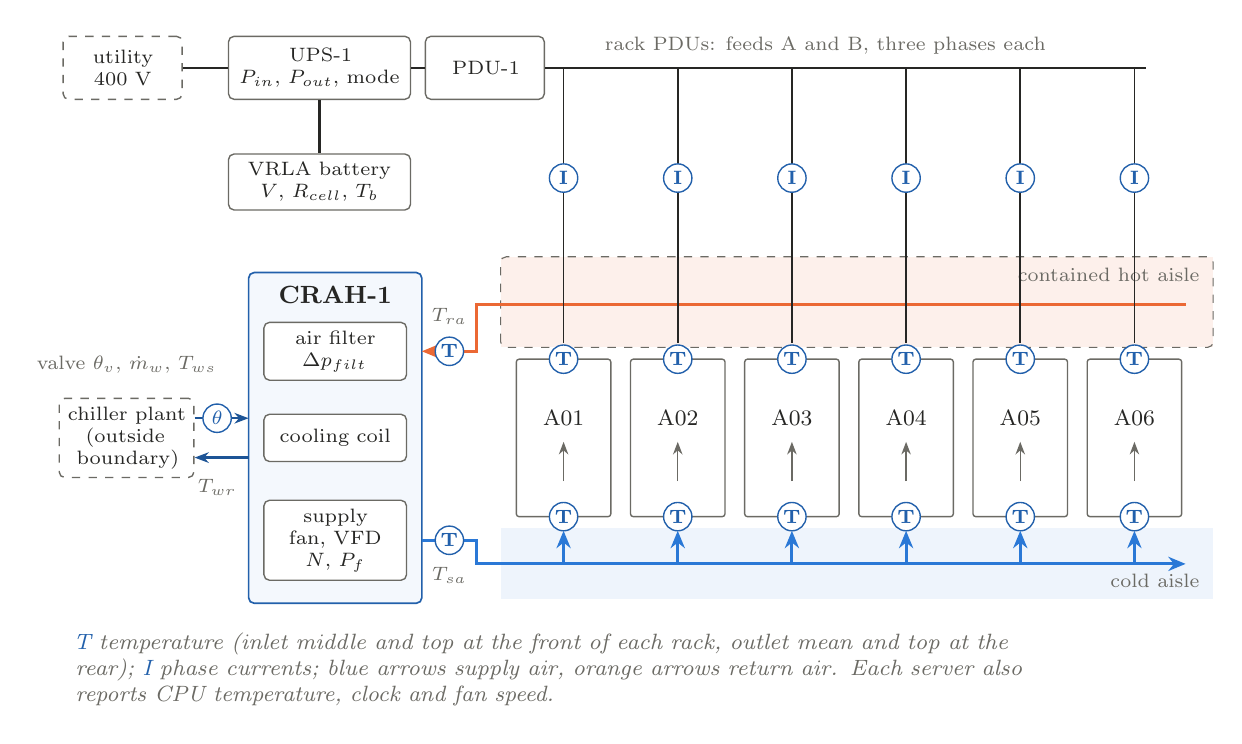
\begin{tikzpicture}[x=1cm, y=1cm]
  % ---- aisles (drawn first so everything else sits on top)
  \fill[accBlue!8] (3.2,0.25) rectangle (12.25,1.15);
  \fill[accOrange!10] (3.2,3.45) rectangle (12.25,4.6);
  \draw[inkSoft, dashed, rounded corners=2pt] (3.2,3.45) rectangle (12.25,4.6);
  \node[tag, anchor=south east] at (12.2,0.27) {cold aisle};
  \node[tag, anchor=north east] at (12.2,4.58) {contained hot aisle};

  % ---- racks
  \foreach \i in {1,...,6} {
    \pgfmathsetmacro{\xa}{3.4 + (\i-1)*1.45}
    \pgfmathsetmacro{\xc}{\xa + 0.6}
    \draw[inkSoft, fill=white, line width=0.5pt, rounded corners=1pt] (\xa,1.3) rectangle ++(1.2,2.0);
    \node[font=\footnotesize, text=inkMain] at (\xc,2.55) {A0\i};
    \draw[-{Stealth[length=1.6mm]}, draw=inkSoft, line width=0.5pt] (\xc,1.75) -- (\xc,2.25);
    \node[sensor] at (\xc,1.3) {T};
    \node[sensor] at (\xc,3.3) {T};
    \draw[cold] (\xc,0.7) -- (\xc,1.12);
  }

  % ---- cooling unit
  \draw[accBlue!80!black, fill=accBlue!5, line width=0.6pt, rounded corners=2pt] (0,0.2) rectangle (2.2,4.4);
  \node[font=\small\bfseries, text=inkMain] at (1.1,4.12) {CRAH-1};
  \node[base, fill=white, text width=1.6cm, font=\scriptsize, minimum height=6mm] at (1.1,3.4) {air filter\\ $\Delta p_{filt}$};
  \node[base, fill=white, text width=1.6cm, font=\scriptsize, minimum height=6mm] at (1.1,2.3) {cooling coil};
  \node[base, fill=white, text width=1.6cm, font=\scriptsize, minimum height=6mm] at (1.1,1.0) {supply fan, VFD\\ $N$, $P_f$};

  % ---- air paths
  \draw[cold] (2.2,1.0) -- (2.9,1.0) |- (11.9,0.7);
  \draw[hot] (11.9,4.0) -- (2.9,4.0) |- (2.2,3.4);
  \node[sensor] at (2.55,1.0) {T};
  \node[tag, anchor=north] at (2.55,0.78) {$T_{sa}$};
  \node[sensor] at (2.55,3.4) {T};
  \node[tag, anchor=south] at (2.55,3.62) {$T_{ra}$};

  % ---- chilled water
  \node[ext=1.5cm, font=\scriptsize] (plant) at (-1.55,2.3) {chiller plant\\ (outside\\ boundary)};
  \draw[water] (plant.east |- 0,2.55) -- (0,2.55);
  \draw[water] (0,2.05) -- (plant.east |- 0,2.05);
  \node[sensor] at (-0.4,2.55) {$\theta$};
  \node[tag, anchor=south] at (-1.55,3.0) {valve $\theta_v$, $\dot m_w$, $T_{ws}$};
  \node[tag, anchor=north] at (-0.4,1.9) {$T_{wr}$};

  % ---- power path
  \node[ext=1.3cm, font=\scriptsize] (util) at (-1.6,7.0) {utility\\ 400 V};
  \node[base, fill=white, text width=2.1cm, font=\scriptsize] (ups) at (0.9,7.0) {UPS-1\\ $P_{in}$, $P_{out}$, mode};
  \node[base, fill=white, text width=2.1cm, font=\scriptsize, minimum height=6mm] (bat) at (0.9,5.55) {VRLA battery\\ $V$, $R_{cell}$, $T_b$};
  \node[base, fill=white, text width=1.3cm, font=\scriptsize] (pdu) at (3.0,7.0) {PDU-1};
  \draw[power] (util) -- (ups);
  \draw[power] (ups) -- (pdu);
  \draw[power] (ups) -- (bat);
  \draw[power] (pdu.east) -- (11.4,7.0);
  \foreach \i in {1,...,6} {
    \pgfmathsetmacro{\xc}{3.4 + (\i-1)*1.45 + 0.6}
    \draw[power, line width=0.6pt] (\xc,7.0) -- (\xc,3.5);
    \node[sensor] at (\xc,5.6) {I};
  }
  \node[tag, anchor=south west] at (4.4,7.05) {rack PDUs: feeds A and B, three phases each};

  % ---- key
  \node[note, anchor=north west, text width=12cm, align=left] at (-2.3,-0.05)
    {\textcolor{accBlue!80!black}{T}~temperature (inlet middle and top at the front of each rack, outlet mean and top at the rear);
     \textcolor{accBlue!80!black}{I}~phase currents; blue arrows supply air, orange arrows return air.
     Each server also reports CPU temperature, clock and fan speed.};
\end{tikzpicture}

  \caption{Plan view of the data centre row: cooling unit, contained hot aisle, power path and sensors.}
  \label{fig:system}
\end{figure}

\subsection{Energy and material flows}

Four flows connect the components:

\begin{itemize}
  \item \textbf{Electrical.} Utility power passes through UPS-1, PDU-1 and the rack PDUs to the servers. Almost all of the electrical energy that the servers draw ends up as heat.
  \item \textbf{Air.} CRAH-1 discharges supply air into the cold aisle. Server fans draw it through the servers into the contained hot aisle, from which it returns to CRAH-1 through the filter and cooling coil.
  \item \textbf{Water.} Chilled water from the plant passes through a modulating control valve and the coil, absorbs the heat and returns to the plant.
  \item \textbf{Heat.} Server heat is carried by the air, transferred to the chilled water at the coil and leaves the boundary. UPS and PDU losses add to the room load.
\end{itemize}

In steady state, the heat removed from the air must equal the IT power plus the fan heat. The same heat must also equal what the water absorbs. These two balances can be computed from independent sensors, which gives the analytical redundancy that later separates sensor faults from equipment faults \parencite{isermann2006}.

\subsection{Operating conditions and control}

The row operates between low, nominal and high load, corresponding to mean processor utilisations of about 10\%, 50\% and 90\% and row IT loads of 54, 78 and 102\,kW (Section~\ref{sec:maths}). Four control loops shape its behaviour:

\begin{itemize}
  \item the CRAH valve modulates water flow to hold a supply-air setpoint of 20\,\textdegree C;
  \item the CRAH fan speed follows the airflow demand of the servers;
  \item each server's management controller sets its own fan speed from its internal temperatures;
  \item the UPS runs in double conversion, on battery or on static bypass.
\end{itemize}

\subsection{Governing principles}

Table~\ref{tab:principles} summarises the physical principles that the diagnostic knowledge relies on. Sensible heat transfer and the first law of thermodynamics underpin the energy balances. The fan affinity laws predict fan power from fan speed \parencite{ashraehvac2020}. The effectiveness--NTU method describes the cooling coil \parencite{incropera2011}. On the electrical side, three-phase power and the continuous-load limit of branch circuits \parencite{nfpa702023} govern overloads, while rising internal resistance indicates fading battery capacity \parencite{ieee1188}. On the computing side, server power grows roughly linearly with utilisation \parencite{fan2007}, and processors throttle their clock when they approach their junction temperature limit.

\begin{table}[htbp]
  \centering
  \small
  \caption{Governing principles and their diagnostic use.}
  \label{tab:principles}
  \begin{tabular}{L{3.1cm}L{5.9cm}L{5.0cm}}
    \toprule
    Domain & Principle & Diagnostic use \\
    \midrule
    Heat transfer & Sensible heat: $Q = \dot m c_p \Delta T$ & Air-side and water-side heat flows \\
    Thermodynamics & First law over the row & Cross-checks between independent sensors \\
    Fluid mechanics & Fan affinity laws & Expected fan power at a given speed \\
    Fluid mechanics & Filter pressure drop grows with loading & Filter clogging \\
    Heat exchange & Effectiveness--NTU coil model & Coil capacity and valve behaviour \\
    Electrical & Three-phase power; 80\% continuous-load limit & Branch overload, rack power balance \\
    Electrochemistry & Internal resistance rises as capacity fades & Battery degradation \\
    Computing & Server power linear in utilisation; thermal throttling & Expected heat; consequences of faults \\
    \bottomrule
  \end{tabular}
\end{table}

\subsection{Normal and abnormal operation}

Table~\ref{tab:envelope} defines the normal operating envelope. Abnormal operation is any sustained departure from this envelope, or any break in the energy balances that exceeds the combined sensor uncertainty (Section~\ref{sec:balances}). Values marked as assumptions are design choices for the modelled row. They are justified where they are used, and their sensitivity is quantified in Chapter~\ref{ch:dataset_and_evaluation}.

\begin{table}[htbp]
  \centering
  \small
  \caption{Normal operating envelope of the row.}
  \label{tab:envelope}
  \begin{tabular}{L{5.4cm}L{4.4cm}L{4.2cm}}
    \toprule
    Variable & Normal range & Source \\
    \midrule
    Rack inlet temperature & 18 to 27\,\textdegree C (allowable 15 to 32\,\textdegree C, class A1) & \textcite{ashrae2021} \\
    Inlet stratification, top minus middle & below 3\,K & Assumption \\
    Supply-air temperature & 20\,\textdegree C $\pm$ 2\,K & Design setpoint \\
    Chilled-water temperature rise & about 5 to 7\,K & Design value \\
    Fan power over affinity-law prediction & 0.95 to 1.05 & Assumption \\
    Branch current & at most 80\% of breaker rating & \textcite{nfpa702023} \\
    UPS efficiency, double conversion & about 0.95 & Manufacturer data (to verify) \\
    VRLA float voltage & 2.25 to 2.30\,V per cell at 25\,\textdegree C & Manufacturer data (to verify) \\
    Cell internal resistance & within 15\% of commissioning baseline & Assumption, after \textcite{ieee1188} \\
    Telemetry sample age & below 60\,s & Assumption \\
    \bottomrule
  \end{tabular}
\end{table}

% ---------------------------------------------------------------------------
\section{Fault Mechanisms}
\label{sec:faults}

\subsection{Fault taxonomy}

The fault universe contains eight physical faults, two instrumentation faults and normal operation:
\begin{equation}
  \mathcal{F} = \{F_1, \dots, F_8, S_1, S_2, F_N\}.
\end{equation}
Each fault was admitted only if it is a recognised failure mode with a distinct observable signature inside the system boundary. No category was created merely to increase the number of classes. Physical faults ($F$) are kept separate from instrumentation faults ($S$), because a sensor fault calls for a different corrective action than an equipment fault. Table~\ref{tab:taxonomy} gives the physical meaning, causes, symptoms and consequences of each.

\begin{small}
\begin{longtable}{L{2.0cm}L{2.9cm}L{2.8cm}L{3.3cm}L{2.5cm}}
  \caption{Fault taxonomy.}\label{tab:taxonomy}\\
  \toprule
  Fault & Physical meaning & Typical causes & Observable symptoms & Consequences \\
  \midrule
  \endfirsthead
  \toprule
  Fault & Physical meaning & Typical causes & Observable symptoms & Consequences \\
  \midrule
  \endhead
  $F_N$ normal & All variables within the envelope; balances close & -- & Inlets 18 to 27\,\textdegree C; supply at setpoint; fan power matches speed & -- \\
  $F_1$ CRAH fan failure & Fan delivers little or no air at its commanded speed & Motor burnout, broken belt or coupling, drive trip & Fan power far below prediction; row-wide hot inlets; supply air colder than setpoint & Row overheating, throttling, shutdowns \\
  $F_2$ chilled-water loss & Coil receives too little water flow & Seized valve, plant pump trip, closed isolation valve, air lock & Water flow far below the valve prediction; supply air hot; fan healthy & Row overheating \\
  $F_3$ filter clogging & Filter resistance rises, cutting airflow at a given speed & Missed replacement, construction dust & High filter loading ratio; fan speed rising & Higher fan energy; leads towards $F_1$ \\
  $F_4$ hot-air recirculation & Hot exhaust re-enters the server inlets & Missing blanking panels, open containment doors & Top inlet and exhaust stratified on one rack; CRAH healthy & Local overheating of upper servers \\
  $F_5$ server fan failure & One server loses internal airflow & Fan wear, failed fan controller & Server fan speed near zero; CPU near 95\,\textdegree C; clock reduced & Throttling or shutdown of one server \\
  $F_6$ branch overload & A phase circuit exceeds its continuous rating & Added servers, peaks, phase imbalance & Phase current above 80\% of the breaker rating & Breaker trip dropping all servers on the circuit \\
  $F_7$ battery degradation & Capacity has faded, shortening ride-through & Age, heat, sulphation, dry-out & Cell resistance well above baseline; low float voltage & Load drop during a utility event \\
  $F_8$ UPS on bypass & UPS has transferred the load to static bypass & Inverter or rectifier fault, overload & Mode flag shows bypass; efficiency about 1.0 & No battery protection \\
  $S_1$ sensor bias & A temperature sensor reads offset from the truth & Drift, poor placement, loose mounting & One sensor disagrees with neighbours and with the energy balance & False alarms or a masked fault \\
  $S_2$ telemetry dropout & Readings are stale or missing & Agent crash, network loss & Sample age above the limit & Incomplete evidence \\
  \bottomrule
\end{longtable}
\end{small}

Several pairs of faults share symptoms, and the observation vector was chosen to separate them. $F_1$ and $F_2$ both overheat the whole row. They differ in fan power and in chilled-water flow measured against valve position. $F_3$ and $F_1$ are points on the same airflow-loss path, gradual and abrupt, but call for different actions. $F_4$ is local to a rack while the cooling unit is healthy, and $F_5$ is local to one server. $S_1$ can either imitate $F_4$, when a top inlet sensor reads high, or hide it, when the sensor reads low. Figure~\ref{fig:propagation} traces each fault from its mechanism to its observable effect and its consequence.

\begin{figure}[htbp]
  \centering
  % Figure 4: fault propagation and causal structure.
\begin{tikzpicture}[x=1cm, y=1cm]
  \node[grouplabel] at (1.5,0.75) {Fault};
  \node[grouplabel] at (5.3,0.75) {Mechanism};
  \node[grouplabel] at (9.1,0.75) {Observable effect};
  \node[grouplabel] at (12.9,0.75) {Consequence};

  \tikzset{f/.style={kb=2.9cm, font=\footnotesize, minimum height=7mm},
           m/.style={reason=2.9cm, font=\footnotesize, minimum height=7mm},
           e/.style={data=2.9cm, font=\footnotesize, minimum height=7mm},
           c/.style={out=2.9cm, font=\footnotesize, minimum height=7mm}}

  % cooling chain
  \node[f] (f3) at (1.5,0)    {F3 filter clogging};
  \node[f] (f1) at (1.5,-1.1) {F1 CRAH fan failure};
  \node[f] (f2) at (1.5,-2.2) {F2 chilled-water loss};
  \node[m] (m3) at (5.3,0)    {airflow reduced};
  \node[m] (m1) at (5.3,-1.1) {airflow lost};
  \node[m] (m2) at (5.3,-2.2) {coil cannot absorb heat};
  \node[e] (e1) at (9.1,-1.1) {row inlets above 27\,\textdegree C};
  % rack and server
  \node[f] (f4) at (1.5,-3.5) {F4 hot-air recirculation};
  \node[m] (m4) at (5.3,-3.5) {exhaust re-enters the inlets};
  \node[e] (e4) at (9.1,-3.5) {top inlet and exhaust stratified};
  \node[f] (f5) at (1.5,-4.6) {F5 server fan failure};
  \node[m] (m5) at (5.3,-4.6) {server airflow lost};
  \node[e] (e5) at (9.1,-4.6) {CPU near 95\,\textdegree C};
  \node[c] (c1) at (12.9,-2.8) {CPU throttling and server shutdown};
  % power
  \node[f] (f6) at (1.5,-5.9) {F6 branch overload};
  \node[m] (m6) at (5.3,-5.9) {current above 80\% of rating};
  \node[e] (e6) at (9.1,-5.9) {breaker trip};
  \node[f] (f7) at (1.5,-7.0) {F7 battery degradation};
  \node[m] (m7) at (5.3,-7.0) {capacity fades};
  \node[f] (f8) at (1.5,-8.1) {F8 UPS on bypass};
  \node[m] (m8) at (5.3,-8.1) {no battery path};
  \node[e] (e7) at (9.1,-7.55) {no ride-through on a utility event};
  \node[c] (c2) at (12.9,-6.7) {servers lose power};
  % instrumentation
  \node[f] (s1) at (1.5,-9.4) {S1 sensor bias};
  \node[m] (ms1) at (5.3,-9.4) {false or hidden reading, can mask F4};
  \node[f] (s2) at (1.5,-10.5) {S2 telemetry dropout};
  \node[m] (ms2) at (5.3,-10.5) {stale data};
  \node[c] (c3) at (12.9,-9.95) {wrong, missed or uncertain diagnosis};

  \foreach \a/\b in {f3/m3, f1/m1, f2/m2, f4/m4, m4/e4, f5/m5, m5/e5, f6/m6, m6/e6, f7/m7, f8/m8, s1/ms1, s2/ms2}
    \draw[flow] (\a) -- (\b);
  \draw[flow] (m3.east) -- ++(0.4,0) |- (e1.west);
  \draw[flow] (m1) -- (e1);
  \draw[flow] (m2.east) -- ++(0.4,0) |- (e1.west);
  \draw[flow] (e1.east) -- ++(0.4,0) |- (c1.west);
  \draw[flow] (e4.east) -- ++(0.4,0) |- (c1.west);
  \draw[flow] (e5.east) -- ++(0.4,0) |- (c1.west);
  \draw[flow] (m7.east) -- ++(0.4,0) |- (e7.west);
  \draw[flow] (m8.east) -- ++(0.4,0) |- (e7.west);
  \draw[flow] (e6.east) -- ++(0.4,0) |- (c2.west);
  \draw[flow] (e7.east) -- ++(0.4,0) |- (c2.west);
  \draw[flow] (ms1.east) -- ++(0.6,0) |- (c3.west);
  \draw[flow] (ms2.east) -- ++(0.6,0) |- (c3.west);
  \draw[feedback] (f3.west) -- ++(-0.3,0) |- node[tag, pos=0.25, rotate=90, anchor=south] {worsens} (f1.west);
\end{tikzpicture}

  \caption{Fault propagation: how each fault in the taxonomy leads to observable effects and consequences.}
  \label{fig:propagation}
\end{figure}

\subsection{Multiple and interacting faults}

Faults can occur together and interact. Five combinations are used in the multiple-fault tests (Table~\ref{tab:interactions}). They were chosen because each tests a distinct interaction: aggravation, masking, compound risk and co-location.

\begin{table}[htbp]
  \centering
  \small
  \caption{Interacting faults used in the multiple-fault tests.}
  \label{tab:interactions}
  \begin{tabular}{L{3.2cm}L{10.8cm}}
    \toprule
    Combination & Interaction \\
    \midrule
    $F_3$ with $F_4$ & Reduced airflow aggravates recirculation at a leaky rack. \\
    $F_4$ with $S_1$ & A low-reading top inlet sensor hides a real recirculation hot spot. \\
    $F_7$ with $F_8$ & The load sits on bypass while the battery is weak, a compound risk to continuity. \\
    $F_1$ with $F_6$ & A cooling and an electrical fault occur together and must both be reported. \\
    $F_4$ with $F_5$ & A failed server fan inside a recirculating rack. \\
    \bottomrule
  \end{tabular}
\end{table}

% ---------------------------------------------------------------------------
\section{Foundations of Knowledge Representation and Reasoning}
\label{sec:krr}

Knowledge representation and reasoning studies how knowledge can be written in a formal language so that a program can draw conclusions from it that are justified by the knowledge alone \parencite{brachman2004}. Two properties matter most for engineering diagnosis. The representation must be \emph{declarative}, so that each piece of knowledge has a meaning independent of how it is used. The reasoning must be \emph{sound} with respect to that meaning, so that every conclusion can be justified by tracing it back to the knowledge and the observations that support it.

\subsection{Logic programming and Horn clauses}

Logic programming represents knowledge as definite clauses, also called Horn clauses, of the form $H \leftarrow B_1 \wedge \dots \wedge B_n$: the head $H$ holds whenever every body literal $B_i$ holds \parencite{kowalski1979,lloyd1987}. A set of such clauses has a least Herbrand model, and SLD resolution derives exactly the ground atoms that are true in it, so the procedural reading of a Prolog program coincides with its logical reading for this fragment \parencite{lloyd1987}. Prolog adds arithmetic, built-in predicates and a fixed left-to-right, depth-first search strategy \parencite{bratko2012}.

\subsection{Negation as failure and the closed-world assumption}

Diagnosis needs negative conclusions, such as ``the supply air is \emph{not} hot'' or ``no fault rule fires''. Prolog provides negation as failure: $\neg G$ succeeds when every attempt to prove $G$ fails. Under the closed-world assumption, whatever cannot be derived is taken to be false, and \textcite{clark1978} showed that negation as failure is sound with respect to the completion of the program. This project uses negation as failure in two controlled places: to conclude normal operation when no fault rule fires and every inlet is within the envelope, and to block a rule when contrary evidence can be proved. Section~\ref{sec:kr-scheme} explains why missing evidence is never treated as negative evidence in the model-based modules, which would otherwise make the closed-world assumption dangerous.

\subsection{Expert systems and explanation}

An expert system separates a knowledge base, written by or with domain experts, from an inference engine that applies it \parencite{jackson1998}. Its defining requirement is transparency: it must be able to say why it reached a conclusion and which knowledge it used. Rule-based systems meet this naturally, because every conclusion is the head of a rule whose body was proved. This project keeps that property for all three reasoning modes by recording the proof of every deductive conclusion, the evidence behind every abductive hypothesis and the conflict sets behind every consistency-based diagnosis (Chapter~\ref{ch:design_and_development}).

% ---------------------------------------------------------------------------
\section{Knowledge Representation Scheme}
\label{sec:kr-scheme}

\subsection{Observation vector}

The observation vector is $\mathbf{x} = [x_1, x_2, \dots, x_{26}]^{\mathsf T}$. Every variable that appears in an equation, a table, a figure or a Prolog predicate is defined in Table~\ref{tab:variables}. Each observation is stored as a fact \texttt{obs(Case, Variable, Entity, Value)}. Entities are named systematically: racks \texttt{rack\_a01} to \texttt{rack\_a06}, servers \texttt{rack\_a01\_s01} onwards, rack PDU phases \texttt{rack\_a01\_a\_l1} onwards, and \texttt{crah\_1}, \texttt{ups\_1} and \texttt{battery\_1}.

\begin{small}
\begin{longtable}{L{1.2cm}L{4.3cm}L{1.2cm}L{3.1cm}L{3.9cm}}
  \caption{Observation variables.}\label{tab:variables}\\
  \toprule
  Symbol & Variable & Unit & Prolog name & Diagnostic relevance \\
  \midrule
  \endfirsthead
  \toprule
  Symbol & Variable & Unit & Prolog name & Diagnostic relevance \\
  \midrule
  \endhead
  $x_1$ & Rack inlet temperature, middle & \textdegree C & \texttt{t\_inlet\_mid} & Envelope; neighbour consistency \\
  $x_2$ & Rack inlet temperature, top & \textdegree C & \texttt{t\_inlet\_top} & Stratification ($F_4$, $S_1$) \\
  $x_3$ & Rack outlet temperature, mean & \textdegree C & \texttt{t\_outlet} & Outlet stratification \\
  $x_4$ & CRAH supply-air temperature & \textdegree C & \texttt{t\_supply\_air} & $F_1$, $F_2$, $S_1$ \\
  $x_5$ & CRAH return-air temperature & \textdegree C & \texttt{t\_return\_air} & Air-side balance \\
  $x_6$ & CRAH fan speed & \% & \texttt{fan\_speed} & Affinity-law prediction \\
  $x_7$ & CRAH fan electrical power & kW & \texttt{fan\_power} & $F_1$ \\
  $x_8$ & Filter differential pressure & Pa & \texttt{dp\_filter} & $F_3$ \\
  $x_9$ & Chilled-water supply temperature & \textdegree C & \texttt{t\_chw\_supply} & Water-side balance \\
  $x_{10}$ & Chilled-water return temperature & \textdegree C & \texttt{t\_chw\_return} & Water-side balance \\
  $x_{11}$ & Chilled-water valve position & \% & \texttt{valve\_position} & Valve prediction ($F_2$) \\
  $x_{12}$ & Rack PDU phase current & A & \texttt{i\_branch} & $F_6$; power balance \\
  $x_{13}$ & Rack IT power & kW & \texttt{p\_rack} & Power balance \\
  $x_{14}$ & Mean CPU utilisation of a rack & -- & \texttt{cpu\_util} & Expected heat \\
  $x_{15}$ & Server CPU temperature & \textdegree C & \texttt{t\_cpu} & $F_5$ \\
  $x_{16}$ & Server CPU clock frequency & GHz & \texttt{f\_cpu} & Throttling \\
  $x_{17}$ & Server fan speed & rpm & \texttt{server\_fan\_rpm} & $F_5$ \\
  $x_{18}$ & UPS input power & kW & \texttt{p\_ups\_in} & UPS efficiency ($F_8$) \\
  $x_{19}$ & UPS output power & kW & \texttt{p\_ups\_out} & UPS efficiency ($F_8$) \\
  $x_{20}$ & UPS operating mode & -- & \texttt{ups\_mode} & $F_8$ \\
  $x_{21}$ & Battery string float voltage & V & \texttt{v\_battery} & $F_7$ \\
  $x_{22}$ & Highest cell internal resistance & m$\Omega$ & \texttt{r\_cell} & $F_7$ \\
  $x_{23}$ & Battery temperature & \textdegree C & \texttt{t\_battery} & Ageing \\
  $x_{24}$ & Telemetry sample age & s & \texttt{sample\_age} & $S_2$ \\
  $x_{25}$ & Chilled-water mass flow & kg/s & \texttt{m\_chw} & $F_2$; water-side balance \\
  $x_{26}$ & Rack outlet temperature, top & \textdegree C & \texttt{t\_outlet\_top} & Outlet stratification \\
  \bottomrule
\end{longtable}
\end{small}

\subsection{Layers of the knowledge base}

The knowledge base is organised in seven layers, each a set of Prolog facts or Horn clauses. Table~\ref{tab:kr-layers} lists them. Two design choices deserve explanation.

\paragraph{Rules as data.} Diagnostic rules are stored as facts \texttt{drule(Id, Head, Body, Source)} rather than as ordinary clauses. A small meta-interpreter proves them and returns a proof tree for every conclusion. Each rule remains a Horn clause, $\textit{Head} \leftarrow \textit{Body}$, so the logical reading is unchanged. Storing rules as data gives every rule an identifier and a source, which the explanation facility reports, and lets the rule table in the report be generated directly from the knowledge base.

\paragraph{Provenance on every threshold and rule.} Every threshold fact (\texttt{threshold/4}) and every rule names a source fact (\texttt{source/3}), whose type is \texttt{standard}, \texttt{literature}, \texttt{assumption} or \texttt{method}. This keeps four kinds of information apart, as the project framework requires: measured data (none in this project), synthetic test cases, engineering assumptions and literature-supported rules.

\begin{table}[htbp]
  \centering
  \small
  \caption{Layers of the knowledge base.}
  \label{tab:kr-layers}
  \begin{tabular}{L{3.4cm}L{4.6cm}L{6.0cm}}
    \toprule
    Layer & Representation & Content \\
    \midrule
    Structure & \texttt{component/2}, \texttt{serves/2}, \texttt{rated/4} & Components, topology and ratings \\
    Reference values & \texttt{threshold/4}, \texttt{source/3} & Envelopes and limits with provenance \\
    Engineering calculations & Horn clauses with arithmetic & The equations of Section~\ref{sec:maths} \\
    Diagnostic rules & \texttt{drule/4} & 47 rules deriving conditions and faults \\
    Causal knowledge & \texttt{evidence/3}, \texttt{requires/2}, \texttt{masks/2} & Fault signatures for abduction \\
    Redundancy relations & \texttt{arr/3}, \texttt{fm/2} & Relations, support sets and fault models \\
    Maintenance knowledge & \texttt{maintenance/5}, \texttt{plan\_interaction/3} & Corrective plans and their ordering \\
    \bottomrule
  \end{tabular}
\end{table}

\subsection{Graded evidence and the open-world treatment of missing data}

The deductive rules compare features with crisp thresholds. The abductive and consistency-based modules instead use graded symptoms. Each symptom receives an evidence strength between 0 and 1, scaled to the measurement noise estimated from the case itself (Equations~\eqref{eq:grade} and~\eqref{eq:sigma}), and a status of present, absent, uncertain or unknown. A symptom whose inputs are missing is \emph{unknown}, never absent. The closed-world assumption is therefore applied only where it is safe: in the deductive rules, and in the final ``normal'' conclusion. It is never used to infer that a symptom is absent merely because it could not be computed.

% ---------------------------------------------------------------------------
\section{Diagnosis Theory: Deductive, Abductive and Consistency-Based}
\label{sec:diagnosis-theory}

Let $\mathit{KB}$ be the knowledge base and $E$ the evidence: the observations of a case together with the conditions derived from them. Three theories of diagnosis are implemented. \textcite{console1991} show that they are points on one spectrum of logical definitions of model-based diagnosis.

\paragraph{Deductive diagnosis.} A fault $F_k$ is diagnosed when it follows from the knowledge base and the evidence:
\begin{equation}
  \mathit{KB} \cup E \models F_k .
  \label{eq:deductive}
\end{equation}
This is the classical reading of a rule-based expert system. It is efficient and transparent, but it needs a rule for every symptom pattern, and a crisp rule turns measurement noise directly into false findings.

\paragraph{Abductive diagnosis.} Abduction reasons from effects to causes. A set of hypotheses $D \subseteq \mathcal{H}$, where $\mathcal{H} = \mathcal{F} \setminus \{F_N\}$, is an explanation when it entails the evidence and is consistent with it \parencite{poole1989}:
\begin{equation}
  D \cup \mathit{KB} \models E, \qquad D \cup \mathit{KB} \cup E \not\models \bot .
  \label{eq:abductive}
\end{equation}
Among the explanations, the parsimony principle prefers the smallest:
\begin{equation}
  D^{*} = \arg\min_{D} \lvert D \rvert .
  \label{eq:parsimony}
\end{equation}
The implementation follows parsimonious covering theory \parencite{peng1990}: causal knowledge states which symptoms each fault can explain, and the search finds minimal sets of faults that cover every clearly present symptom.

\paragraph{Consistency-based diagnosis.} Consistency-based diagnosis reasons from a model of correct behaviour \parencite{reiter1987,dekleer1987}. Let $\mathit{SD}$ be the system description, $\mathit{COMPS}$ the set of components, $\mathit{OBS}$ the observations and $\mathit{AB}(c)$ the statement that component $c$ is abnormal. A set $\Delta \subseteq \mathit{COMPS}$ is a diagnosis when
\begin{equation}
  \mathit{SD} \cup \mathit{OBS} \cup \{\mathit{AB}(c) \mid c \in \Delta\} \cup \{\neg\mathit{AB}(c) \mid c \in \mathit{COMPS} \setminus \Delta\} \not\models \bot .
  \label{eq:reiter}
\end{equation}
A conflict set is a set of components that cannot all be healthy given the observations. \textcite{reiter1987} proved that the minimal diagnoses are exactly the minimal hitting sets of the conflict sets. In this project the behaviour model is written as analytical redundancy relations, each of which holds when a named set of components is healthy, which links consistency-based diagnosis to the fault detection practice of control engineering \parencite{cordier2004}. Sensors are treated as components, so a sensor fault is a diagnosis like any other. Pure consistency-based diagnosis cannot exonerate a component, because it never predicts what a fault would look like. Fault models remove this limitation \parencite{struss1989}: if a component is abnormal, a named relation must also be violated, so a component whose fault model predicts a violation that clearly did not happen is exonerated.

\paragraph{Combining the three.} The complete system combines the modes as ``abduction proposes, consistency disposes''. Abduction produces ranked candidate explanations, and the best-ranked one that is also a consistent diagnosis in the sense of Equation~\eqref{eq:reiter} is accepted. Chapter~\ref{ch:design_and_development} describes the implementation, and Chapter~\ref{ch:dataset_and_evaluation} compares the four configurations that the framework asks for.

% ---------------------------------------------------------------------------
\section{Mathematical Formulation}
\label{sec:maths}

This section gives the engineering and logical model in full. Equations carry the tags E1 to E56 used in the design documents and in the comments of \texttt{kb/calculations.pl}, so that each equation can be traced to the predicate that implements it. Equations with a letter suffix, such as E11a, were added during development. Every symbol is defined where it first appears and again in Table~\ref{tab:nomenclature}.

\subsection{Sets and indices}

$\mathcal{R} = \{r_1, \dots, r_6\}$ is the set of racks, with $n_R = \lvert\mathcal{R}\rvert = 6$. $\mathcal{S}_r$ is the set of servers in rack $r$, with $\lvert\mathcal{S}_r\rvert = 20$.

\subsection{IT power}

Server power is close to linear in CPU utilisation $u_s \in [0,1]$ \parencite{fan2007}:
\begin{align}
  P_s &= P_{idle} + (P_{max} - P_{idle})\, u_s , \tag{E1}\label{eq:e1}\\
  P_r &= \textstyle\sum_{s \in \mathcal{S}_r} P_s , \tag{E2}\\
  P_{IT} &= \textstyle\sum_{r \in \mathcal{R}} P_r , \tag{E3}\\
  \varepsilon_{P,r} &= \frac{P_r^{meas} - P_r}{P_r} . \tag{E4}
\end{align}
With $P_{idle} = 0.40$\,kW and $P_{max} = 0.90$\,kW per server, utilisations of 10\%, 50\% and 90\% give row loads of 54, 78 and 102\,kW. $P_r^{meas}$ is the metered rack power and $\varepsilon_{P,r}$ the model residual.

\subsection{Server and rack thermal model}

\begin{align}
  \dot m &= \rho_a \dot V , \tag{E5}\\
  \Delta T_s &= \frac{P_s}{\dot m_s\, c_{p,a}} , \tag{E6}\\
  T_{out,r} &= T_{in,r} + \frac{P_r}{\dot m_r\, c_{p,a}} , \tag{E7}\\
  T_{cpu,s} &= T_{in,r} + R_{th}(\omega_s)\, P_{cpu,s} , \tag{E8}\\
  \phi_{f,s} &= f_{cpu,s} / f_{nom,s} . \tag{E9}
\end{align}
$\dot m$ is mass flow, $\rho_a$ air density, $\dot V$ volume flow and $c_{p,a}$ the specific heat of air. Equation E6 gives a rise of about 13\,K across a server at nominal load. In E8, the junction-to-inlet thermal resistance $R_{th}$ rises as the server fan speed $\omega_s$ falls, so a failed server fan ($F_5$) raises the CPU temperature even when the inlet is normal. A frequency ratio $\phi_{f,s} < 1$ shows throttling, which is a consequence of $F_1$, $F_2$, $F_4$ or $F_5$ and not a fault class of its own.

\subsection{Rack inlet indicators}

\begin{align}
  T_{in,max,r} &= \max(T_{in,top,r},\, T_{in,mid,r}) , \tag{E10}\\
  \Delta T_{strat,r} &= T_{in,top,r} - T_{in,mid,r} , \tag{E11}\\
  \Delta T_{strat,out,r} &= T_{out,top,r} - T_{out,bot,r} = 2\,(T_{out,top,r} - T_{out,r}) , \tag{E11a}\label{eq:e11a}\\
  h_r &= \mathbf{1}\!\left[T_{in,max,r} > T_{rec,max}\right] , \tag{E12}\\
  \phi_{hot} &= \frac{1}{n_R} \textstyle\sum_{r} h_r . \tag{E13}
\end{align}
$\mathbf{1}[\cdot]$ is 1 when its condition holds and 0 otherwise, and $T_{rec,max} = 27$\,\textdegree C \parencite{ashrae2021}. A hot-rack fraction $\phi_{hot} \ge 0.5$ points to a row-level cause such as $F_1$ or $F_2$; a smaller fraction points to a rack-level cause such as $F_4$. Equation E11a assumes that the two halves of a rack carry similar airflow, so the lower-half outlet temperature is $2T_{out,r} - T_{out,top,r}$. Real recirculation heats the upper servers' inlet air, so their exhaust becomes hotter too and E11a rises with E11. A biased top inlet sensor changes E11 but not E11a, which is how $F_4$ is separated from $S_1$.

The supply and return heat indices \parencite{sharma2002} and the rack cooling indices \parencite{herrlin2005} summarise the thermal health of the row:
\begin{align}
  \mathit{SHI} &= \frac{\sum_r (T_{in,r} - T_{sa})}{\sum_r (T_{out,r} - T_{sa})} , \qquad \mathit{RHI} = 1 - \mathit{SHI} , \tag{E14--E15}\\
  \mathit{RCI}_{HI} &= \left[1 - \frac{\sum_r (T_{in,r} - T_{rec,max})\,\mathbf{1}[T_{in,r} > T_{rec,max}]}{n_R\,(T_{all,max} - T_{rec,max})}\right] \times 100\% , \tag{E16}\\
  \mathit{RCI}_{LO} &= \left[1 - \frac{\sum_r (T_{rec,min} - T_{in,r})\,\mathbf{1}[T_{in,r} < T_{rec,min}]}{n_R\,(T_{rec,min} - T_{all,min})}\right] \times 100\% . \tag{E17}
\end{align}
The mixing model behind $F_4$ treats the air at an inlet as a blend of supply air and exhaust, with recirculation fraction $\beta_r \in [0,1]$:
\begin{equation}
  T_{in,r} = (1 - \beta_r)\, T_{sa} + \beta_r\, T_{out,r} , \qquad
  \beta_r = \frac{T_{in,r} - T_{sa}}{T_{out,r} - T_{sa}} . \tag{E18--E19}\label{eq:mixing}
\end{equation}
Because $\beta_r \ge 0$ and $T_{out,r} > T_{sa}$, the mixing model implies that a top inlet can never be colder than the middle inlet. A top sensor that reads colder must therefore be faulty.

\subsection{CRAH air side and fan}

\begin{align}
  Q_a &= \dot m_a\, c_{p,a}\, (T_{ra} - T_{sa}) , \tag{E20}\\
  \dot V_a &= \dot V_{rated}\,(N / N_{rated}) , \tag{E21}\\
  \Delta p_{fan} &= \Delta p_{rated}\,(N / N_{rated})^2 , \tag{E22}\\
  P_{f,exp} &= P_{f,rated}\,(N / N_{rated})^3 , \tag{E23}\\
  \rho_f &= P_f / P_{f,exp} , \tag{E24}\\
  P_f &= \dot V_a\, \Delta p_{tot} / \eta_f , \tag{E25}\\
  \Delta p_{filt} &= K_{filt}\, \dot V_a^2 , \tag{E26}\\
  \lambda_{filt} &= \frac{\Delta p_{filt} / \dot V_a^2}{K_{filt,clean}} , \tag{E27}\\
  \delta_{sa} &= T_{sa} - T_{sp} . \tag{E28}
\end{align}
Equations E21 to E23 are the fan affinity laws \parencite{ashraehvac2020}. A healthy fan has a power ratio $\rho_f$ within about 5\% of 1. A ratio below 0.85 shows a partial failure such as belt slip, and below 0.5 a fan that is not moving air at all ($F_1$). The filter loading ratio $\lambda_{filt}$ normalises the filter resistance by its clean value, so it does not depend on fan speed; values well above 1 indicate $F_3$. A negative supply-air deviation $\delta_{sa}$ with row-wide overheating supports $F_1$, because the coil over-cools the small airflow that remains.

\subsection{Chilled-water side and coil}

\begin{align}
  \Delta T_w &= T_{wr} - T_{ws} , \tag{E29}\\
  Q_w &= \dot m_w\, c_{p,w}\, \Delta T_w , \tag{E30}\\
  Q_{coil} &= \varepsilon\, C_{min}\, (T_{ra} - T_{ws}) , \tag{E31}\\
  \mathit{NTU} &= \frac{UA}{C_{min}} , \qquad C^{*} = \frac{C_{min}}{C_{max}} , \tag{E32}\\
  \varepsilon &= \frac{1 - \exp[-\mathit{NTU}(1 - C^{*})]}{1 - C^{*}\exp[-\mathit{NTU}(1 - C^{*})]} , \tag{E33}\\
  \dot m_w^{exp} &= \dot m_{w,max}\, \mathcal{R}_v^{\,\theta_v - 1} , \tag{E34}\\
  \rho_w &= \dot m_w^{meas} / \dot m_w^{exp} . \tag{E34a}
\end{align}
Equations E31 to E33 are the effectiveness--NTU model of the coil in counterflow form \parencite{incropera2011}, where $C = \dot m c_p$ is a heat capacity rate. Equation E34 is the characteristic of an equal-percentage valve with rangeability $\mathcal{R}_v$ and opening fraction $\theta_v$. The ratio $\rho_w$ compares measured flow with the flow the valve opening predicts. A ratio far below 1 with the valve open is the signature of $F_2$. The water temperature rise $\Delta T_w$ is \emph{not} a reliable signature of $F_2$: low flow makes it larger, not smaller. An earlier version of the knowledge base assumed the opposite, and Section~\ref{sec:acquisition} describes how the simulator exposed the error.

\subsection{Energy balances and analytical redundancy}
\label{sec:balances}

\begin{align}
  Q_a &= P_{IT} + P_f + Q_{env} , \tag{E35}\\
  Q_w &= Q_a , \tag{E36}\\
  r_1 &= \frac{Q_a - (P_{IT} + P_f)}{P_{IT}} , \tag{E37}\\
  r_2 &= \frac{Q_w - Q_a}{Q_a} . \tag{E38}
\end{align}
Equation E35 is the first law over the row, with fan heat in the airstream and a small envelope gain $Q_{env}$. Equation E36 states that the coil is adiabatic. A residual counts as violated only when it exceeds what sensor uncertainty can explain. For a product $Q = \dot m c_p \Delta T$, first-order propagation gives
\begin{equation}
  \frac{u_Q}{Q} = \sqrt{\left(\frac{u_{\dot m}}{\dot m}\right)^{2} + \left(\frac{\sqrt{2}\,u_T}{\Delta T}\right)^{2}} , \qquad
  \lvert r_i \rvert > \vartheta_i = k_c\, u_{r_i} , \tag{E39--E40}\label{eq:uncertainty}
\end{equation}
where $u$ denotes a standard uncertainty and $k_c$ a coverage factor. With the sensor accuracies of the modelled row, $u_{r_2} \approx 0.07$. The knowledge base uses $\vartheta_2 = 0.2$, close to $k_c = 3$, because chilled-water loss alone can produce $\lvert r_2 \rvert \approx 0.14$.

Two neighbour-consistency relations check individual temperature sensors against sensors that see the same air:
\begin{align}
  r_{S,r} &= T_{in,r} - \operatorname{median}_{j \in \mathcal{N}(r)} T_{in,j} , \tag{E41}\\
  r_{sa} &= T_{sa} - \operatorname{median}_{r \in \mathcal{R}} T_{in,mid,r} . \tag{E41a}
\end{align}
A large $r_{sa}$ can come from a biased supply-air sensor or from a real airflow shortfall, which warms the inlets with room and hot-aisle air. The two are separated by recomputing E38 with the supply-air reading replaced by the median middle inlet:
\begin{equation}
  r_2' = \frac{Q_w - \rho_a \dot V_a c_{p,a}\,(T_{ra} - \operatorname{median}_r T_{in,mid,r})}{\rho_a \dot V_a c_{p,a}\,(T_{ra} - \operatorname{median}_r T_{in,mid,r})} . \tag{E41b}\label{eq:e41b}
\end{equation}
If the sensor is biased, the substitution removes the error and $\lvert r_2' \rvert$ falls within the threshold. If airflow is really lost, the estimated airflow is still wrong and the balance stays broken. The sensor-fault hypothesis is accepted only if assuming it restores consistency, which is consistency-based reasoning applied to a single hypothesis.

\subsection{Electrical distribution and battery}

\begin{align}
  P &= \sqrt{3}\, V_{LL}\, I \cos\varphi , \tag{E42}\\
  L_b &= I_b / I_{brk,b} , \tag{E43}\\
  \mathit{IU} &= \frac{\max_{p} \lvert I_p - \bar I \rvert}{\bar I} , \tag{E44}\\
  \eta_{UPS} &= P_{UPS,out} / P_{UPS,in} , \qquad P_{UPS,loss} = P_{UPS,in} - P_{UPS,out} , \tag{E45--E46}\\
  \mathit{pPUE} &= \frac{P_{IT} + P_f + P_{UPS,loss}}{P_{IT}} , \tag{E47}\\
  V_{cell} &= V_{str} / n_{cell} , \qquad \rho_R = R_{cell} / R_{cell,0} , \tag{E48--E49}\\
  t_{run} &= H \left(\frac{C_H}{I_{dis}\, H}\right)^{k_p} , \tag{E50}\\
  \mathcal{L}(T_b) &= \mathcal{L}_{25} \cdot 2^{-(T_b - 25)/10} . \tag{E51}
\end{align}
A branch loading ratio $L_b$ above 0.8 is an overload ($F_6$) under the continuous-load rule \parencite{nfpa702023}. Phase imbalance $\mathit{IU}$ is a common root cause. On static bypass ($F_8$), the UPS passes utility power straight through and $\eta_{UPS}$ rises from about 0.95 to about 1. Each rack's metered power should also equal the sum of its six phase powers, computed with E42 per phase. That relation separates a real overload from a faulty current sensor. A cell resistance ratio $\rho_R$ well above 1 indicates battery degradation ($F_7$) \parencite{ieee1188}. Equation E50 is Peukert's law for runtime, and E51 the common rule of thumb that VRLA life halves for every 10\,K above 25\,\textdegree C; both constants are to be confirmed against manufacturer data.

\subsection{Evidence, noise estimation and ranking}

\begin{align}
  a_x &= t_{now} - t_x , \tag{E52}\\
  \delta_x &= \frac{x - x_{ref}}{x_{ref}} , \qquad z_x = \frac{x - \mu_x}{\sigma_x} , \tag{E53}\label{eq:sigma}\\
  \hat x_k &= \alpha\, x_k + (1 - \alpha)\, \hat x_{k-1} , \tag{E54}\\
  e_j &= \min\!\left(1, \max\!\left(0,\ \tfrac{1}{2} + \frac{d_j}{4\sigma_j}\right)\right) , \tag{E55}\label{eq:grade}\\
  E_k &= \textstyle\sum_j w_{jk}\, e_j , \qquad \mathrm{Conf}(k) = \frac{E_k}{E_k + E_{\neg k} + \epsilon} . \tag{E56}
\end{align}
A sample older than 60\,s is stale ($S_2$). In E55, $d_j$ is the signed distance of a feature past its threshold and $\sigma_j$ its noise, so a symptom has evidence 0.5 exactly at its threshold and counts as present only one standard deviation beyond it. The noise is estimated from the case itself: the six middle inlets all see the same supply air, so their spread measures temperature-sensor noise. The robust estimate $\sigma_T = \max(0.15\,\mathrm{K},\ 1.4826\,\mathrm{MAD})$, using the median absolute deviation, cannot be distorted by one biased sensor \parencite{rousseeuw1993}. Electrical features use a noise scale estimated in the same way from the rack power balances. In E56, $w_{jk}$ is the weight of symptom $j$ for hypothesis $k$ and $E_{\neg k}$ the evidence against $k$ from expected symptoms that are clearly absent. $\mathrm{Conf}(k)$ ranks competing hypotheses. It is not a probability, and the model makes no probabilistic claim. Equation E54 is a noise filter for repeated readings and is not used, because each test case is a single snapshot.

\subsection{Closed-world normality and evaluation metrics}

Normal operation is concluded under the closed-world assumption when no fault can be derived and every inlet is within the envelope:
\begin{equation}
  F_N \iff \left(\forall F_k \in \mathcal{H}:\ \mathit{KB} \cup E \not\models F_k\right) \wedge \left(\forall r:\ T_{in,max,r} \le T_{rec,max}\right) .
\end{equation}
Performance is measured with the metrics required by the framework. With $\mathit{TP}$, $\mathit{TN}$, $\mathit{FP}$ and $\mathit{FN}$ the true and false positives and negatives of a fault class,
\begin{gather}
  \mathrm{Accuracy} = \frac{\mathit{TP} + \mathit{TN}}{\mathit{TP} + \mathit{TN} + \mathit{FP} + \mathit{FN}} , \quad
  \mathrm{Precision} = \frac{\mathit{TP}}{\mathit{TP} + \mathit{FP}} , \quad
  \mathrm{Recall} = \frac{\mathit{TP}}{\mathit{TP} + \mathit{FN}} , \label{eq:metrics} \\
  F_1 = \frac{2\,\mathrm{Precision}\cdot\mathrm{Recall}}{\mathrm{Precision} + \mathrm{Recall}} , \quad
  \mathrm{Coverage} = \frac{N_{correct}}{N_{test}} , \quad
  \mathrm{EMR} = \frac{1}{N_{test}} \textstyle\sum_i \mathbf{1}[\hat Y_i = Y_i] , \\
  \mathrm{ExplainabilityRate} = \frac{N_{valid\ explanations}}{N_{diagnoses}} , \qquad
  \mathrm{PlanValidity} = \frac{N_{valid\ plans}}{N_{plans}} ,
\end{gather}
where $Y_i$ and $\hat Y_i$ are the true and diagnosed fault sets of case $i$. Mean and maximum reasoning time complete the set. Chapter~\ref{ch:dataset_and_evaluation} defines exactly how each is counted for multiple-fault cases.

\begin{small}
\begin{longtable}{L{3.6cm}L{8.6cm}L{1.8cm}}
  \caption{Nomenclature.}\label{tab:nomenclature}\\
  \toprule
  Symbol & Meaning & Unit \\
  \midrule
  \endfirsthead
  \toprule
  Symbol & Meaning & Unit \\
  \midrule
  \endhead
  $a_x$ & Sample age of variable $x$ & s \\
  $C$, $C_{min}$, $C_{max}$, $C^{*}$ & Heat capacity rate $\dot m c_p$; smaller, larger; their ratio & kW/K \\
  $C_H$, $H$ & Battery rated capacity at rated discharge time $H$ & Ah, h \\
  $c_{p,a}$, $c_{p,w}$ & Specific heat of air (1.006) and water (4.186) & kJ/(kg\,K) \\
  $d_j$, $e_j$ & Distance past threshold; graded evidence of symptom $j$ & --, -- \\
  $E_k$, $E_{\neg k}$ & Weighted evidence for and against hypothesis $k$ & -- \\
  $f_{cpu,s}$, $f_{nom,s}$ & Measured and nominal CPU clock & GHz \\
  $h_r$ & Hot-rack indicator & -- \\
  $I$, $I_p$, $\bar I$, $I_b$, $I_{brk,b}$ & Line, phase and mean phase current; branch current and rating & A \\
  $I_{dis}$ & Battery discharge current & A \\
  $\mathit{IU}$ & Phase current imbalance & -- \\
  $K_{filt}$, $K_{filt,clean}$ & Filter resistance coefficient, current and clean & Pa\,s$^2$/m$^6$ \\
  $k_c$, $k_p$ & Coverage factor; Peukert exponent & -- \\
  $L_b$ & Branch loading ratio & -- \\
  $\mathcal{L}(T_b)$, $\mathcal{L}_{25}$ & Battery service life at $T_b$ and at 25\,\textdegree C & years \\
  $\dot m$, $\dot m_a$, $\dot m_r$, $\dot m_s$, $\dot m_w$ & Mass flow: general, CRAH air, rack, server, water & kg/s \\
  $\dot m_{w,max}$, $\dot m_w^{exp}$, $\dot m_w^{meas}$ & Water flow: valve fully open, predicted, measured & kg/s \\
  $N$, $N_{rated}$ & CRAH fan speed and rated speed & \% \\
  $n_R$, $n_{cell}$ & Number of racks; number of cells in series & -- \\
  $\mathit{NTU}$ & Number of transfer units & -- \\
  $P$, $P_s$, $P_r$, $P_{IT}$ & Three-phase power; server, rack and row IT power & kW \\
  $P_{idle}$, $P_{max}$, $P_{cpu,s}$ & Server idle and full-load power; CPU power & kW \\
  $P_f$, $P_{f,exp}$, $P_{f,rated}$ & Fan power: measured, expected, rated & kW \\
  $P_{UPS,in}$, $P_{UPS,out}$, $P_{UPS,loss}$ & UPS input, output and loss power & kW \\
  $\mathit{pPUE}$ & Partial power usage effectiveness of the row & -- \\
  $Q_a$, $Q_w$, $Q_{coil}$, $Q_{env}$ & Heat flows: air side, water side, coil, envelope & kW \\
  $R_{cell}$, $R_{cell,0}$ & Cell internal resistance, current and baseline & m$\Omega$ \\
  $R_{th}$ & CPU junction-to-inlet thermal resistance & K/kW \\
  $\mathcal{R}_v$ & Valve rangeability & -- \\
  $r_1$, $r_2$, $r_2'$ & Energy balance residuals; $r_2$ with substituted supply air & -- \\
  $r_{S,r}$, $r_{sa}$ & Neighbour-consistency residuals & K \\
  $\mathit{RCI}_{HI}$, $\mathit{RCI}_{LO}$ & Rack cooling indices & \% \\
  $\mathit{SHI}$, $\mathit{RHI}$ & Supply and return heat indices & -- \\
  $T_{in,r}$, $T_{in,top,r}$, $T_{in,mid,r}$, $T_{in,max,r}$ & Rack inlet temperature: general, top, middle, maximum & \textdegree C \\
  $T_{out,r}$, $T_{out,top,r}$, $T_{out,bot,r}$ & Rack outlet temperature: mean, upper half, lower half & \textdegree C \\
  $T_{sa}$, $T_{ra}$, $T_{sp}$ & CRAH supply, return and setpoint temperatures & \textdegree C \\
  $T_{ws}$, $T_{wr}$ & Chilled-water supply and return temperatures & \textdegree C \\
  $T_{cpu,s}$, $T_b$ & CPU temperature; battery temperature & \textdegree C \\
  $T_{rec,max}$, $T_{rec,min}$, $T_{all,max}$, $T_{all,min}$ & ASHRAE limits: 27, 18, 32 and 15 & \textdegree C \\
  $t_{run}$, $t_{now}$, $t_x$ & Battery runtime; evaluation time; sample timestamp & h, s, s \\
  $u_s$ & Server CPU utilisation & -- \\
  $u_Q$, $u_T$, $u_{\dot m}$, $u_{r_i}$ & Standard uncertainties & as quantity \\
  $UA$ & Coil overall heat-transfer conductance & kW/K \\
  $V_{LL}$, $V_{str}$, $V_{cell}$ & Line voltage; battery string and cell voltage & V \\
  $\dot V$, $\dot V_a$, $\dot V_{rated}$ & Volume flow: general, CRAH, rated & m$^3$/s \\
  $w_{jk}$ & Weight of symptom $j$ for hypothesis $k$ & -- \\
  $x$, $x_{ref}$, $\hat x_k$ & Variable, reference value, filtered value & as variable \\
  $\alpha$ & Smoothing weight & -- \\
  $\beta_r$ & Recirculation fraction of rack $r$ & -- \\
  $\Delta p_{fan}$, $\Delta p_{rated}$, $\Delta p_{tot}$, $\Delta p_{filt}$ & Pressure rise or drop: fan, rated, system, filter & Pa \\
  $\Delta T_s$, $\Delta T_w$ & Temperature rise across a server; of the chilled water & K \\
  $\Delta T_{strat,r}$, $\Delta T_{strat,out,r}$ & Inlet and outlet stratification & K \\
  $\delta_{sa}$, $\delta_x$ & Supply-air deviation; relative deviation & K, -- \\
  $\varepsilon$, $\varepsilon_{P,r}$, $\epsilon$ & Coil effectiveness; rack power residual; small constant & -- \\
  $\eta_f$, $\eta_{UPS}$ & Fan and UPS efficiency & -- \\
  $\theta_v$ & Valve opening fraction & -- \\
  $\vartheta_i$ & Violation threshold of residual $r_i$ & -- \\
  $\lambda_{filt}$ & Filter loading ratio & -- \\
  $\mu_x$, $\sigma_x$, $z_x$, $\sigma_j$, $\sigma_T$ & Mean, standard deviation, z-score; feature and temperature noise & as variable \\
  $\rho_a$ & Air density, 1.2 & kg/m$^3$ \\
  $\rho_f$, $\rho_w$, $\rho_R$ & Fan power, water flow and cell resistance ratios & -- \\
  $\varphi$ & Phase angle; $\cos\varphi$ is the power factor & rad \\
  $\phi_{hot}$, $\phi_{f,s}$ & Hot-rack fraction; CPU frequency ratio & -- \\
  $\omega_s$ & Server fan speed & rpm \\
  \bottomrule
\end{longtable}
\end{small}

% ---------------------------------------------------------------------------
\section{Knowledge Acquisition}
\label{sec:acquisition}

The knowledge in the system came from four kinds of source: engineering standards, literature, manufacturer data and explicitly stated engineering assumptions (Figure~\ref{fig:acquisition}). Each piece of knowledge was converted into one of the representations of Table~\ref{tab:kr-layers} and tagged with its source, so that every rule has an identifiable provenance. Table~\ref{tab:acquisition} gives representative entries. The complete rule and provenance tables are generated from the knowledge base itself and reproduced in Chapter~\ref{ch:design_and_development}.

\begin{figure}[htbp]
  \centering
  % Figure 3: knowledge-acquisition workflow.
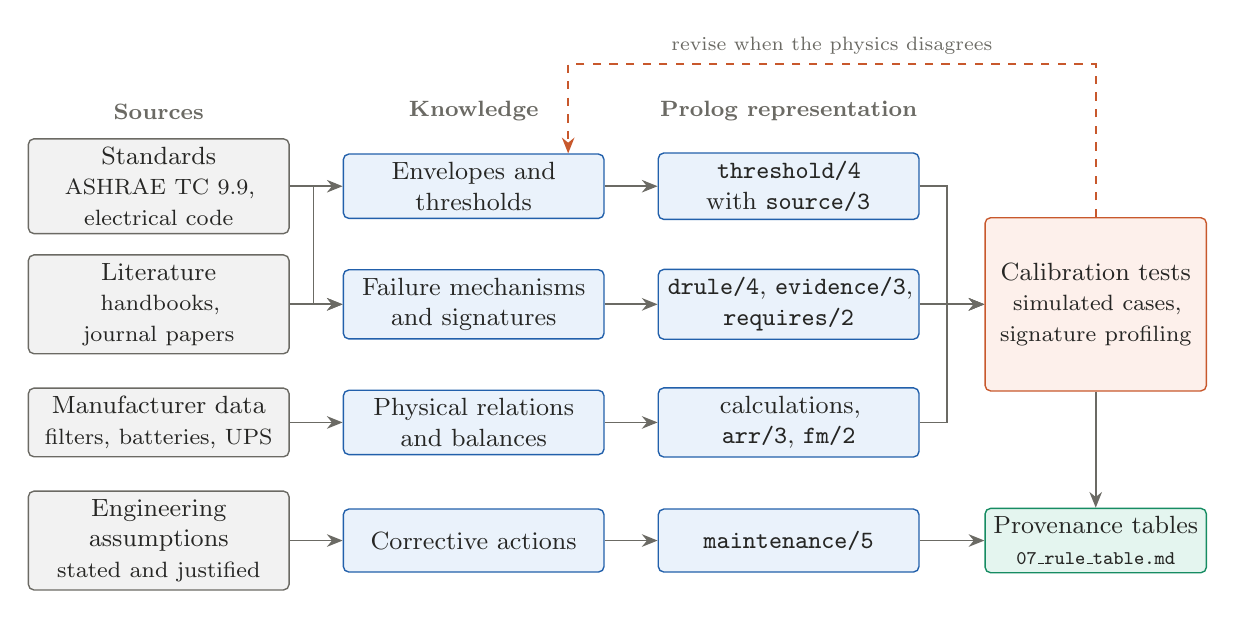
\begin{tikzpicture}[x=1cm, y=1cm]
  \node[grouplabel] at (1.6,0.95) {Sources};
  \node[data=3.1cm] (s1) at (1.6,0) {Standards\\ \footnotesize ASHRAE TC 9.9, electrical code};
  \node[data=3.1cm] (s2) at (1.6,-1.5) {Literature\\ \footnotesize handbooks, journal papers};
  \node[data=3.1cm] (s3) at (1.6,-3.0) {Manufacturer data\\ \footnotesize filters, batteries, UPS};
  \node[data=3.1cm] (s4) at (1.6,-4.5) {Engineering assumptions\\ \footnotesize stated and justified};

  \node[grouplabel] at (5.6,0.95) {Knowledge};
  \node[kb=3.1cm] (k1) at (5.6,0) {Envelopes and thresholds};
  \node[kb=3.1cm] (k2) at (5.6,-1.5) {Failure mechanisms and signatures};
  \node[kb=3.1cm] (k3) at (5.6,-3.0) {Physical relations and balances};
  \node[kb=3.1cm] (k4) at (5.6,-4.5) {Corrective actions};

  \node[grouplabel] at (9.6,0.95) {Prolog representation};
  \node[kb=3.1cm] (r1) at (9.6,0) {\texttt{threshold/4}\\ with \texttt{source/3}};
  \node[kb=3.1cm] (r2) at (9.6,-1.5) {\texttt{drule/4}, \texttt{evidence/3}, \texttt{requires/2}};
  \node[kb=3.1cm] (r3) at (9.6,-3.0) {calculations, \texttt{arr/3}, \texttt{fm/2}};
  \node[kb=3.1cm] (r4) at (9.6,-4.5) {\texttt{maintenance/5}};

  \node[reason=2.6cm, minimum height=2.2cm] (test) at (13.5,-1.5) {Calibration tests\\ \footnotesize simulated cases, signature profiling};
  \node[out=2.6cm] (table) at (13.5,-4.5) {Provenance tables\\ \scriptsize \texttt{07\_rule\_table.md}};

  \foreach \i in {1,2,3,4} { \draw[flow] (s\i) -- (k\i); \draw[flow] (k\i) -- (r\i); }
  \draw[flow] (s1.east) -- ++(0.3,0) |- (k2.west);
  \draw[flow] (r1.east) -- ++(0.35,0) |- (test.west);
  \draw[flow] (r2.east) -- (test.west |- r2.east);
  \draw[flow] (r3.east) -- ++(0.35,0) |- (test.west);
  \draw[flow] (r4) -- (table);
  \draw[flow] (test) -- (table);
  \draw[feedback] (test.north) -- (13.5,1.55) -- node[tag, above] {revise when the physics disagrees} (6.8,1.55) -- (k1.north -| 6.8,0);
\end{tikzpicture}

  \caption{Knowledge-acquisition workflow, from sources to Prolog representation, with feedback from calibration tests.}
  \label{fig:acquisition}
\end{figure}

\begin{table}[htbp]
  \centering
  \small
  \caption{Representative knowledge-acquisition entries.}
  \label{tab:acquisition}
  \begin{tabular}{L{4.0cm}L{3.4cm}L{6.6cm}}
    \toprule
    Knowledge & Source & Converted into \\
    \midrule
    Recommended inlet envelope 18 to 27\,\textdegree C & \textcite{ashrae2021} & Threshold facts; rule r01 \\
    Fan power scales with speed cubed & \textcite{ashraehvac2020} & Equation E23; rules r07, r08, r48, r49 \\
    Continuous load at most 80\% of rating & \textcite{nfpa702023} & Threshold fact; rule r17 \\
    Rising resistance indicates capacity fade & \textcite{ieee1188} & Equation E49; rule r18 \\
    Blanking panels prevent recirculation & Industry best practice (to verify) & Maintenance plan for $F_4$ \\
    Server power linear in utilisation & \textcite{fan2007} & Equation E1 \\
    Minimal diagnoses are minimal hitting sets & \textcite{reiter1987} & Consistency-based module \\
    Parsimonious covering & \textcite{peng1990} & Abductive module \\
    Fault models exonerate components & \textcite{struss1989} & \texttt{fm/2} facts \\
    \bottomrule
  \end{tabular}
\end{table}

\paragraph{Engineering assumptions.} Where no source gave a value for this particular row, the value was set by engineering reasoning and recorded as a source of type \texttt{assumption}. Examples are the 3\,K inlet stratification limit, chosen above the 1 to 2\,K seen in sealed racks, and the 0.85 fan power ratio, chosen well outside the $\pm$5\% scatter of a healthy fan. Of the 47 rules, 36 rest at least partly on such an assumption. Chapter~\ref{ch:dataset_and_evaluation} quantifies how sensitive the results are to each one, and shows that the large effects occur only when a threshold moves inside the scatter of normal operation.

\paragraph{Validation against a physics simulator.} Because no measured fault data were available, the knowledge was tested against cases generated by a steady-state simulator of the row, built from the equations of Section~\ref{sec:maths} (Chapter~\ref{ch:dataset_and_evaluation}). This exposed three errors that hand-made test cases had not revealed:
\begin{enumerate}
  \item The first rule for $F_2$ expected the chilled-water temperature rise to fall to zero. Physically, low flow makes it rise. The rule was rewritten to compare measured flow with the valve prediction (Equation E34a).
  \item A single-feed rack design ran at 81\% of its breaker rating in normal operation at high load, which would have made every overload rule fire falsely. The design was changed to dual feeds, as in real data centres.
  \item A rule that compared inlet and outlet stratification directly failed, because server fans speed up when their inlet air is hot. The final rules compare outlet stratification on its own with a fixed threshold (Equation E11a).
\end{enumerate}
In each case the knowledge was revised to agree with the physics, which is the feedback loop shown in Figure~\ref{fig:acquisition}. Thresholds were checked only against a calibration dataset. A separate held-out dataset was never used to adjust anything, so that the reported performance is not inflated by tuning.

\chapter{Design and Development of the Prolog Expert System}
\label{ch:design_and_development}

This chapter describes how the knowledge of Chapter~\ref{ch:theory_and_kr} was turned into a working expert system. It covers the architecture (Section~\ref{sec:architecture}), the design of the knowledge base (Section~\ref{sec:kb-design}), the predicates and rules (Section~\ref{sec:predicates}), the three inference mechanisms and their combination (Sections~\ref{sec:inference} to~\ref{sec:cbd}), the explanation facility (Section~\ref{sec:explanation}) and the corrective-maintenance planner (Section~\ref{sec:planner}). All diagnostic reasoning is implemented in SWI-Prolog. Python is used only to generate synthetic test data and to format results.

\lstset{language=Prolog, basicstyle=\ttfamily\footnotesize, columns=fullflexible, keepspaces=true,
        breaklines=true, frame=single, rulecolor=\color{black!35}, xleftmargin=2pt, xrightmargin=2pt,
        commentstyle=\color{black!60}\itshape, keywordstyle={}, showstringspaces=false}

% ---------------------------------------------------------------------------
\section{System Architecture}
\label{sec:architecture}

Figure~\ref{fig:architecture} shows the architecture. It follows the ten components that the project framework asks for:

\begin{enumerate}
  \item a user and input interface: test cases loaded as Prolog facts, and queries such as \texttt{why/1};
  \item observation and preprocessing predicates: noise estimation and graded symptoms;
  \item engineering-calculation predicates for the equations of Section~\ref{sec:maths};
  \item the knowledge base;
  \item a deductive inference engine;
  \item an abductive diagnosis module;
  \item a consistency-based diagnosis module;
  \item an explanation facility;
  \item a corrective-maintenance planner;
  \item an evaluation and reporting module.
\end{enumerate}

\begin{figure}[htbp]
  \centering
  % Figure 2: expert-system architecture.
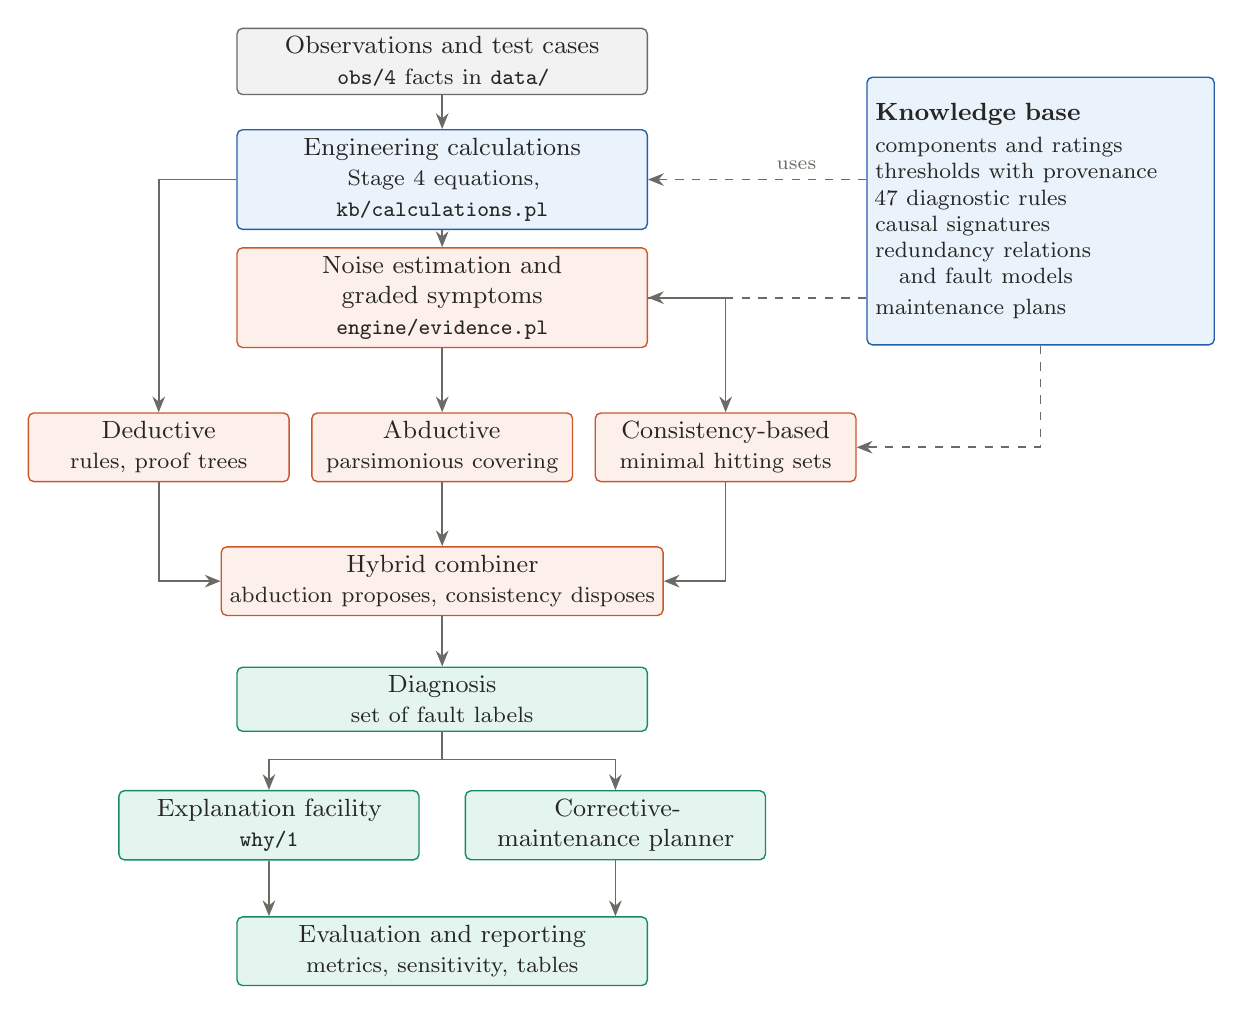
\begin{tikzpicture}[x=1cm, y=1cm]
  \node[data=5cm] (obs) at (4.5,0) {Observations and test cases\\ \footnotesize\texttt{obs/4} facts in \texttt{data/}};
  \node[kb=5cm] (calc) at (4.5,-1.5) {Engineering calculations\\ \footnotesize Stage 4 equations, \texttt{kb/calculations.pl}};
  \node[reason=5cm] (evid) at (4.5,-3.0) {Noise estimation and graded symptoms\\ \footnotesize \texttt{engine/evidence.pl}};

  \node[kb=4.2cm, minimum height=3.4cm, align=left] (kb) at (12.1,-1.9)
    {\textbf{Knowledge base}\\[2pt]
     \footnotesize components and ratings\\
     \footnotesize thresholds with provenance\\
     \footnotesize 47 diagnostic rules\\
     \footnotesize causal signatures\\
     \footnotesize redundancy relations\\
     \footnotesize \quad and fault models\\
     \footnotesize maintenance plans};

  \node[reason=3.1cm] (ded) at (0.9,-4.9) {Deductive\\ \footnotesize rules, proof trees};
  \node[reason=3.1cm] (abd) at (4.5,-4.9) {Abductive\\ \footnotesize parsimonious covering};
  \node[reason=3.1cm] (cbd) at (8.1,-4.9) {Consistency-based\\ \footnotesize minimal hitting sets};

  \node[reason=5.4cm] (hyb) at (4.5,-6.6) {Hybrid combiner\\ \footnotesize abduction proposes, consistency disposes};
  \node[out=5cm] (diag) at (4.5,-8.1) {Diagnosis\\ \footnotesize set of fault labels};
  \node[out=3.6cm] (expl) at (2.3,-9.7) {Explanation facility\\ \footnotesize \texttt{why/1}};
  \node[out=3.6cm] (maint) at (6.7,-9.7) {Corrective-maintenance planner};
  \node[out=5cm] (eval) at (4.5,-11.3) {Evaluation and reporting\\ \footnotesize metrics, sensitivity, tables};

  \draw[flow] (obs) -- (calc);
  \draw[flow] (calc) -- (evid);
  \draw[flow] (calc.west) -| (ded.north);
  \draw[flow] (evid) -- (abd);
  \draw[flow] (evid.east) -| (cbd.north);
  \draw[flow] (ded.south) |- (hyb.west);
  \draw[flow] (abd) -- (hyb);
  \draw[flow] (cbd.south) |- (hyb.east);
  \draw[flow] (hyb) -- (diag);
  \draw[flow] (diag.south) -- ++(0,-0.35) -| (expl.north);
  \draw[flow] (diag.south) -- ++(0,-0.35) -| (maint.north);
  \draw[flow] (expl.south) -- (expl.south |- eval.north);
  \draw[flow] (maint.south) -- (maint.south |- eval.north);

  \draw[uses] (kb.west |- calc.east) -- (calc.east);
  \draw[uses] (kb.west |- evid.east) -- (evid.east);
  \draw[uses] (kb.south) |- (cbd.east);
  \node[tag, anchor=south] at (9.0,-1.5) {uses};
\end{tikzpicture}

  \caption{Architecture of the Prolog expert system.}
  \label{fig:architecture}
\end{figure}

The knowledge base is kept separate from the engines that use it, which is the defining property of an expert system \parencite{jackson1998}. Table~\ref{tab:modules} lists the source files. The knowledge base and engines together are about 1{,}900 lines of Prolog, and the test and reporting code about 460 more. A single entry file, \texttt{main.pl}, loads everything.

\begin{table}[htbp]
  \centering
  \small
  \caption{Source modules.}
  \label{tab:modules}
  \begin{tabular}{L{4.8cm}L{9.2cm}}
    \toprule
    File & Role \\
    \midrule
    \texttt{kb/components.pl} & Components, topology, ratings and the variable dictionary \\
    \texttt{kb/thresholds.pl}, \texttt{kb/sources.pl} & Reference values and their provenance \\
    \texttt{kb/calculations.pl} & Engineering equations as predicates \\
    \texttt{kb/rules.pl} & Diagnostic rules stored as \texttt{drule/4} facts \\
    \texttt{kb/symptoms.pl} & Graded symptom definitions with noise models \\
    \texttt{kb/causal.pl} & Causal signatures for abduction \\
    \texttt{kb/arr.pl} & Redundancy relations and fault models \\
    \texttt{kb/maintenance.pl} & Corrective-maintenance plans and plan interactions \\
    \texttt{engine/prover.pl} & Proof-recording meta-interpreter \\
    \texttt{engine/deductive.pl} & Deductive diagnosis and closed-world conclusions \\
    \texttt{engine/evidence.pl} & Noise estimation and evidence grading \\
    \texttt{engine/abductive.pl} & Parsimonious covering \\
    \texttt{engine/consistency.pl} & Conflicts, minimal hitting sets and fault models \\
    \texttt{engine/hybrid.pl} & The four reasoning configurations \\
    \texttt{engine/explain.pl} & The explanation facility \\
    \texttt{tests/*.pl} & Test runner, metrics, sensitivity and table export \\
    \bottomrule
  \end{tabular}
\end{table}

% ---------------------------------------------------------------------------
\section{Knowledge-Base Design}
\label{sec:kb-design}

The knowledge base follows the seven layers of Table~\ref{tab:kr-layers}. Its contents are summarised in Table~\ref{tab:kb-size}.

\begin{table}[htbp]
  \centering
  \small
  \caption{Contents of the knowledge base.}
  \label{tab:kb-size}
  \begin{tabular}{L{7.0cm}L{2.0cm}L{5.0cm}}
    \toprule
    Element & Count & Representation \\
    \midrule
    Diagnostic rules deriving conditions & 29 & \texttt{drule/4} \\
    Diagnostic rules deriving faults & 18 & \texttt{drule/4} \\
    Closed-world conclusions & 2 & \texttt{engine/deductive.pl} \\
    Thresholds & 24 & \texttt{threshold/4} \\
    Sources: standard, literature, method, assumption & 3, 1, 3, 17 & \texttt{source/3} \\
    Engineering-calculation predicates & 20 & \texttt{calc\_pred/1} \\
    Graded, yes/no and composite symptoms & 20, 2, 2 & \texttt{sdef/7} and others \\
    Causal evidence links & 31 & \texttt{evidence/3} \\
    Required symptoms, masking links, extra explanations & 12, 2, 4 & \texttt{requires/2} and others \\
    Analytical redundancy relations & 20 & \texttt{arr/3} \\
    Fault models & 14 & \texttt{fm/2} \\
    Maintenance plans & 12 & \texttt{maintenance/5} \\
    Plan interactions & 4 & \texttt{plan\_interaction/3} \\
    \bottomrule
  \end{tabular}
\end{table}

\subsection{Facts}

Structural knowledge is stated as ground facts, for example \texttt{component(crah\_1, crah)}, \texttt{serves(crah\_1, rack\_a04)} and \texttt{rated(crah\_1, fan\_power\_rated, 5.5, kw)}. Observations are facts \texttt{obs(Case, Variable, Entity, Value)}, so every case is a self-contained set of facts and the same knowledge base diagnoses all cases.

\subsection{Thresholds and provenance}

Each threshold is a fact with its value, unit and source, and each source has a type:
\begin{lstlisting}
threshold(t_inlet_rec_max, 27.0, degC, ashrae_tc99_2021).
threshold(strat_out_max,    3.5, kelvin, a7_outlet_strat).
source(a7_outlet_strat, assumption,
       'Engineering assumption: a top-to-bottom outlet difference above 3.5 K
        confirms recirculation. Normal racks stay below 3 K.').
\end{lstlisting}
Rules and symptoms refer to thresholds by name through \texttt{threshold/2}, never by value. A threshold can therefore be changed in one place, and the sensitivity analysis of Chapter~\ref{ch:dataset_and_evaluation} can perturb it without touching any rule. The complete threshold and provenance tables are generated from these facts (Tables~\ref{tab:thresholds} and~\ref{tab:provenance}).

\subsection{Engineering calculations}

Each equation of Section~\ref{sec:maths} that the reasoning needs is a Horn clause with arithmetic, commented with its equation tag. For example, the fan affinity law and the fan power ratio, Equations E23 and E24, are:
\begin{lstlisting}
%   Eq. 23  P_f,exp = P_f,rated * (N / N_rated)^3      fan affinity law
expected_fan_power(C, U, P) :-
    obs(C, fan_speed, U, N),
    rated(U, fan_power_rated, Pr, _),
    rated(U, fan_speed_rated, Nr, _),
    P is Pr * (N / Nr) ** 3.

%   Eq. 24  rho_f = P_f,measured / P_f,exp
fan_power_ratio(C, U, Ratio) :-
    obs(C, fan_power, U, Pm),
    expected_fan_power(C, U, Pe),
    Pe > 0,
    Ratio is Pm / Pe.
\end{lstlisting}
A calculation fails when one of its inputs is missing, and a rule that uses it then cannot fire. This is how incomplete evidence is handled in the deductive mode.

% ---------------------------------------------------------------------------
\section{Predicates and Rules}
\label{sec:predicates}

Table~\ref{tab:predicates} lists the main predicates. The diagnostic rules are listed in full in Table~\ref{tab:rules}, which is generated from \texttt{kb/rules.pl}. Each rule is a Horn clause stored as data:
\begin{lstlisting}
%   R24  F4 from exhaust evidence alone, when the top inlet sensor is
%        suspect because it reads low.
drule(r24, fault(C, hot_air_recirculation(R)),
      [ cond(C, outlet_stratified(R)), cond(C, inlet_not_stratified(R)),
        serves(U, R), cond(C, supply_air_normal(U)) ],
      eu_coc_dc).
\end{lstlisting}
It reads: rack $R$ has hot-air recirculation if its exhaust is stratified, its inlet reading is not, and its cooling unit supplies normal air. The rule exists because a low-reading top sensor can hide real recirculation (Table~\ref{tab:interactions}). The exhaust then carries the evidence that the inlet sensor does not.

\begin{table}[htbp]
  \centering
  \small
  \caption{Main predicates.}
  \label{tab:predicates}
  \begin{tabular}{L{4.6cm}L{9.4cm}}
    \toprule
    Predicate & Purpose \\
    \midrule
    \texttt{obs(C, V, E, X)} & Observation: variable $V$ of entity $E$ in case $C$ has value $X$ \\
    \texttt{threshold(N, X)} & Value of threshold $N$, after any sensitivity perturbation \\
    \texttt{drule(Id, H, B, S)} & Diagnostic rule $H \leftarrow B$ with identifier and source \\
    \texttt{prove(G, P)} & Proves goal $G$ and returns its proof tree $P$ \\
    \texttt{diagnose(C, Ds)} & Deductive diagnosis with proofs \\
    \texttt{case\_symptoms(C, Ss)} & Graded symptoms with evidence and status \\
    \texttt{abduce(C, R)} & Abductive candidates, minimal explanations and verdicts \\
    \texttt{conflicts(Ss, Ks)} & Conflict sets from violated redundancy relations \\
    \texttt{cbd\_diagnoses(Ss, Ds)} & Minimal consistent diagnoses \\
    \texttt{diagnose\_mode(M, C, Ls)} & Diagnosis in configuration $M$ \\
    \texttt{why(C)} & Full explanation of the complete system's diagnosis \\
    \texttt{maintenance(K, Pr, As, R, S)} & Plan for fault class $K$: priority, actions, rationale, source \\
    \bottomrule
  \end{tabular}
\end{table}

% Generated by tests/export_latex.pl from the knowledge base. Do not edit by hand.
\begin{footnotesize}
\begin{longtable}{L{0.9cm}L{4.0cm}L{7.0cm}L{1.9cm}}
  \caption{Diagnostic rules, generated from \texttt{kb/rules.pl}. In each rule \texttt{A} is the case being diagnosed and \texttt{\textbackslash+} is negation as failure.}\label{tab:rules}\\
  \toprule
  Rule & Concludes & If all of these hold & Source type \\
  \midrule
  \endfirsthead
  \toprule
  Rule & Concludes & If all of these hold & Source type \\
  \midrule
  \endhead
  \texttt{r01} & condition \texttt{rack\_\allowbreak{}inlet\_\allowbreak{}hot(B)} & \texttt{component(B,\allowbreak{} rack), \allowbreak inlet\_\allowbreak{}max(A,\allowbreak{} B,\allowbreak{} C), \allowbreak threshold(t\_\allowbreak{}inlet\_\allowbreak{}rec\_\allowbreak{}max,\allowbreak{} D), \allowbreak C>D} & standard \\
  \texttt{r02} & condition \texttt{row\_\allowbreak{}inlet\_\allowbreak{}hot} & \texttt{hot\_\allowbreak{}rack\_\allowbreak{}fraction(A,\allowbreak{} B), \allowbreak threshold(row\_\allowbreak{}hot\_\allowbreak{}fraction,\allowbreak{} C), \allowbreak B>=C} & assumption \\
  \texttt{r03} & condition \texttt{localised\_\allowbreak{}inlet\_\allowbreak{}hot(B)} & \texttt{cond(A,\allowbreak{} rack\_\allowbreak{}inlet\_\allowbreak{}hot(B)), \allowbreak hot\_\allowbreak{}rack\_\allowbreak{}fraction(A,\allowbreak{} C), \allowbreak threshold(row\_\allowbreak{}hot\_\allowbreak{}fraction,\allowbreak{} D), \allowbreak C<D} & assumption \\
  \texttt{r04} & condition \texttt{inlet\_\allowbreak{}stratified(B)} & \texttt{inlet\_\allowbreak{}stratification(A,\allowbreak{} B,\allowbreak{} C), \allowbreak threshold(strat\_\allowbreak{}max,\allowbreak{} D), \allowbreak C>D} & assumption \\
  \texttt{r05} & condition \texttt{supply\_\allowbreak{}air\_\allowbreak{}hot(B)} & \texttt{component(B,\allowbreak{} crah), \allowbreak obs(A,\allowbreak{} t\_\allowbreak{}supply\_\allowbreak{}air,\allowbreak{} B,\allowbreak{} C), \allowbreak threshold(t\_\allowbreak{}supply\_\allowbreak{}setpoint,\allowbreak{} D), \allowbreak threshold(t\_\allowbreak{}supply\_\allowbreak{}band,\allowbreak{} E), \allowbreak C>D+E} & assumption \\
  \texttt{r06} & condition \texttt{supply\_\allowbreak{}air\_\allowbreak{}normal(B)} & \texttt{component(B,\allowbreak{} crah), \allowbreak obs(A,\allowbreak{} t\_\allowbreak{}supply\_\allowbreak{}air,\allowbreak{} B,\allowbreak{} C), \allowbreak threshold(t\_\allowbreak{}supply\_\allowbreak{}setpoint,\allowbreak{} D), \allowbreak threshold(t\_\allowbreak{}supply\_\allowbreak{}band,\allowbreak{} E), \allowbreak C=<D+E} & assumption \\
  \texttt{r07} & condition \texttt{fan\_\allowbreak{}power\_\allowbreak{}low(B)} & \texttt{component(B,\allowbreak{} crah), \allowbreak fan\_\allowbreak{}power\_\allowbreak{}ratio(A,\allowbreak{} B,\allowbreak{} C), \allowbreak threshold(fan\_\allowbreak{}ratio\_\allowbreak{}min,\allowbreak{} D), \allowbreak C<D} & assumption \\
  \texttt{r08} & condition \texttt{fan\_\allowbreak{}power\_\allowbreak{}normal(B)} & \texttt{component(B,\allowbreak{} crah), \allowbreak fan\_\allowbreak{}power\_\allowbreak{}ratio(A,\allowbreak{} B,\allowbreak{} C), \allowbreak threshold(fan\_\allowbreak{}ratio\_\allowbreak{}min,\allowbreak{} D), \allowbreak C>=D} & literature \\
  \texttt{r09} & condition \texttt{valve\_\allowbreak{}open(B)} & \texttt{obs(A,\allowbreak{} valve\_\allowbreak{}position,\allowbreak{} B,\allowbreak{} C), \allowbreak threshold(valve\_\allowbreak{}open\_\allowbreak{}min,\allowbreak{} D), \allowbreak C>=D} & assumption \\
  \texttt{r10} & condition \texttt{chw\_\allowbreak{}flow\_\allowbreak{}low(B)} & \texttt{chw\_\allowbreak{}flow\_\allowbreak{}ratio(A,\allowbreak{} B,\allowbreak{} C), \allowbreak threshold(chw\_\allowbreak{}flow\_\allowbreak{}ratio\_\allowbreak{}min,\allowbreak{} D), \allowbreak C<D} & assumption \\
  \texttt{r20} & fault \texttt{crah\_\allowbreak{}fan\_\allowbreak{}failure(B)} & \texttt{cond(A,\allowbreak{} row\_\allowbreak{}inlet\_\allowbreak{}hot), \allowbreak cond(A,\allowbreak{} fan\_\allowbreak{}power\_\allowbreak{}low(B))} & literature \\
  \texttt{r21} & fault \texttt{chw\_\allowbreak{}supply\_\allowbreak{}loss(B)} & \texttt{cond(A,\allowbreak{} supply\_\allowbreak{}air\_\allowbreak{}hot(B)), \allowbreak cond(A,\allowbreak{} valve\_\allowbreak{}open(B)), \allowbreak cond(A,\allowbreak{} chw\_\allowbreak{}flow\_\allowbreak{}low(B)), \allowbreak cond(A,\allowbreak{} fan\_\allowbreak{}power\_\allowbreak{}normal(B))} & assumption \\
  \texttt{r11} & condition \texttt{outlet\_\allowbreak{}stratified(B)} & \texttt{outlet\_\allowbreak{}stratification(A,\allowbreak{} B,\allowbreak{} C), \allowbreak threshold(strat\_\allowbreak{}out\_\allowbreak{}max,\allowbreak{} D), \allowbreak C>D} & assumption \\
  \texttt{r12} & condition \texttt{outlet\_\allowbreak{}not\_\allowbreak{}stratified(B)} & \texttt{outlet\_\allowbreak{}stratification(A,\allowbreak{} B,\allowbreak{} C), \allowbreak threshold(strat\_\allowbreak{}out\_\allowbreak{}max,\allowbreak{} D), \allowbreak C=<D} & assumption \\
  \texttt{r13} & condition \texttt{inlet\_\allowbreak{}not\_\allowbreak{}stratified(B)} & \texttt{inlet\_\allowbreak{}stratification(A,\allowbreak{} B,\allowbreak{} C), \allowbreak threshold(strat\_\allowbreak{}max,\allowbreak{} D), \allowbreak C=<D} & assumption \\
  \texttt{r14} & condition \texttt{filter\_\allowbreak{}loaded(B)} & \texttt{component(B,\allowbreak{} crah), \allowbreak filter\_\allowbreak{}loading(A,\allowbreak{} B,\allowbreak{} C), \allowbreak threshold(filter\_\allowbreak{}loading\_\allowbreak{}max,\allowbreak{} D), \allowbreak C>D} & assumption \\
  \texttt{r15} & condition \texttt{server\_\allowbreak{}fan\_\allowbreak{}stopped(B)} & \texttt{obs(A,\allowbreak{} server\_\allowbreak{}fan\_\allowbreak{}rpm,\allowbreak{} B,\allowbreak{} C), \allowbreak threshold(server\_\allowbreak{}fan\_\allowbreak{}min,\allowbreak{} D), \allowbreak C<D} & assumption \\
  \texttt{r16} & condition \texttt{cpu\_\allowbreak{}hot(B)} & \texttt{obs(A,\allowbreak{} t\_\allowbreak{}cpu,\allowbreak{} B,\allowbreak{} C), \allowbreak threshold(cpu\_\allowbreak{}hot\_\allowbreak{}min,\allowbreak{} D), \allowbreak C>=D} & assumption \\
  \texttt{r17} & condition \texttt{branch\_\allowbreak{}overloaded(B)} & \texttt{branch\_\allowbreak{}loading(A,\allowbreak{} B,\allowbreak{} C), \allowbreak threshold(branch\_\allowbreak{}loading\_\allowbreak{}max,\allowbreak{} D), \allowbreak C>D} & standard \\
  \texttt{r18} & condition \texttt{cell\_\allowbreak{}resistance\_\allowbreak{}high(B)} & \texttt{component(B,\allowbreak{} battery), \allowbreak cell\_\allowbreak{}resistance\_\allowbreak{}ratio(A,\allowbreak{} B,\allowbreak{} C), \allowbreak threshold(cell\_\allowbreak{}r\_\allowbreak{}ratio\_\allowbreak{}max,\allowbreak{} D), \allowbreak C>D} & assumption \\
  \texttt{r19} & condition \texttt{ups\_\allowbreak{}efficiency\_\allowbreak{}bypass\_\allowbreak{}like(B)} & \texttt{component(B,\allowbreak{} ups), \allowbreak ups\_\allowbreak{}efficiency(A,\allowbreak{} B,\allowbreak{} C), \allowbreak threshold(ups\_\allowbreak{}eff\_\allowbreak{}bypass\_\allowbreak{}min,\allowbreak{} D), \allowbreak C>=D} & assumption \\
  \texttt{r40} & condition \texttt{mid\_\allowbreak{}inlet\_\allowbreak{}deviates(B)} & \texttt{component(B,\allowbreak{} rack), \allowbreak mid\_\allowbreak{}inlet\_\allowbreak{}deviation(A,\allowbreak{} B,\allowbreak{} C), \allowbreak threshold(neighbour\_\allowbreak{}dev\_\allowbreak{}max,\allowbreak{} D), \allowbreak abs(C)>D, \allowbreak \textbackslash{}+cond(A,\allowbreak{} inlet\_\allowbreak{}rise\_\allowbreak{}corroborated(B))} & assumption \\
  \texttt{r45} & condition \texttt{inlet\_\allowbreak{}rise\_\allowbreak{}corroborated(B)} & \texttt{mid\_\allowbreak{}inlet\_\allowbreak{}deviation(A,\allowbreak{} B,\allowbreak{} C), \allowbreak top\_\allowbreak{}inlet\_\allowbreak{}deviation(A,\allowbreak{} B,\allowbreak{} D), \allowbreak C*D>0, \allowbreak threshold(neighbour\_\allowbreak{}dev\_\allowbreak{}max,\allowbreak{} E), \allowbreak abs(D)>E} & assumption \\
  \texttt{r46} & condition \texttt{top\_\allowbreak{}inlet\_\allowbreak{}sensor\_\allowbreak{}suspect(B)} & \texttt{component(B,\allowbreak{} rack), \allowbreak inlet\_\allowbreak{}stratification(A,\allowbreak{} B,\allowbreak{} C), \allowbreak threshold(neighbour\_\allowbreak{}dev\_\allowbreak{}max,\allowbreak{} D), \allowbreak C< -D, \allowbreak \textbackslash{}+cond(A,\allowbreak{} mid\_\allowbreak{}inlet\_\allowbreak{}deviates(B))} & method \\
  \texttt{r41} & condition \texttt{top\_\allowbreak{}inlet\_\allowbreak{}sensor\_\allowbreak{}suspect(B)} & \texttt{cond(A,\allowbreak{} inlet\_\allowbreak{}stratified(B)), \allowbreak cond(A,\allowbreak{} outlet\_\allowbreak{}not\_\allowbreak{}stratified(B)), \allowbreak \textbackslash{}+cond(A,\allowbreak{} mid\_\allowbreak{}inlet\_\allowbreak{}deviates(B))} & assumption \\
  \texttt{r42} & condition \texttt{top\_\allowbreak{}inlet\_\allowbreak{}sensor\_\allowbreak{}suspect(B)} & \texttt{cond(A,\allowbreak{} outlet\_\allowbreak{}stratified(B)), \allowbreak cond(A,\allowbreak{} inlet\_\allowbreak{}not\_\allowbreak{}stratified(B)), \allowbreak \textbackslash{}+cond(A,\allowbreak{} mid\_\allowbreak{}inlet\_\allowbreak{}deviates(B))} & assumption \\
  \texttt{r43} & condition \texttt{supply\_\allowbreak{}sensor\_\allowbreak{}inconsistent(B)} & \texttt{component(B,\allowbreak{} crah), \allowbreak cond(A,\allowbreak{} fan\_\allowbreak{}power\_\allowbreak{}nominal(B)), \allowbreak supply\_\allowbreak{}air\_\allowbreak{}deviation(A,\allowbreak{} B,\allowbreak{} C), \allowbreak threshold(neighbour\_\allowbreak{}dev\_\allowbreak{}max,\allowbreak{} D), \allowbreak abs(C)>D, \allowbreak coil\_\allowbreak{}balance\_\allowbreak{}residual(A,\allowbreak{} B,\allowbreak{} E), \allowbreak threshold(balance\_\allowbreak{}resid\_\allowbreak{}max,\allowbreak{} F), \allowbreak abs(E)>F, \allowbreak coil\_\allowbreak{}balance\_\allowbreak{}residual\_\allowbreak{}corrected(A,\allowbreak{} B,\allowbreak{} G), \allowbreak abs(G)=<F} & method \\
  \texttt{r48} & condition \texttt{fan\_\allowbreak{}power\_\allowbreak{}nominal(B)} & \texttt{component(B,\allowbreak{} crah), \allowbreak fan\_\allowbreak{}power\_\allowbreak{}ratio(A,\allowbreak{} B,\allowbreak{} C), \allowbreak threshold(fan\_\allowbreak{}ratio\_\allowbreak{}reduced,\allowbreak{} D), \allowbreak C>=D} & assumption \\
  \texttt{r49} & condition \texttt{fan\_\allowbreak{}power\_\allowbreak{}reduced(B)} & \texttt{component(B,\allowbreak{} crah), \allowbreak fan\_\allowbreak{}power\_\allowbreak{}ratio(A,\allowbreak{} B,\allowbreak{} C), \allowbreak threshold(fan\_\allowbreak{}ratio\_\allowbreak{}reduced,\allowbreak{} D), \allowbreak C<D} & assumption \\
  \texttt{r47} & condition \texttt{supply\_\allowbreak{}air\_\allowbreak{}cold(B)} & \texttt{component(B,\allowbreak{} crah), \allowbreak obs(A,\allowbreak{} t\_\allowbreak{}supply\_\allowbreak{}air,\allowbreak{} B,\allowbreak{} C), \allowbreak threshold(t\_\allowbreak{}supply\_\allowbreak{}setpoint,\allowbreak{} D), \allowbreak threshold(t\_\allowbreak{}supply\_\allowbreak{}band,\allowbreak{} E), \allowbreak C<D-E} & assumption \\
  \texttt{r44} & condition \texttt{telemetry\_\allowbreak{}stale(B)} & \texttt{obs(A,\allowbreak{} sample\_\allowbreak{}age,\allowbreak{} B,\allowbreak{} C), \allowbreak threshold(sample\_\allowbreak{}age\_\allowbreak{}max,\allowbreak{} D), \allowbreak C>D} & assumption \\
  \texttt{r36} & fault \texttt{crah\_\allowbreak{}fan\_\allowbreak{}failure(B)} & \texttt{cond(A,\allowbreak{} row\_\allowbreak{}inlet\_\allowbreak{}hot), \allowbreak cond(A,\allowbreak{} supply\_\allowbreak{}air\_\allowbreak{}cold(B)), \allowbreak \textbackslash{}+cond(A,\allowbreak{} supply\_\allowbreak{}sensor\_\allowbreak{}inconsistent(B))} & assumption \\
  \texttt{r38} & fault \texttt{crah\_\allowbreak{}fan\_\allowbreak{}failure(B)} & \texttt{cond(A,\allowbreak{} fan\_\allowbreak{}power\_\allowbreak{}reduced(B)), \allowbreak cond(A,\allowbreak{} row\_\allowbreak{}inlet\_\allowbreak{}hot)} & assumption \\
  \texttt{r37} & fault \texttt{chw\_\allowbreak{}supply\_\allowbreak{}loss(B)} & \texttt{cond(A,\allowbreak{} supply\_\allowbreak{}air\_\allowbreak{}hot(B)), \allowbreak cond(A,\allowbreak{} valve\_\allowbreak{}open(B)), \allowbreak cond(A,\allowbreak{} fan\_\allowbreak{}power\_\allowbreak{}normal(B)), \allowbreak \textbackslash{}+obs(A,\allowbreak{} m\_\allowbreak{}chw,\allowbreak{} B,\allowbreak{} C), \allowbreak \textbackslash{}+cond(A,\allowbreak{} supply\_\allowbreak{}sensor\_\allowbreak{}inconsistent(B))} & assumption \\
  \texttt{r22} & fault \texttt{hot\_\allowbreak{}air\_\allowbreak{}recirculation(B)} & \texttt{cond(A,\allowbreak{} localised\_\allowbreak{}inlet\_\allowbreak{}hot(B)), \allowbreak serves(C,\allowbreak{} B), \allowbreak cond(A,\allowbreak{} supply\_\allowbreak{}air\_\allowbreak{}normal(C)), \allowbreak cond(A,\allowbreak{} inlet\_\allowbreak{}stratified(B)), \allowbreak \textbackslash{}+cond(A,\allowbreak{} top\_\allowbreak{}inlet\_\allowbreak{}sensor\_\allowbreak{}suspect(B))} & standard \\
  \texttt{r23} & fault \texttt{hot\_\allowbreak{}air\_\allowbreak{}recirculation(B)} & \texttt{cond(A,\allowbreak{} inlet\_\allowbreak{}stratified(B)), \allowbreak cond(A,\allowbreak{} outlet\_\allowbreak{}stratified(B)), \allowbreak serves(C,\allowbreak{} B), \allowbreak cond(A,\allowbreak{} supply\_\allowbreak{}air\_\allowbreak{}normal(C))} & standard \\
  \texttt{r24} & fault \texttt{hot\_\allowbreak{}air\_\allowbreak{}recirculation(B)} & \texttt{cond(A,\allowbreak{} outlet\_\allowbreak{}stratified(B)), \allowbreak cond(A,\allowbreak{} inlet\_\allowbreak{}not\_\allowbreak{}stratified(B)), \allowbreak serves(C,\allowbreak{} B), \allowbreak cond(A,\allowbreak{} supply\_\allowbreak{}air\_\allowbreak{}normal(C))} & standard \\
  \texttt{r25} & fault \texttt{filter\_\allowbreak{}clogging(B)} & \texttt{cond(A,\allowbreak{} filter\_\allowbreak{}loaded(B)), \allowbreak cond(A,\allowbreak{} fan\_\allowbreak{}power\_\allowbreak{}normal(B))} & assumption \\
  \texttt{r26} & fault \texttt{server\_\allowbreak{}fan\_\allowbreak{}failure(B)} & \texttt{cond(A,\allowbreak{} server\_\allowbreak{}fan\_\allowbreak{}stopped(B)), \allowbreak cond(A,\allowbreak{} cpu\_\allowbreak{}hot(B))} & assumption \\
  \texttt{r27} & fault \texttt{branch\_\allowbreak{}overload(B)} & \texttt{cond(A,\allowbreak{} branch\_\allowbreak{}overloaded(B))} & standard \\
  \texttt{r28} & fault \texttt{battery\_\allowbreak{}degradation(B)} & \texttt{cond(A,\allowbreak{} cell\_\allowbreak{}resistance\_\allowbreak{}high(B))} & assumption \\
  \texttt{r29} & fault \texttt{ups\_\allowbreak{}on\_\allowbreak{}bypass(B)} & \texttt{component(B,\allowbreak{} ups), \allowbreak obs(A,\allowbreak{} ups\_\allowbreak{}mode,\allowbreak{} B,\allowbreak{} bypass)} & assumption \\
  \texttt{r35} & fault \texttt{ups\_\allowbreak{}on\_\allowbreak{}bypass(B)} & \texttt{component(B,\allowbreak{} ups), \allowbreak \textbackslash{}+obs(A,\allowbreak{} ups\_\allowbreak{}mode,\allowbreak{} B,\allowbreak{} C), \allowbreak cond(A,\allowbreak{} ups\_\allowbreak{}efficiency\_\allowbreak{}bypass\_\allowbreak{}like(B))} & assumption \\
  \texttt{r50} & fault \texttt{sensor\_\allowbreak{}bias(t\_\allowbreak{}inlet\_\allowbreak{}mid,\allowbreak{} B)} & \texttt{cond(A,\allowbreak{} mid\_\allowbreak{}inlet\_\allowbreak{}deviates(B))} & assumption \\
  \texttt{r51} & fault \texttt{sensor\_\allowbreak{}bias(t\_\allowbreak{}inlet\_\allowbreak{}top,\allowbreak{} B)} & \texttt{cond(A,\allowbreak{} top\_\allowbreak{}inlet\_\allowbreak{}sensor\_\allowbreak{}suspect(B))} & assumption \\
  \texttt{r52} & fault \texttt{sensor\_\allowbreak{}bias(t\_\allowbreak{}supply\_\allowbreak{}air,\allowbreak{} B)} & \texttt{cond(A,\allowbreak{} supply\_\allowbreak{}sensor\_\allowbreak{}inconsistent(B))} & method \\
  \texttt{r53} & fault \texttt{telemetry\_\allowbreak{}dropout(B)} & \texttt{cond(A,\allowbreak{} telemetry\_\allowbreak{}stale(B))} & assumption \\
  \texttt{r30} & fault \texttt{normal} & no fault rule fires, and every rack inlet is within the recommended envelope & method \\
  \texttt{r31} & \texttt{unexplained\_\allowbreak{}abnormality} & no fault rule fires, but some rack inlet is outside the envelope & method \\
  \bottomrule
\end{longtable}
\end{footnotesize}


% ---------------------------------------------------------------------------
\section{Inference Mechanisms}
\label{sec:inference}

Figure~\ref{fig:diagnostic} shows how the three inference mechanisms work together on one case. The readings are first used to estimate measurement noise. Every symptom is then graded. Deductive rules, abduction and consistency checking run on the result, and the hybrid combiner chooses the final diagnosis.

\begin{figure}[htbp]
  \centering
  % Figure 5: diagnostic reasoning workflow of the complete system.
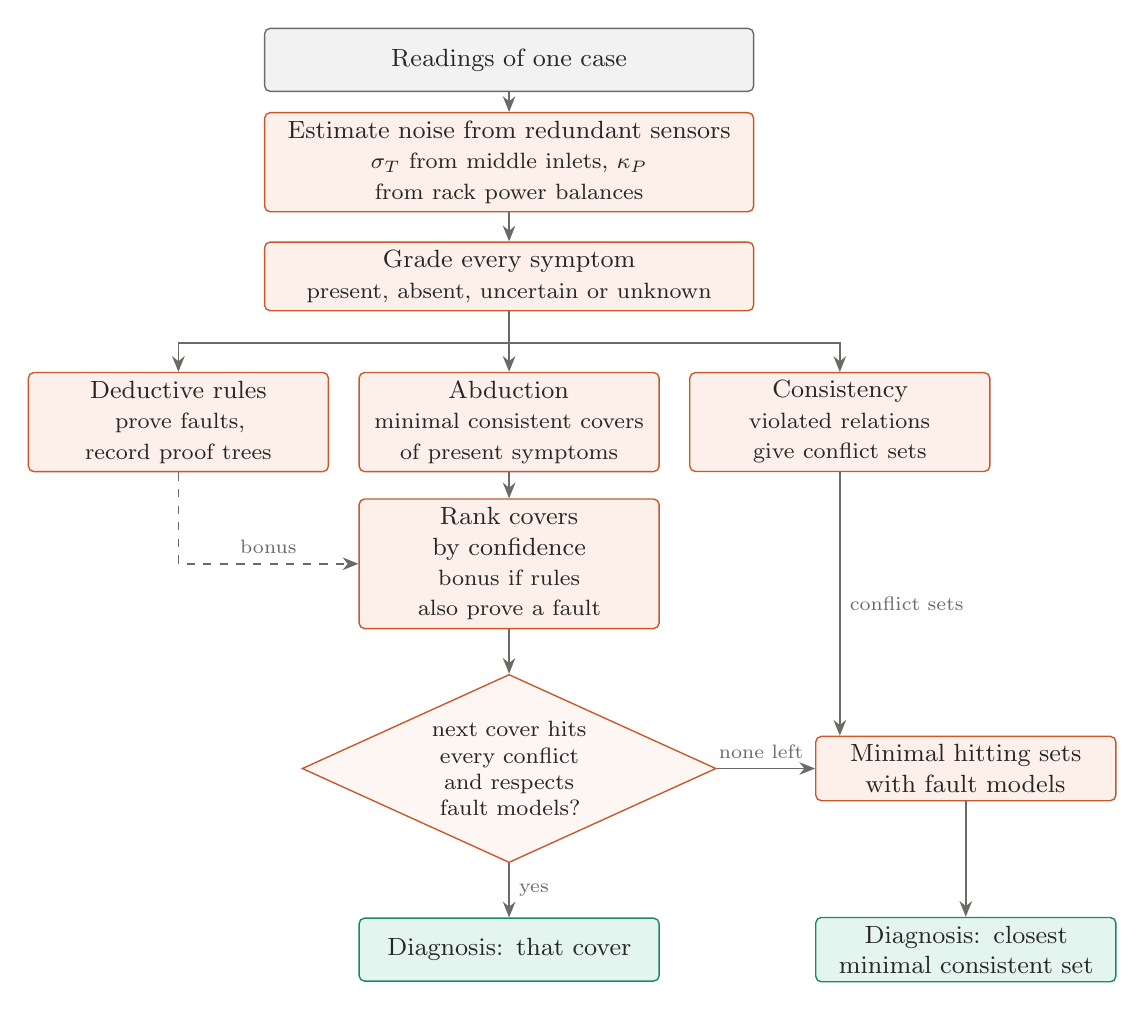
\begin{tikzpicture}[x=1cm, y=1cm]
  \node[data=6cm] (obs) at (4.5,0) {Readings of one case};
  \node[reason=6cm] (noise) at (4.5,-1.3) {Estimate noise from redundant sensors\\ \footnotesize $\sigma_T$ from middle inlets, $\kappa_P$ from rack power balances};
  \node[reason=6cm] (grade) at (4.5,-2.75) {Grade every symptom\\ \footnotesize present, absent, uncertain or unknown};

  \node[reason=3.6cm] (ded) at (0.3,-4.6) {Deductive rules\\ \footnotesize prove faults, record proof trees};
  \node[reason=3.6cm] (abd) at (4.5,-4.6) {Abduction\\ \footnotesize minimal consistent covers of present symptoms};
  \node[reason=3.6cm] (cbd) at (8.7,-4.6) {Consistency\\ \footnotesize violated relations give conflict sets};

  \node[reason=3.6cm] (rank) at (4.5,-6.4) {Rank covers by confidence\\ \footnotesize bonus if rules also prove a fault};
  \node[decision=2.4cm] (dec) at (4.5,-9.0) {next cover hits every conflict and respects fault models?};
  \node[reason=3.6cm] (mhs) at (10.3,-9.0) {Minimal hitting sets with fault models};
  \node[out=3.6cm] (yes) at (4.5,-11.3) {Diagnosis: that cover};
  \node[out=3.6cm] (no) at (10.3,-11.3) {Diagnosis: closest minimal consistent set};

  \draw[flow] (obs) -- (noise);
  \draw[flow] (noise) -- (grade);
  \draw[flow] (grade.south) -- ++(0,-0.4) -| (ded.north);
  \draw[flow] (grade) -- (abd);
  \draw[flow] (grade.south) -- ++(0,-0.4) -| (cbd.north);
  \draw[flow] (abd) -- (rank);
  \draw[uses] (ded.south) |- node[tag, pos=0.75, above] {bonus} (rank.west);
  \draw[flow] (rank) -- (dec);
  \draw[flow] (dec) -- node[tag, right] {yes} (yes);
  \draw[flow] (dec) -- node[tag, above, pos=0.45] {none left} (mhs);
  \draw[flow] (cbd.south) -- node[tag, right] {conflict sets} (cbd.south |- mhs.north);
  \draw[flow] (mhs) -- (no);
\end{tikzpicture}

  \caption{Diagnostic reasoning workflow of the complete system: abduction proposes, consistency disposes.}
  \label{fig:diagnostic}
\end{figure}

\subsection{Graded, noise-adaptive evidence}

For each symptom definition, \texttt{engine/evidence.pl} computes the feature value, compares it with its threshold and grades the evidence with Equation E55. The noise $\sigma_j$ of each feature is propagated from the datasheet accuracy of its sensors and scaled by the noise level estimated from the case. For temperature features this is the robust spread of the six middle inlets, and for electrical features the spread of the six rack power balances. A symptom is \emph{present} once its value is one standard deviation past the threshold, \emph{absent} once it is one standard deviation on the normal side, and \emph{uncertain} in between. If an input is missing the symptom is \emph{unknown}, which is never treated as absent. The graded symptoms of a case are computed once and cached, so that the abductive and consistency-based modules see exactly the same evidence.

\subsection{The four configurations}

The framework asks for four configurations to be compared, and \texttt{engine/hybrid.pl} provides them through \texttt{diagnose\_mode/3}:

\begin{itemize}
  \item \textbf{Deductive only:} the rules of Table~\ref{tab:rules}.
  \item \textbf{Deductive and abductive:} the best parsimonious explanation, with a bonus of 0.1 to the confidence of hypotheses that the rules also prove.
  \item \textbf{Deductive and consistency-based:} the deductive faults are kept if they form a consistent diagnosis, after dropping any fault whose component hits no conflict. Otherwise the minimal consistent diagnosis closest to them replaces them.
  \item \textbf{Complete system:} abduction proposes and consistency disposes. The best-ranked abductive explanation that is also a consistent diagnosis is accepted. If none is consistent, the minimal consistent diagnosis closest to the top explanation is used.
\end{itemize}
When several consistent diagnoses tie, the one with fewer sensor components wins, because assuming a physical fault is the safer maintenance choice.

% ---------------------------------------------------------------------------
\section{Deductive Reasoning}
\label{sec:deductive}

Deductive diagnosis implements Equation~\eqref{eq:deductive}. Because rules are stored as data, a small meta-interpreter is needed to prove them \parencite{bratko2012}. It returns a proof tree for every conclusion:
\begin{lstlisting}
derived(cond(_, _)).
derived(fault(_, _)).

prove(\+ G, naf(G)) :-                 % negation as failure
    !,
    \+ prove(G, _).
prove(G, by(Id, G, SubProofs)) :-      % a derived goal: try each rule
    derived(G),
    !,
    drule(Id, G, Body, _),
    prove_body(Body, SubProofs).
prove(G, leaf(G)) :-                   % a fact, calculation or comparison
    call(G).

prove_body([], []).
prove_body([G|Gs], [P|Ps]) :-
    prove(G, P),
    prove_body(Gs, Ps).
\end{lstlisting}
Conditions and faults are proved through the rules. Everything else, such as observations, thresholds, calculations and comparisons, is called directly and recorded as a leaf. \texttt{diagnose/2} collects every fault that can be proved, keeps the first proof of each, and applies the two closed-world conclusions: \texttt{normal} when no fault rule fires and every inlet is within the envelope, and \texttt{unexplained\_abnormality} when no fault rule fires but some inlet is not.

Negation as failure is used in two ways. It guards rules against known confounders. Rule r22, for example, concludes recirculation only if it cannot prove that the top inlet sensor is suspect. It also expresses the closed-world conclusions. Both uses stay within the conditions under which negation as failure is sound \parencite{clark1978}: the negated goal is ground when it is called.

Three groups of rules deserve comment:
\begin{itemize}
  \item \textbf{Backup rules} use independent evidence when the primary reading is missing. Rule r36 concludes a CRAH fan failure from row-wide overheating with unusually cold supply air, which does not need the fan power reading.
  \item \textbf{Sensor-fault rules} test a sensor against sensors that see the same air. Rule r43 goes further and accepts a supply-air sensor fault only if replacing its reading with the median middle inlet closes the coil energy balance (Equation~\eqref{eq:e41b}).
  \item \textbf{Physical-constraint rules} use the mixing model. Rule r46 flags a top inlet sensor that reads colder than the middle sensor, which Equation~\eqref{eq:mixing} rules out.
\end{itemize}

% ---------------------------------------------------------------------------
\section{Abductive Reasoning}
\label{sec:abductive}

Abduction implements Equations~\eqref{eq:abductive} and~\eqref{eq:parsimony} by parsimonious covering \parencite{peng1990}. The causal knowledge for each hypothesis says which symptoms it predicts, with what weight, and which of them it requires. Recirculation, for example, is described as:
\begin{lstlisting}
evidence(hot_air_recirculation(R), outlet_stratified(R),  1.0).
evidence(hot_air_recirculation(R), inlet_stratified(R),   0.8).
evidence(hot_air_recirculation(R), mid_inlet_deviates(R), 0.3).
requires(hot_air_recirculation(R), outlet_stratified(R)).
requires(hot_air_recirculation(R), inlet_stratified(R)).
masks(sensor_bias(t_inlet_top, R), inlet_stratified(R)).
\end{lstlisting}
\texttt{abduce/2} proceeds in four steps:
\begin{enumerate}
  \item It collects the clearly present symptoms that need explaining.
  \item It generates candidate hypotheses that explain at least one of them, and discards any that require a clearly absent symptom that no other candidate could mask.
  \item It searches subsets of the candidates in increasing size, up to four, and keeps every subset that covers all present symptoms and is consistent. A member may require a clearly absent symptom only if another member masks it. The first size that yields a solution gives the minimal explanations.
  \item It ranks the minimal explanations by summed confidence (Equation E56) and records a verdict for every candidate: part of an explanation, not needed, or rejected together with the absent symptom that ruled it out.
\end{enumerate}
Uncertain and unknown symptoms never need explaining, so a reading near the noise level cannot force an extra fault into the answer. Masking lets the module find a hidden fault: when the top inlet reads low over a recirculating rack, the explanation \{recirculation, top-sensor bias\} is consistent although recirculation alone is not.

% ---------------------------------------------------------------------------
\section{Consistency-Based Reasoning}
\label{sec:cbd}

Consistency-based diagnosis implements Equation~\eqref{eq:reiter}. Each analytical redundancy relation names the symptom that signals its violation and the components that must be healthy for it to hold. Each fault model names a relation that must be violated if a component is abnormal:
\begin{lstlisting}
arr(a_out_strat(R), outlet_stratified(R),
    [rack_seal(R), sensor(t_outlet_top, R), sensor(t_outlet, R)]).
arr(a_rack_power(R), rack_power_mismatch(R), [sensor(p_rack, R) | Phases]) :-
    component(R, rack),
    findall(sensor(i_branch, B), phase_of_rack(R, B), Phases).

fm(rack_seal(R), a_out_strat(R)).
fm(sensor(i_branch, B), a_rack_power(R)) :- phase_of_rack(R, B).
\end{lstlisting}
Every clearly violated relation yields a conflict set. \texttt{cbd\_diagnoses/2} then searches for minimal hitting sets \parencite{reiter1987}. It picks a conflict that the current candidate does not yet hit and branches on its members. When a candidate hits every conflict but breaks a fault model, because a component's predicted violation clearly did not happen, it branches on adding a component that could mask the effect. Candidates are capped at four components, and supersets of other diagnoses are removed.

Fault models are what let the module tell sensor faults from equipment faults \parencite{struss1989}. A branch overload produces the conflict \{branch, current sensor\}. A faulty current sensor would also break the rack power balance, so when that balance holds, the sensor is exonerated and only the overload remains. In the same way, a high top-inlet reading over a rack whose exhaust is not stratified exonerates the rack seal, so the diagnosis is a sensor fault.

% ---------------------------------------------------------------------------
\section{Explanation Facility}
\label{sec:explanation}

The explanation facility answers the question ``why was this diagnosis reached?''. \texttt{why/1} follows the workflow of Figure~\ref{fig:explanation}. For every reported fault that the rules prove, it reads the proof tree and reports the observed readings, the derived engineering quantities, the thresholds with their sources, the derived conditions, the rules fired with their provenance and the full reasoning trace. For a fault found only by abduction and consistency checking, it reports the graded supporting symptoms, each with its value, threshold, estimated noise, evidence strength and source. It then gives the maintenance plan and any plan interactions, the competing hypotheses with their confidence and the reason each was used, not needed or rejected, and the conflict sets from the consistency check.

\begin{figure}[htbp]
  \centering
  % Figure 6: explanation-generation workflow of why/1.
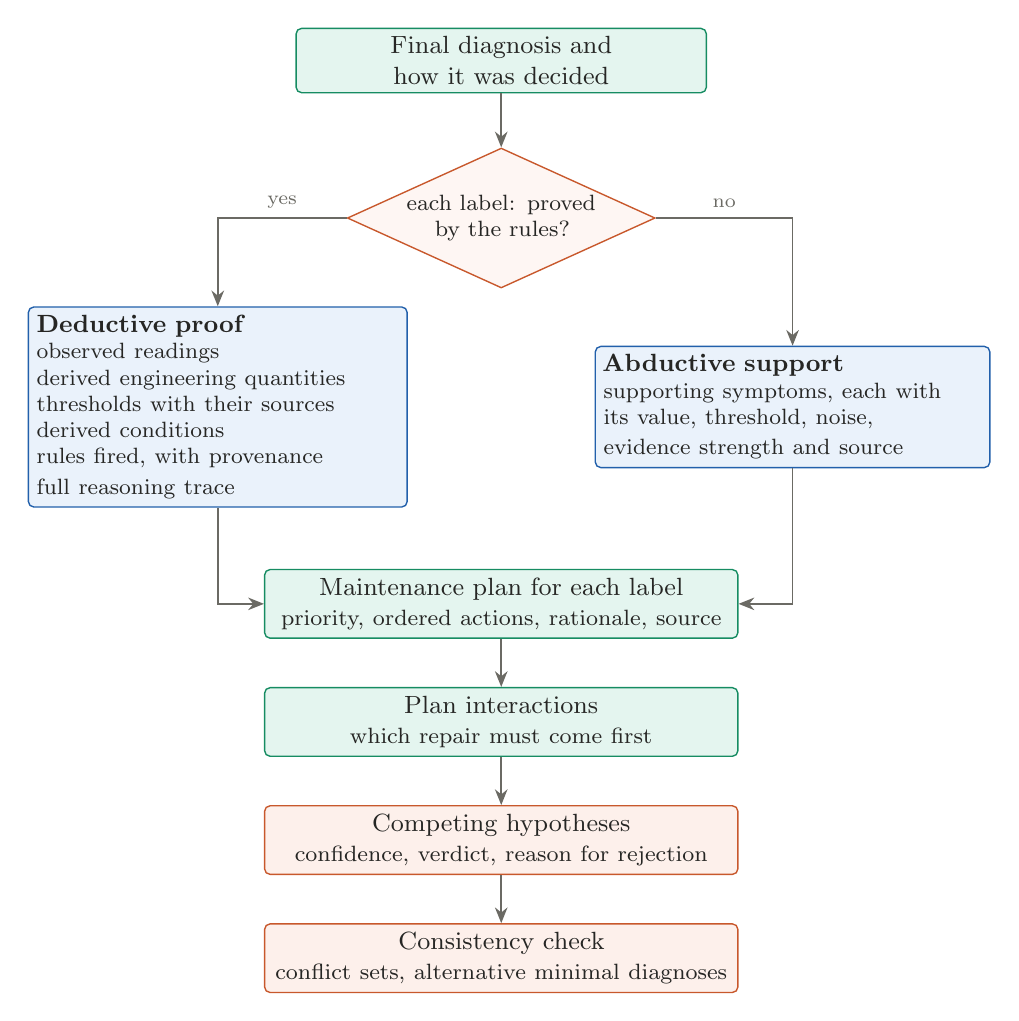
\begin{tikzpicture}[x=1cm, y=1cm]
  \node[out=5cm] (diag) at (4.5,0) {Final diagnosis and how it was decided};
  \node[decision=2.4cm] (dec) at (4.5,-2.0) {each label: proved by the rules?};
  \node[kb=4.6cm, align=left] (proof) at (0.9,-4.4)
    {\textbf{Deductive proof}\\
     \footnotesize observed readings\\
     \footnotesize derived engineering quantities\\
     \footnotesize thresholds with their sources\\
     \footnotesize derived conditions\\
     \footnotesize rules fired, with provenance\\
     \footnotesize full reasoning trace};
  \node[kb=4.8cm, align=left] (abd) at (8.2,-4.4)
    {\textbf{Abductive support}\\
     \footnotesize supporting symptoms, each with\\
     \footnotesize its value, threshold, noise,\\
     \footnotesize evidence strength and source};
  \node[out=5.8cm] (plan) at (4.5,-6.9) {Maintenance plan for each label\\ \footnotesize priority, ordered actions, rationale, source};
  \node[out=5.8cm] (inter) at (4.5,-8.4) {Plan interactions\\ \footnotesize which repair must come first};
  \node[reason=5.8cm] (comp) at (4.5,-9.9) {Competing hypotheses\\ \footnotesize confidence, verdict, reason for rejection};
  \node[reason=5.8cm] (cons) at (4.5,-11.4) {Consistency check\\ \footnotesize conflict sets, alternative minimal diagnoses};

  \draw[flow] (diag) -- (dec);
  \draw[flow] (dec.west) -| node[tag, pos=0.25, above] {yes} (proof.north);
  \draw[flow] (dec.east) -| node[tag, pos=0.25, above] {no} (abd.north);
  \draw[flow] (proof.south) |- (plan.west);
  \draw[flow] (abd.south) |- (plan.east);
  \draw[flow] (plan) -- (inter);
  \draw[flow] (inter) -- (comp);
  \draw[flow] (comp) -- (cons);
\end{tikzpicture}

  \caption{Explanation-generation workflow of the explanation facility.}
  \label{fig:explanation}
\end{figure}

Listing~\ref{lst:why} shows the explanation of a held-out test case in which recirculation at rack A04 is hidden by a top inlet sensor that reads low. The output is reproduced unedited. It shows each of the eight elements that the framework requires of an explanation: observed evidence, derived conditions, rules activated, intermediate reasoning, the diagnosis, competing hypotheses, the reasons for rejecting weaker ones and the recommended action.

\lstinputlisting[language={}, basicstyle=\ttfamily\scriptsize, caption={Unedited output of \texttt{why(h188)}: recirculation hidden by a low-reading sensor.}, label={lst:why}]{listings/why_h188.txt}

% ---------------------------------------------------------------------------
\section{Corrective-Maintenance Planner}
\label{sec:planner}

Every fault class has a plan in \texttt{kb/maintenance.pl}, with a priority, ordered actions, an engineering rationale and a source:
\begin{lstlisting}
maintenance(branch_overload, urgent,
    [ 'Identify the servers on the overloaded phase from the rack power records',
      'Rebalance server power supplies across the three phases',
      'Check for equipment added without a capacity review',
      'Confirm every phase is below 80% of its breaker rating' ],
    'A phase above its continuous rating can trip its breaker and drop every
     server on that circuit.',
    nec_continuous).
\end{lstlisting}
Each plan ends with a verification step that confirms the repair worked, such as re-measuring a temperature or a current. Figure~\ref{fig:maintenance} shows how plans are assembled. A diagnosed label is split into its fault class and entity, and the plan for the class is instantiated for the entity.

\begin{figure}[htbp]
  \centering
  % Figure 7: corrective-maintenance planning workflow.
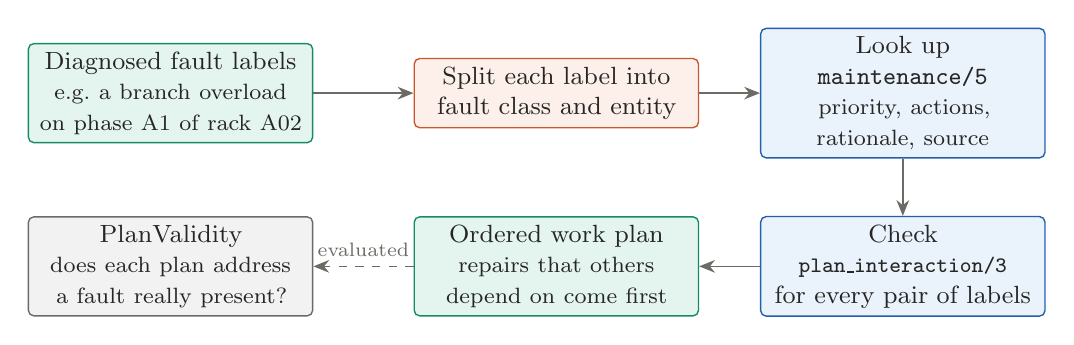
\begin{tikzpicture}[x=1cm, y=1cm]
  \node[out=3.4cm] (lab) at (-0.5,0) {Diagnosed fault labels\\ \footnotesize e.g.\ a branch overload on phase A1 of rack A02};
  \node[reason=3.4cm] (map) at (4.4,0) {Split each label into fault class and entity};
  \node[kb=3.4cm] (kb) at (8.8,0) {Look up \texttt{maintenance/5}\\ \footnotesize priority, actions, rationale, source};
  \node[kb=3.4cm] (int) at (8.8,-2.2) {Check \texttt{\footnotesize plan\_interaction/3} for every pair of labels};
  \node[out=3.4cm] (plan) at (4.4,-2.2) {Ordered work plan\\ \footnotesize repairs that others depend on come first};
  \node[data=3.4cm] (eval) at (-0.5,-2.2) {PlanValidity\\ \footnotesize does each plan address a fault really present?};

  \draw[flow] (lab) -- (map);
  \draw[flow] (map) -- (kb);
  \draw[flow] (kb) -- (int);
  \draw[flow] (int) -- (plan);
  \draw[uses] (plan) -- node[tag, above] {evaluated} (eval);
\end{tikzpicture}

  \caption{Corrective-maintenance planning workflow.}
  \label{fig:maintenance}
\end{figure}

Table~\ref{tab:maintenance} lists the plan issued for every diagnosis. It is generated from the knowledge base, like the rule table.

% Generated by tests/export_latex.pl from the knowledge base. Do not edit by hand.
\begin{footnotesize}
\begin{longtable}{L{2.8cm}L{1.3cm}L{8.2cm}L{2.0cm}}
  \caption{Maintenance-action mapping, generated from \texttt{kb/maintenance.pl}: the corrective plan issued for each diagnosis, in order.}\label{tab:maintenance}\\
  \toprule
  Diagnosis & Priority & Ordered actions & Source \\
  \midrule
  \endfirsthead
  \toprule
  Diagnosis & Priority & Ordered actions & Source \\
  \midrule
  \endhead
  \texttt{crah\_\allowbreak{}fan\_\allowbreak{}failure} & urgent & 1.~Check the fan drive fault log and the motor current \newline 2.~Inspect the motor, belt or coupling, and bearings; repair or replace the failed part \newline 3.~Bring redundant cooling online or raise the output of neighbouring units during the repair \newline 4.~After repair, confirm fan power matches the affinity-law prediction and rack inlets fall below 27 C & \texttt{ashrae\_\allowbreak{}hb\_\allowbreak{}fans} \\
  \texttt{chw\_\allowbreak{}supply\_\allowbreak{}loss} & urgent & 1.~Confirm chilled-water plant status: pumps running and isolation valves open \newline 2.~Compare commanded and actual valve stroke; repair or replace a seized actuator \newline 3.~Vent trapped air from the coil \newline 4.~Confirm water flow matches the valve position and supply air is back at setpoint & \texttt{a4\_\allowbreak{}chw\_\allowbreak{}flow} \\
  \texttt{hot\_\allowbreak{}air\_\allowbreak{}recirculation} & high & 1.~Inspect the rack for missing blanking panels and unsealed cable openings \newline 2.~Check containment doors and roof panels for gaps \newline 3.~Install blanking panels and seal the openings \newline 4.~Re-measure top and middle inlet temperatures to confirm the difference is below 3 K & \texttt{eu\_\allowbreak{}coc\_\allowbreak{}dc} \\
  \texttt{normal} & routine & 1.~No corrective action. Continue routine monitoring. & \texttt{ashrae\_\allowbreak{}tc99\_\allowbreak{}2021} \\
  \texttt{unexplained\_\allowbreak{}abnormality} & high & 1.~Verify the affected sensors before acting \newline 2.~Escalate to a technician for manual investigation & \texttt{closed\_\allowbreak{}world} \\
  \texttt{filter\_\allowbreak{}clogging} & high & 1.~Replace the CRAH air filters \newline 2.~Check the filter differential pressure gauge against a reference \newline 3.~Review the filter replacement interval and recent dust sources such as building work \newline 4.~After replacement, confirm filter pressure drop and fan speed are back to normal & \texttt{a8\_\allowbreak{}filter} \\
  \texttt{server\_\allowbreak{}fan\_\allowbreak{}failure} & high & 1.~Check the server management controller event log for the failed fan module \newline 2.~Migrate or reduce the workload on the server until it is repaired \newline 3.~Hot-swap the failed fan module \newline 4.~Confirm CPU temperature and clock frequency return to normal & \texttt{a9\_\allowbreak{}server\_\allowbreak{}fan} \\
  \texttt{branch\_\allowbreak{}overload} & urgent & 1.~Identify the servers on the overloaded phase from the rack power records \newline 2.~Rebalance server power supplies across the three phases \newline 3.~Check for equipment added without a capacity review \newline 4.~Confirm every phase is below 80\% of its breaker rating & \texttt{nec\_\allowbreak{}continuous} \\
  \texttt{battery\_\allowbreak{}degradation} & high & 1.~Confirm with a capacity discharge test as IEEE Std 1188 recommends \newline 2.~Check battery room temperature and its cooling \newline 3.~Replace weak blocks or the whole string, depending on the test result \newline 4.~Record a new resistance baseline after replacement & \texttt{a11\_\allowbreak{}battery} \\
  \texttt{ups\_\allowbreak{}on\_\allowbreak{}bypass} & urgent & 1.~Read the UPS alarm log to find why it transferred to bypass \newline 2.~Call the UPS service engineer to repair the inverter or rectifier fault \newline 3.~Postpone any upstream electrical work while the load has no battery protection \newline 4.~Return the UPS to double conversion after the repair and confirm normal efficiency & \texttt{a12\_\allowbreak{}ups} \\
  \texttt{sensor\_\allowbreak{}bias} & high & 1.~Check the sensor against a calibrated reference instrument \newline 2.~Check the sensor mounting and position \newline 3.~Recalibrate or replace the sensor \newline 4.~Do not act on readings from this sensor until it is verified & \texttt{a13\_\allowbreak{}neighbour} \\
  \texttt{telemetry\_\allowbreak{}dropout} & high & 1.~Check the monitoring agent, controller and network link for this telemetry group \newline 2.~Restore the data feed \newline 3.~Treat the equipment status as unknown until fresh data arrives \newline 4.~Inspect critical equipment on site if the feed cannot be restored quickly & \texttt{a14\_\allowbreak{}telemetry} \\
  \bottomrule
\end{longtable}
\end{footnotesize}


\paragraph{Plan interactions.} When two diagnoses interact, their plans must be ordered. The verification step of the recirculation plan re-measures the rack's top inlet temperature. If the same rack's top inlet sensor is also diagnosed as biased, that step would rely on a faulty sensor. \texttt{plan\_interaction/3} records such dependencies, and the planner then says to repair the sensor first, as Listing~\ref{lst:why} shows. Similar interactions cover the supply-air sensor, whose reading the cooling-unit plans rely on, and stale telemetry, which leaves any plan for the affected equipment unverifiable.

\paragraph{Plan validity.} Whether each issued plan addresses a fault that is really present is measured as PlanValidity in Chapter~\ref{ch:dataset_and_evaluation}. A plan for a fault that is not present wastes maintenance effort. A missing plan for a fault that is present leaves it unrepaired.

\section*{Generated tables}
\addcontentsline{toc}{section}{Generated tables}

Tables~\ref{tab:thresholds} and~\ref{tab:provenance} are generated from the knowledge base by \texttt{tests/export\_latex.pl}, like Table~\ref{tab:rules}.

% Generated by tests/export_latex.pl from the knowledge base. Do not edit by hand.
\begin{small}
\begin{longtable}{L{4.0cm}L{1.4cm}L{1.5cm}L{3.7cm}L{2.4cm}}
  \caption{Thresholds, generated from \texttt{kb/thresholds.pl}.}\label{tab:thresholds}\\
  \toprule
  Threshold & Value & Unit & Source & Source type \\
  \midrule
  \endfirsthead
  \toprule
  Threshold & Value & Unit & Source & Source type \\
  \midrule
  \endhead
  \texttt{t\_\allowbreak{}inlet\_\allowbreak{}rec\_\allowbreak{}max} & 27.0 & degC & \texttt{ashrae\_\allowbreak{}tc99\_\allowbreak{}2021} & standard \\
  \texttt{t\_\allowbreak{}inlet\_\allowbreak{}rec\_\allowbreak{}min} & 18.0 & degC & \texttt{ashrae\_\allowbreak{}tc99\_\allowbreak{}2021} & standard \\
  \texttt{t\_\allowbreak{}supply\_\allowbreak{}setpoint} & 20.0 & degC & \texttt{a1\_\allowbreak{}supply\_\allowbreak{}setpoint} & assumption \\
  \texttt{t\_\allowbreak{}supply\_\allowbreak{}band} & 2.0 & kelvin & \texttt{a1\_\allowbreak{}supply\_\allowbreak{}setpoint} & assumption \\
  \texttt{row\_\allowbreak{}hot\_\allowbreak{}fraction} & 0.5 & ratio & \texttt{a2\_\allowbreak{}row\_\allowbreak{}fraction} & assumption \\
  \texttt{valve\_\allowbreak{}open\_\allowbreak{}min} & 50.0 & percent & \texttt{a3\_\allowbreak{}valve\_\allowbreak{}open} & assumption \\
  \texttt{chw\_\allowbreak{}flow\_\allowbreak{}ratio\_\allowbreak{}min} & 0.3 & ratio & \texttt{a4\_\allowbreak{}chw\_\allowbreak{}flow} & assumption \\
  \texttt{strat\_\allowbreak{}max} & 3.0 & kelvin & \texttt{a5\_\allowbreak{}stratification} & assumption \\
  \texttt{fan\_\allowbreak{}ratio\_\allowbreak{}min} & 0.5 & ratio & \texttt{a6\_\allowbreak{}fan\_\allowbreak{}ratio} & assumption \\
  \texttt{strat\_\allowbreak{}out\_\allowbreak{}max} & 3.5 & kelvin & \texttt{a7\_\allowbreak{}outlet\_\allowbreak{}strat} & assumption \\
  \texttt{filter\_\allowbreak{}loading\_\allowbreak{}max} & 1.7 & ratio & \texttt{a8\_\allowbreak{}filter} & assumption \\
  \texttt{server\_\allowbreak{}fan\_\allowbreak{}min} & 1000.0 & rpm & \texttt{a9\_\allowbreak{}server\_\allowbreak{}fan} & assumption \\
  \texttt{cpu\_\allowbreak{}hot\_\allowbreak{}min} & 85.0 & degC & \texttt{a10\_\allowbreak{}cpu} & assumption \\
  \texttt{branch\_\allowbreak{}loading\_\allowbreak{}max} & 0.8 & ratio & \texttt{nec\_\allowbreak{}continuous} & standard \\
  \texttt{cell\_\allowbreak{}r\_\allowbreak{}ratio\_\allowbreak{}max} & 1.3 & ratio & \texttt{a11\_\allowbreak{}battery} & assumption \\
  \texttt{ups\_\allowbreak{}eff\_\allowbreak{}bypass\_\allowbreak{}min} & 0.98 & ratio & \texttt{a12\_\allowbreak{}ups} & assumption \\
  \texttt{neighbour\_\allowbreak{}dev\_\allowbreak{}max} & 2.0 & kelvin & \texttt{a13\_\allowbreak{}neighbour} & assumption \\
  \texttt{balance\_\allowbreak{}resid\_\allowbreak{}max} & 0.2 & ratio & \texttt{eq40\_\allowbreak{}uncertainty} & method \\
  \texttt{sample\_\allowbreak{}age\_\allowbreak{}max} & 60.0 & s & \texttt{a14\_\allowbreak{}telemetry} & assumption \\
  \texttt{t\_\allowbreak{}supply\_\allowbreak{}hot\_\allowbreak{}limit} & 22.0 & degC & \texttt{a1\_\allowbreak{}supply\_\allowbreak{}setpoint} & assumption \\
  \texttt{fan\_\allowbreak{}ratio\_\allowbreak{}reduced} & 0.85 & ratio & \texttt{a17\_\allowbreak{}fan\_\allowbreak{}reduced} & assumption \\
  \texttt{t\_\allowbreak{}supply\_\allowbreak{}cold\_\allowbreak{}limit} & 18.0 & degC & \texttt{a1\_\allowbreak{}supply\_\allowbreak{}setpoint} & assumption \\
  \texttt{power\_\allowbreak{}resid\_\allowbreak{}max} & 0.1 & ratio & \texttt{a15\_\allowbreak{}power\_\allowbreak{}balance} & assumption \\
  \texttt{sensor\_\allowbreak{}noise\_\allowbreak{}floor} & 0.15 & kelvin & \texttt{a16\_\allowbreak{}noise} & assumption \\
  \bottomrule
\end{longtable}
\end{small}

% Generated by tests/export_latex.pl from the knowledge base. Do not edit by hand.
\begin{small}
\begin{longtable}{L{3.4cm}L{2.4cm}L{8.2cm}}
  \caption{Provenance of rules and thresholds, generated from \texttt{kb/sources.pl}.}\label{tab:provenance}\\
  \toprule
  Source & Type & Citation or justification \\
  \midrule
  \endfirsthead
  \toprule
  Source & Type & Citation or justification \\
  \midrule
  \endhead
  \texttt{ashrae\_\allowbreak{}tc99\_\allowbreak{}2021} & standard & ASHRAE TC 9.9 (2021). Thermal guidelines for data processing environments (5th ed.). ASHRAE. \\
  \texttt{ashrae\_\allowbreak{}hb\_\allowbreak{}fans} & literature & ASHRAE (2020). 2020 ASHRAE Handbook - HVAC Systems and Equipment, fans chapter. Fan affinity laws. \\
  \texttt{eu\_\allowbreak{}coc\_\allowbreak{}dc} & standard & Acton et al. (2018). 2018 Best Practice Guidelines for the EU Code of Conduct on Data Centre Energy Efficiency, v9.1.0 (European Commission JRC), practice 5.1.4. \\
  \texttt{a1\_\allowbreak{}supply\_\allowbreak{}setpoint} & assumption & Design assumption: CRAH supply-air setpoint 20 C with a 2 K tolerance band. \\
  \texttt{a2\_\allowbreak{}row\_\allowbreak{}fraction} & assumption & Engineering assumption: overheating at half or more of the racks indicates a row-level cause. \\
  \texttt{a3\_\allowbreak{}valve\_\allowbreak{}open} & assumption & Engineering assumption: a valve open 50\% or more should produce a measurable water temperature rise. \\
  \texttt{a4\_\allowbreak{}chw\_\allowbreak{}flow} & assumption & Engineering assumption: measured water flow below 30\% of the valve-characteristic prediction means chilled-water supply is lost. \\
  \texttt{a5\_\allowbreak{}stratification} & assumption & Engineering assumption: a top-to-middle inlet difference above 3 K indicates hot-air recirculation. \\
  \texttt{a6\_\allowbreak{}fan\_\allowbreak{}ratio} & assumption & Engineering assumption: fan power below 50\% of the affinity-law prediction means the fan is not moving air. \\
  \texttt{closed\_\allowbreak{}world} & method & Closed-world assumption: normal operation is concluded when no fault rule fires and all inlets are within the envelope. \\
  \texttt{nec\_\allowbreak{}continuous} & standard & NFPA (2023). NFPA 70 National Electrical Code, continuous-load rule: 80\% of breaker rating. Local codes may differ. \\
  \texttt{a7\_\allowbreak{}outlet\_\allowbreak{}strat} & assumption & Engineering assumption: a top-to-bottom outlet difference above 3.5 K confirms recirculation. Normal racks stay below 3 K. \\
  \texttt{a8\_\allowbreak{}filter} & assumption & Engineering assumption: filter resistance 1.7 times its clean value calls for replacement (check against manufacturer final-resistance data). \\
  \texttt{a9\_\allowbreak{}server\_\allowbreak{}fan} & assumption & Engineering assumption: a server fan below 1000 rpm has failed. The controller never runs it below about 5400 rpm. \\
  \texttt{a10\_\allowbreak{}cpu} & assumption & Engineering assumption: CPU temperature of 85 C or more, 10 K below the 95 C throttling limit, confirms lost server cooling. \\
  \texttt{a11\_\allowbreak{}battery} & assumption & Engineering assumption: cell internal resistance 30\% above its baseline indicates degradation (check against IEEE Std 1188 and manufacturer guidance). \\
  \texttt{a12\_\allowbreak{}ups} & assumption & Engineering assumption: UPS efficiency of 0.98 or more is only reached on static bypass. Double conversion runs at about 0.95. \\
  \texttt{a13\_\allowbreak{}neighbour} & assumption & Engineering assumption: a temperature sensor more than 2 K from the median of sensors that see the same air is suspect (Stage 4 Eq. 41). \\
  \texttt{eq40\_\allowbreak{}uncertainty} & method & Residual threshold from uncertainty propagation, Stage 4 Eqs. 39 and 40, with a coverage factor of about 3. \\
  \texttt{a14\_\allowbreak{}telemetry} & assumption & Engineering assumption: a sample older than 60 s is stale, given a polling interval of about 30 s. \\
  \texttt{eq18\_\allowbreak{}mixing} & method & Physical constraint from the mixing model, Stage 4 Eq. 18: the top inlet cannot be colder than the middle inlet. \\
  \texttt{a15\_\allowbreak{}power\_\allowbreak{}balance} & assumption & Engineering assumption: metered rack power and the sum of its six phase currents agree within 10\% when both meters are healthy (Stage 4 Eq. 42). \\
  \texttt{a16\_\allowbreak{}noise} & assumption & Engineering assumption: temperature-sensor noise is at least 0.15 K (typical datasheet accuracy). Higher noise is estimated from the spread of middle inlets, which all see the same supply air. \\
  \texttt{a17\_\allowbreak{}fan\_\allowbreak{}reduced} & assumption & Engineering assumption: fan power below 85\% of the affinity-law prediction shows a partial failure such as belt slip. Healthy fans stay within 5\%. \\
  \bottomrule
\end{longtable}
\end{small}


\chapter{Dataset, Experimental Methodology and Evaluation}
\label{ch:dataset_and_evaluation}

This chapter describes the data the expert system was tested on (Sections~\ref{sec:dataset} and~\ref{sec:testcases}), how the experiments were designed and validated (Sections~\ref{sec:design} and~\ref{sec:validation}), how performance was measured (Section~\ref{sec:metrics}) and what the results show (Sections~\ref{sec:results} and~\ref{sec:sensitivity}). Every table of results in this chapter is generated by the test code from the current knowledge base and datasets, so the numbers can be reproduced exactly (Chapter~\ref{ch:software_and_reproducibility}).

% ---------------------------------------------------------------------------
\section{Dataset and Data Dictionary}
\label{sec:dataset}

\subsection{Data origin}

\textbf{Every test case in this project is synthetic.} No measured fault data from a real data centre were available, and no value in the dataset is presented as a real measurement. The project framework requires four kinds of information to be kept apart, and they are kept apart as follows:

\begin{itemize}
  \item \textbf{Measured data:} none.
  \item \textbf{Synthetic test cases:} generated by a physics simulator, or written by hand for four smoke tests. Every case carries the origin \texttt{synthetic} in its \texttt{case/3} fact.
  \item \textbf{Engineering assumptions:} recorded as sources of type \texttt{assumption} in the knowledge base (Table~\ref{tab:provenance}), and listed for the simulator in Table~\ref{tab:sim-assumptions}.
  \item \textbf{Literature-supported rules:} rules whose source is of type \texttt{standard} or \texttt{literature}.
\end{itemize}

\subsection{The simulator}

The test cases were generated by a steady-state simulator of the row, written in Python with only the standard library. It implements the engineering model of Section~\ref{sec:maths}. Each case is built in four steps:

\begin{enumerate}
  \item \textbf{Workload.} The row load is drawn as low, nominal or high, at mean utilisations of 10 to 20\%, 40 to 60\% or 80 to 90\%. Each rack varies around the row value and each server around its rack.
  \item \textbf{Fault injection into the physics.} A fault changes a physical parameter, never a reading directly. A fan failure, for example, reduces the airflow the fan delivers, and every temperature then follows from the physics. Table~\ref{tab:fault-params} lists the parameter changed for each fault.
  \item \textbf{Steady-state solution.} The coupled server, rack, cooling-unit and coil equations are solved by damped fixed-point iteration. The cooling-unit fan follows the airflow demand of the servers, and the valve controller finds the smallest opening that holds the 20\,\textdegree C setpoint.
  \item \textbf{Sensor layer.} Sensor bias, Gaussian measurement noise, frozen readings for stale telemetry and randomly missing readings are applied last.
\end{enumerate}

Because faults act on the physics, their symptoms arise as consequences rather than being written in. The diagnostic rules are therefore tested against behaviour they were not built from, which is what exposed the three knowledge-base errors described in Section~\ref{sec:acquisition}.

\begin{table}[htbp]
  \centering
  \small
  \caption{Physical parameter changed for each injected fault.}
  \label{tab:fault-params}
  \begin{tabular}{L{3.2cm}L{6.4cm}L{2.2cm}L{2.2cm}}
    \toprule
    Fault & Parameter changed & Clear range & Borderline range \\
    \midrule
    $F_1$ CRAH fan failure & Airflow fraction delivered; fan power over prediction & 0 to 0.1; 0.05 to 0.15 & 0.3 to 0.5; 0.4 to 0.6 \\
    $F_2$ chilled-water loss & Fraction of design water flow available & 0.02 to 0.2 & 0.25 to 0.4 \\
    $F_3$ filter clogging & Filter loading ratio, Equation E27 & 3 to 6 & 1.8 to 2.5 \\
    $F_4$ recirculation & Extra recirculation fraction at the top of one rack & 0.25 to 0.5 & 0.12 to 0.2 \\
    $F_5$ server fan failure & Server airflow and reported fan speed near zero & -- & -- \\
    $F_6$ branch overload & Phase 1 share of feed A, set for a target current & 27 to 30\,A & 24.5 to 26.5\,A \\
    $F_7$ battery degradation & Cell resistance ratio, with low float voltage & 1.5 to 2.5 & 1.2 to 1.4 \\
    $F_8$ UPS on bypass & Mode flag; efficiency rises to 0.99 & -- & -- \\
    $S_1$ sensor bias & Offset on one inlet or supply-air sensor & 3 to 8\,K & -- \\
    $S_2$ telemetry dropout & One telemetry group frozen, sample age 300 to 1800\,s & -- & -- \\
    \bottomrule
  \end{tabular}
\end{table}

\begin{table}[htbp]
  \centering
  \small
  \caption{Main simulator assumptions.}
  \label{tab:sim-assumptions}
  \begin{tabular}{L{3.8cm}L{5.4cm}L{4.8cm}}
    \toprule
    Assumption & Value & Reason \\
    \midrule
    Server power & 0.40\,kW idle, 0.90\,kW at full load, 55\% in the CPU & Equation E1; a typical two-socket server (to verify) \\
    Server airflow & 0.055\,kg/s at nominal fan speed & Gives a 13 to 16\,K rise across a server \\
    CPU throttling & Clock reduced to keep the CPU at or below 95\,\textdegree C & Vendor limits vary (to verify) \\
    Cooling-unit fan control & Supplies 10\% more air than the servers demand & Common practice to limit recirculation \\
    Coil heat transfer & 15\,kW/K air side; 10\,kW/K water side at 3.2\,kg/s, scaling with flow to the power 0.8 & Gives a 5 to 7\,K water temperature rise in normal operation \\
    Airflow shortfall & 40\% drawn from the hot aisle, 60\% from room air at 25\,\textdegree C & Without it a fan failure has no steady state \\
    Power distribution & Two feeds per rack sharing the load equally & Standard 2N practice \\
    Measurement noise & 0.15\,K on air temperatures; 1\% on power and current & Typical sensor accuracy (to verify) \\
    Time & Steady state only & A limitation: transients are not modelled \\
    \bottomrule
  \end{tabular}
\end{table}

\subsection{Data dictionary}

The variables, units and sensors are defined in Table~\ref{tab:variables}. Each case has about 460 readings: nine for the cooling unit, six for each rack, one current for each of the six phase circuits of each rack, three for each of the 120 servers, six for the UPS and battery, and one sample age for each telemetry group. The simulator writes every dataset in three forms: Prolog facts for the expert system, a CSV file in long format with units for analysis outside Prolog, and a JSON file holding the hidden ground truth of each case, such as the injected severities.

\subsection{Datasets}

Four datasets were used (Table~\ref{tab:datasets}). The calibration and held-out splits have the same composition but different random seeds. A fixed seed always reproduces the same cases.

\begin{table}[htbp]
  \centering
  \small
  \caption{Datasets.}
  \label{tab:datasets}
  \begin{tabular}{L{3.0cm}L{2.0cm}L{2.2cm}L{6.8cm}}
    \toprule
    Dataset & Cases & Seed & Use \\
    \midrule
    Smoke tests & 4 & -- & Hand-written cases for the explanation demonstrations \\
    Calibration & 255 & 20261020 & Checking thresholds and signatures during development \\
    Held-out & 255 & 777 & Reported performance; never used to adjust anything \\
    Sensitivity sweeps & 24 $\times$ 60 & 4242 to 4545 & Sensitivity to noise, missing data, multiple faults and sensor bias \\
    \bottomrule
  \end{tabular}
\end{table}

% ---------------------------------------------------------------------------
\section{Test Cases}
\label{sec:testcases}

The calibration and held-out splits each contain seven categories, which together cover the eight test categories that the project framework requires (Table~\ref{tab:test-categories}). Test~H, explanation and maintenance, is assessed on every case through ExplainabilityRate and PlanValidity, and demonstrated in full by the explanation traces of Section~\ref{sec:explanation}.

\begin{table}[htbp]
  \centering
  \small
  \caption{Test categories and the framework tests they cover.}
  \label{tab:test-categories}
  \begin{tabular}{L{2.6cm}L{1.0cm}L{1.6cm}L{8.8cm}}
    \toprule
    Category & Cases & Test & Contents \\
    \midrule
    Normal & 30 & A & 10 cases each at low, nominal and high load \\
    Single fault & 120 & B, C, D & 15 cases of each physical fault $F_1$ to $F_8$ \\
    Instrumentation & 30 & E & 15 sensor-bias and 15 telemetry-dropout cases \\
    Multiple & 30 & F & 6 cases of each combination in Table~\ref{tab:interactions} \\
    Incomplete & 15 & G & A random single fault or normal case with 15\% of readings removed \\
    High noise & 15 & G & A random single fault with five times the nominal sensor noise \\
    Borderline & 15 & G & Fault severities near or below the detection thresholds, and high-load normal cases \\
    All categories & 255 & H & Explanation and maintenance plan for every diagnosis \\
    \bottomrule
  \end{tabular}
\end{table}

The borderline category deliberately includes faults injected below the detection thresholds. Its exact-match score is therefore expected to be low, and it is reported to measure how gracefully detection degrades, not as a target to maximise.

% ---------------------------------------------------------------------------
\section{Experimental Design}
\label{sec:design}

Figure~\ref{fig:evaluation} shows the experimental workflow. Three design decisions protect the results against optimistic bias.

\begin{figure}[htbp]
  \centering
  % Figure 8: experimental and evaluation workflow.
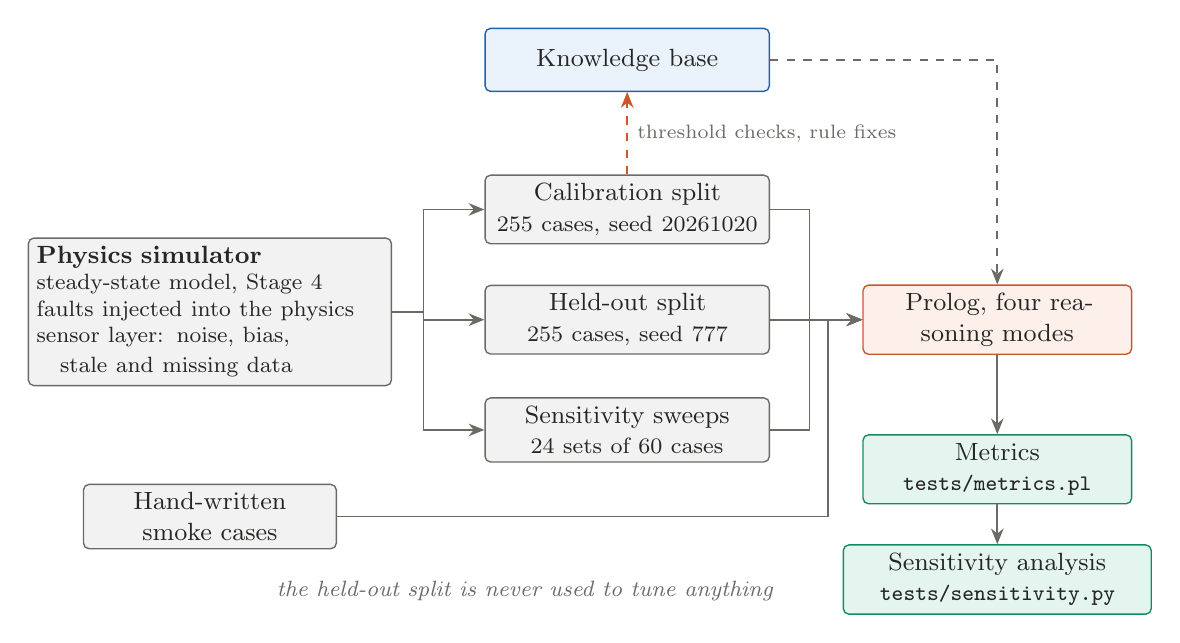
\begin{tikzpicture}[x=1cm, y=1cm]
  \node[data=4.4cm, align=left] (sim) at (0.6,0)
    {\textbf{Physics simulator}\\
     \footnotesize steady-state model, Stage 4\\
     \footnotesize faults injected into the physics\\
     \footnotesize sensor layer: noise, bias,\\
     \footnotesize \quad stale and missing data};
  \node[data=3cm] (hand) at (0.6,-2.6) {Hand-written smoke cases};

  \node[data=3.4cm] (cal) at (5.9,1.3) {Calibration split\\ \footnotesize 255 cases, seed 20261020};
  \node[data=3.4cm] (hold) at (5.9,-0.1) {Held-out split\\ \footnotesize 255 cases, seed 777};
  \node[data=3.4cm] (swp) at (5.9,-1.5) {Sensitivity sweeps\\ \footnotesize 24 sets of 60 cases};

  \node[reason=3.2cm] (pl) at (10.6,-0.1) {Prolog, four reasoning modes};
  \node[out=3.2cm] (met) at (10.6,-2.0) {Metrics\\ \footnotesize \texttt{tests/metrics.pl}};
  \node[out=3.7cm] (sen) at (10.6,-3.4) {Sensitivity analysis\\ \footnotesize \texttt{tests/sensitivity.py}};
  \node[kb=3.4cm] (kb) at (5.9,3.2) {Knowledge base};

  \draw[flow] (sim.east) -- ++(0.4,0) |- (cal.west);
  \draw[flow] (sim.east) -- ++(0.4,0) |- (hold.west);
  \draw[flow] (sim.east) -- ++(0.4,0) |- (swp.west);
  \draw[flow] (hand.east) -- (8.45,-2.6) |- (pl.west);
  \draw[flow] (cal.east) -- ++(0.5,0) |- (pl.west);
  \draw[flow] (hold) -- (pl);
  \draw[flow] (swp.east) -- ++(0.5,0) |- (pl.west);
  \draw[flow] (pl) -- (met);
  \draw[flow] (met) -- (sen);
  \draw[uses] (kb.east) -| (pl.north);
  \draw[feedback] (cal.north) -- node[tag, right] {threshold checks, rule fixes} (kb.south);
  \node[note] at (4.6,-3.55) {the held-out split is never used to tune anything};
\end{tikzpicture}

  \caption{Experimental and evaluation workflow, with the calibration and held-out splits kept apart.}
  \label{fig:evaluation}
\end{figure}

\paragraph{Calibration and held-out splits.} Thresholds were set from engineering reasoning and then checked against the calibration split, by profiling each signature in normal and fault cases. The held-out split was generated afterwards with a different seed and was never used to choose or adjust anything. Its results are the reported performance.

\paragraph{Faults in the physics, not the readings.} Because the simulator injects faults into the physical model, the knowledge base cannot simply reproduce the generator's rules. Symptoms that the knowledge base did not anticipate appear in the data, as the three errors found during development show.

\paragraph{Four configurations on identical data.} The four reasoning configurations of Section~\ref{sec:inference} run on exactly the same cases, so differences between them are due to the reasoning alone. This comparison is the ablation study that the framework asks for.

Reasoning time is measured as wall-clock time per case, after a warm-up pass and with the symptom cache cleared for each case, so that every configuration pays the full cost of its own evidence computation.

% ---------------------------------------------------------------------------
\section{Validation}
\label{sec:validation}

Verification asks whether the system implements its design correctly. Validation asks whether the design is right for the problem. Both were addressed at several levels:

\begin{itemize}
  \item \textbf{Equations against physics.} The simulator's normal cases were checked against independent hand calculations. A 78\,kW row needs about 4.9\,m$^3$/s of air at a 13\,K rise, and the fan figures imply a plausible pressure rise of about 225\,Pa. The coil model was tuned so that normal operation gives the 5 to 7\,K water temperature rise of real chilled-water coils.
  \item \textbf{Rules against simulated physics.} Each new rule was first run against the calibration split. Rules that disagreed with the physics were revised rather than the data, which exposed the three errors of Section~\ref{sec:acquisition}.
  \item \textbf{Generalisation.} The held-out split measures performance on cases that played no part in development. Held-out accuracy is slightly higher than calibration accuracy for every configuration (Tables~\ref{tab:modes-holdout} and~\ref{tab:modes-calibration}), which makes overfitting to the calibration split unlikely. Both splits come from the same simulator, however, so this tests generalisation across cases of one model, not to a different system. Section~\ref{sec:mismatch} tests robustness to the model itself.
  \item \textbf{Explanations.} Explanation traces were inspected for representative cases of every category. The trace of Listing~\ref{lst:why} shows each element that the framework requires.
  \item \textbf{Regression.} The four smoke cases and both splits are rerun after every change to the knowledge base.
\end{itemize}

The main limitation of this validation is that both the knowledge base and the simulator rest on the same engineering model. Agreement between them shows that the reasoning is consistent with the model, not that the model is consistent with a real data centre. Section~\ref{sec:mismatch} measures how much the results depend on the model being exactly right, by regenerating the held-out cases with deliberately changed physics. Validation on measured data remains future work (Chapter~\ref{ch:conclusion}).

% ---------------------------------------------------------------------------
\section{Metrics}
\label{sec:metrics}

The metrics follow Section~\ref{sec:maths}. Because a case can contain several faults, each metric is counted as follows:

\begin{itemize}
  \item \textbf{Exact match} is the share of cases whose predicted set of fault labels equals the true set exactly. A label names both the fault and the affected entity, so diagnosing recirculation at the wrong rack counts as wrong.
  \item \textbf{Coverage} is the share of cases in which every true fault was predicted, whether or not extra faults were predicted too.
  \item \textbf{Precision, recall and F1-score} are computed for each fault class from label-level counts: a predicted label that matches a true label is a true positive. Macro averages are taken over the eleven classes.
  \item \textbf{Class accuracy} is the framework's Equation~\eqref{eq:metrics} at case level: for each class, the share of cases in which the presence or absence of that class was predicted correctly. Its mean over the classes is reported.
  \item \textbf{ExplainabilityRate} is the share of cases in which every reported label has a justification, meaning a deductive proof, a clearly present supporting symptom or a hit conflict set, together with a maintenance plan and sourced thresholds. The system only reports a label for one of these reasons, so this rate cannot fall below 100\%. It confirms that every output is traceable, not that the explanation is the real reason for the output. Explanation fidelity, below, tests that.
  \item \textbf{Explanation fidelity} removes the observations an explanation cites and diagnoses the case again (Section~\ref{sec:fidelity}). Unlike ExplainabilityRate, it can fail.
  \item \textbf{PlanValidity} is the share of issued maintenance plans that address a fault really present. A routine plan counts as valid only for a truly normal case. One plan is issued per label, and a plan counts as valid when its label is correct, so PlanValidity is in effect label-level precision. It does not test whether a plan's actions are the right ones. That rests on the plans' sources and verification steps (Section~\ref{sec:planner}), and ideally on review by a practitioner.
  \item \textbf{Reasoning time} is the mean and maximum wall-clock time per case.
\end{itemize}

Confidence scores are used only to rank hypotheses. No probability is claimed, so probabilistic metrics such as calibration curves are not reported.

% ---------------------------------------------------------------------------
\section{Results}
\label{sec:results}

\subsection{Overall performance}

Table~\ref{tab:modes-holdout} gives the held-out results of the four configurations, and Table~\ref{tab:modes-calibration} the calibration results for comparison. Each exact-match rate is given with its Wilson 95\% confidence interval. Because all four configurations diagnose the same cases, they are compared pairwise with an exact McNemar test on the cases where they disagree (Table~\ref{tab:significance-holdout}).

% Generated by tests/metrics_latex.pl. Do not edit by hand.
\begin{table}[htbp]
  \centering
  \footnotesize
  \setlength{\tabcolsep}{4pt}
  \caption{Comparison of reasoning modes, held-out split (255 cases). Class acc.: mean class accuracy. Explain.: ExplainabilityRate. Plan val.: PlanValidity.}
  \label{tab:modes-holdout}
  \begin{tabular}{L{3.4cm}rrrrrrr}
  \toprule
  Mode & Exact & Coverage & Macro F1 & Class acc. & Mean ms & Explain. & Plan val. \\
  \midrule
  Deductive only & 91.0\% & 95.7\% & 0.924 & 98.6\% & 0.22 & 100.0\% & 85.1\% \\
  Deductive + abductive & 94.5\% & 96.1\% & 0.958 & 99.0\% & 1.09 & 100.0\% & 94.2\% \\
  Deductive + consistency-based & 93.3\% & 97.3\% & 0.950 & 99.0\% & 1.03 & 100.0\% & 91.4\% \\
  Complete system & 93.7\% & 96.5\% & 0.954 & 99.0\% & 1.16 & 100.0\% & 92.9\% \\
  \bottomrule
  \end{tabular}
\end{table}

% Generated by tests/metrics_latex.pl. Do not edit by hand.
\begin{table}[htbp]
  \centering
  \footnotesize
  \setlength{\tabcolsep}{4pt}
  \caption{Comparison of reasoning modes, calibration split (255 cases). 95\% CI: Wilson confidence interval of the exact-match rate. Explain.: ExplainabilityRate. Plan val.: PlanValidity.}
  \label{tab:modes-calibration}
  \begin{tabular}{L{2.9cm}rrrrrrrr}
  \toprule
  Mode & Exact & 95\% CI & Coverage & Macro F1 & Mean ms & Max ms & Explain. & Plan val. \\
  \midrule
  Deductive only & 90.2\% & 85.9--93.3 & 95.3\% & 0.925 & 0.18 & 0.68 & 100.0\% & 86.7\% \\
  Deductive + abductive & 93.3\% & 89.6--95.8 & 94.5\% & 0.954 & 0.95 & 2.52 & 100.0\% & 94.4\% \\
  Deductive + consistency-based & 91.8\% & 87.7--94.6 & 95.3\% & 0.942 & 0.84 & 2.48 & 100.0\% & 91.6\% \\
  Complete system & 93.3\% & 89.6--95.8 & 95.3\% & 0.952 & 0.96 & 3.20 & 100.0\% & 93.8\% \\
  \bottomrule
  \end{tabular}
\end{table}

% Generated by tests/metrics_latex.pl. Do not edit by hand.
\begin{table}[htbp]
  \centering
  \small
  \caption{Paired comparison of reasoning modes, held-out split: exact two-sided McNemar test on the cases where the two modes disagree. Only A: cases the first mode gets right and the second wrong. Holm: $p$ adjusted for the six comparisons by Holm's method. Bold: below 0.05.}
  \label{tab:significance-holdout}
  \begin{tabular}{L{3.6cm}L{3.6cm}rrrr}
  \toprule
  Mode A & Mode B & Only A & Only B & $p$ & Holm \\
  \midrule
  Deductive only & Deductive + abductive & 2 & 11 & \textbf{0.022} & 0.135 \\
  Deductive only & Deductive + consistency-based & 2 & 8 & 0.109 & 0.461 \\
  Deductive only & Complete system & 3 & 10 & 0.092 & 0.461 \\
  Deductive + abductive & Deductive + consistency-based & 5 & 2 & 0.453 & 1.000 \\
  Deductive + abductive & Complete system & 2 & 0 & 0.500 & 1.000 \\
  Deductive + consistency-based & Complete system & 2 & 3 & 1.000 & 1.000 \\
  \bottomrule
  \end{tabular}
\end{table}


Four findings stand out.

\begin{enumerate}
  \item \textbf{Every configuration is accurate on the core categories.} All four diagnose every normal, single-fault and instrumentation case of the held-out split correctly (Table~\ref{tab:categories-holdout}). Over five held-out seeds, they miss 3 to 6 of the 900 such cases (Section~\ref{sec:seeds}).
  \item \textbf{Abduction gives the largest gain.} Adding abduction raises exact-match accuracy from 91.0\% to 94.5\%. It corrects 11 cases that deduction gets wrong and loses 2, a significant difference ($p = 0.022$). The gain comes almost entirely from the imperfect-evidence categories, where parsimony removes spurious findings. On this split, the complete system's gain over deduction is not significant ($p = 0.092$), although it is on the calibration split ($p = 0.039$) and over five seeds.
  \item \textbf{One split cannot separate the model-based configurations; five seeds can.} On the held-out split their exact-match rates differ by two to five cases, their confidence intervals overlap, and no pairwise difference between them approaches significance ($p \ge 0.45$). Pooled over five held-out seeds, every pairwise difference is significant, and deductive + abductive reasoning is the most accurate configuration (Section~\ref{sec:seeds}). Consistency checking is the only mode that catches the smallest supply-sensor bias in the calibration split, and it refuses explanations that leave a violated relation unexplained. Under heavy noise, however, it occasionally takes a chance violation of the power balance at face value and reports a meter fault.
  \item \textbf{Every output is traceable, and the explanations are faithful.} ExplainabilityRate is 100\% in every configuration, as it must be by construction. The fidelity test, which can fail, finds that removing the evidence an explanation cites removes the diagnosis in 96 to 100\% of cases (Section~\ref{sec:fidelity}). Reasoning takes about 1\,ms per case.
\end{enumerate}

% Generated by tests/metrics_latex.pl. Do not edit by hand.
\begin{table}[htbp]
  \centering
  \small
  \caption{Exact matches by test category and reasoning mode, held-out split.}
  \label{tab:categories-holdout}
  \begin{tabular}{L{3.2cm}L{1.0cm}L{1.0cm}rrrr}
  \toprule
  Category & Test & Cases & Deductive & Ded.\ + abd. & Ded.\ + cons. & Complete \\
  \midrule
  Normal operation & A & 30 & 30 & 30 & 30 & 30 \\
  Single faults & B--D & 120 & 120 & 120 & 120 & 120 \\
  Instrumentation & E & 30 & 30 & 30 & 30 & 30 \\
  Multiple faults & F & 30 & 30 & 29 & 30 & 29 \\
  Incomplete evidence & G & 15 & 13 & 14 & 14 & 14 \\
  High noise & G & 15 & 3 & 9 & 5 & 7 \\
  Borderline & G & 15 & 6 & 9 & 9 & 9 \\
  \bottomrule
  \end{tabular}
\end{table}


\subsection{Variability across seeds}
\label{sec:seeds}

The held-out split is one random draw of 255 cases. To measure how much the results depend on that draw, four more held-out splits were generated with the same design and the seeds 1001, 2002, 3003 and 4004. None of them was used to choose anything. Table~\ref{tab:seeds} gives the exact match of each configuration on each seed, and pooled over all 1275 cases. They are generated by \texttt{tests/seeds.py}.

% Generated by tests/seeds.py. Do not edit by hand.
\begin{table}[htbp]
  \centering
  \footnotesize
  \setlength{\tabcolsep}{4pt}
  \caption{Exact match on five held-out splits of 255 cases with different seeds. Seed 777 is the held-out split reported in Table~\ref{tab:modes-holdout}. SD: sample standard deviation over the five seeds. Pooled: all 1275 cases, with the Wilson 95\% confidence interval.}
  \label{tab:seeds}
  \begin{tabular}{L{5.0cm}rrrrrrrc}
  \toprule
  Mode & 777 & 1001 & 2002 & 3003 & 4004 & Mean & SD & Pooled (95\% CI) \\
  \midrule
  Deductive only & 91.0 & 90.6 & 92.2 & 91.4 & 89.0 & 90.8 & 1.2 & 90.8 (89.1--92.3) \\
  Deductive + abductive & 94.5 & 94.9 & 94.1 & 91.0 & 93.3 & 93.6 & 1.6 & 93.6 (92.1--94.8) \\
  Deductive + consistency-based & 93.3 & 91.4 & 92.5 & 90.2 & 92.2 & 91.9 & 1.2 & 91.9 (90.3--93.3) \\
  Complete system & 93.7 & 93.7 & 93.3 & 90.6 & 92.9 & 92.9 & 1.3 & 92.9 (91.3--94.2) \\
  \bottomrule
  \end{tabular}
\end{table}

\begin{table}[htbp]
  \centering
  \small
  \caption{Paired comparison of reasoning modes pooled over the five held-out seeds (1275 cases): exact two-sided McNemar test on the cases where the two modes disagree. Holm: $p$ adjusted for the six comparisons by Holm's method. Bold: below 0.05.}
  \label{tab:seeds-significance}
  \begin{tabular}{L{3.9cm}L{3.9cm}rrrr}
  \toprule
  Mode A & Mode B & Only A & Only B & $p$ & Holm \\
  \midrule
  Deductive only & Deductive + abductive & 17 & 52 & \textbf{\textless\,0.001} & \textbf{\textless\,0.001} \\
  Deductive only & Deductive + consistency-based & 14 & 28 & \textbf{0.044} & 0.071 \\
  Deductive only & Complete system & 21 & 47 & \textbf{0.002} & \textbf{0.009} \\
  Deductive + abductive & Deductive + consistency-based & 29 & 8 & \textbf{0.001} & \textbf{0.004} \\
  Deductive + abductive & Complete system & 9 & 0 & \textbf{0.004} & \textbf{0.012} \\
  Deductive + consistency-based & Complete system & 8 & 20 & \textbf{0.036} & 0.071 \\
  \bottomrule
  \end{tabular}
\end{table}


The standard deviation across seeds is 1.2 to 1.6 percentage points. That is the same size as the differences between the model-based configurations on any one split, which is why one split cannot separate them. The order is stable where it matters most. On every seed, deductive + abductive reasoning is ahead of the complete system, and the complete system is ahead of deductive + consistency-based reasoning. Deduction alone is last on four seeds, but on seed 3003 it is narrowly first, which shows how much a single split can mislead.

Pooling the paired cases gives the statistical power that one split lacks (Table~\ref{tab:seeds-significance}). Every pairwise difference is then significant. Deductive + abductive reasoning is the most accurate configuration, at 93.6\%. The complete system is never right where deductive + abductive reasoning is wrong, and is wrong in 9 cases where it is right. In each of the 9, it keeps the correct fault and adds a false sensor fault, and 8 of them are high-noise cases. On these data, the consistency check therefore costs more exact matches under noise than it gains. Its benefits show in the controlled experiments, such as detecting the smallest sensor biases (Section~\ref{sec:sensitivity}). Graded consistency checking (Section~\ref{sec:future}) is the change most likely to remove its cost.

The core categories are not perfect on every seed either. Over the five seeds, 3 to 6 of the 900 normal, single-fault and instrumentation cases are misdiagnosed, depending on the configuration. The perfect score on seed 777 is therefore partly the luck of one draw.

\subsection{Results by fault class}

Table~\ref{tab:classes} gives the per-class results of the complete system and Table~\ref{tab:confusion} its confusion matrix. Every single-label case of the held-out split is diagnosed correctly: the confusion matrix is diagonal. The errors that remain occur in the multiple-fault and imperfect-evidence categories, and show in two classes. Sensor bias has a precision of 0.656, because 11 sensor faults were reported that were not present, mostly in high-noise cases. Normal has a precision of 0.829, because seven faulty cases were reported as normal, mostly borderline faults injected below the detection thresholds. The class-accuracy column should be read with care. Each class is absent from most cases, so true negatives dominate it: sensor bias still has a class accuracy of 96.5\% despite its precision of 0.656. Precision, recall and F1-score are the informative measures.

% Generated by tests/metrics_latex.pl. Do not edit by hand.
\begin{table}[htbp]
  \centering
  \small
  \caption{Per-class results of the complete system, held-out split. Counts are of fault labels; class accuracy is at case level (Equation~\eqref{eq:metrics}).}
  \label{tab:classes}
  \begin{tabular}{L{4.2cm}rrrrrrr}
  \toprule
  Class & TP & FP & FN & Precision & Recall & F1 & Class acc. \\
  \midrule
  $F_N$ normal & 34 & 7 & 0 & 0.829 & 1.000 & 0.907 & 97.3\% \\
  $F_1$ CRAH fan failure & 27 & 1 & 0 & 0.964 & 1.000 & 0.982 & 99.6\% \\
  $F_2$ chilled-water loss & 23 & 0 & 0 & 1.000 & 1.000 & 1.000 & 100.0\% \\
  $F_3$ filter clogging & 25 & 0 & 3 & 1.000 & 0.893 & 0.943 & 98.8\% \\
  $F_4$ recirculation & 36 & 2 & 2 & 0.947 & 0.947 & 0.947 & 98.4\% \\
  $F_5$ server fan failure & 24 & 0 & 0 & 1.000 & 1.000 & 1.000 & 100.0\% \\
  $F_6$ branch overload & 23 & 0 & 2 & 1.000 & 0.920 & 0.958 & 99.2\% \\
  $F_7$ battery degradation & 25 & 0 & 2 & 1.000 & 0.926 & 0.962 & 99.2\% \\
  $F_8$ UPS on bypass & 23 & 0 & 0 & 1.000 & 1.000 & 1.000 & 100.0\% \\
  $S_1$ sensor bias & 21 & 11 & 0 & 0.656 & 1.000 & 0.792 & 96.5\% \\
  $S_2$ telemetry dropout & 15 & 0 & 0 & 1.000 & 1.000 & 1.000 & 100.0\% \\
  \midrule
  Macro average & & & & 0.945 & 0.971 & 0.954 & \\
  \bottomrule
  \end{tabular}
\end{table}

% Generated by tests/metrics_latex.pl. Do not edit by hand.
\begin{table}[htbp]
  \centering
  \small
  \caption{Confusion matrix of the complete system, held-out split, single-label cases (normal, single-fault and instrumentation categories). Rows are the true class and columns the predicted class. \emph{Mult.}\ means more than one label was predicted and \emph{Unex.}\ an unexplained abnormality.}
  \label{tab:confusion}
  \setlength{\tabcolsep}{4pt}
  \begin{tabular}{l*{13}{c}}
  \toprule
  True $\backslash$ predicted & $F_N$ & $F_1$ & $F_2$ & $F_3$ & $F_4$ & $F_5$ & $F_6$ & $F_7$ & $F_8$ & $S_1$ & $S_2$ & Mult. & Unex. \\
  \midrule
  $F_N$ & 30 & $\cdot$ & $\cdot$ & $\cdot$ & $\cdot$ & $\cdot$ & $\cdot$ & $\cdot$ & $\cdot$ & $\cdot$ & $\cdot$ & $\cdot$ & $\cdot$ \\
  $F_1$ & $\cdot$ & 15 & $\cdot$ & $\cdot$ & $\cdot$ & $\cdot$ & $\cdot$ & $\cdot$ & $\cdot$ & $\cdot$ & $\cdot$ & $\cdot$ & $\cdot$ \\
  $F_2$ & $\cdot$ & $\cdot$ & 15 & $\cdot$ & $\cdot$ & $\cdot$ & $\cdot$ & $\cdot$ & $\cdot$ & $\cdot$ & $\cdot$ & $\cdot$ & $\cdot$ \\
  $F_3$ & $\cdot$ & $\cdot$ & $\cdot$ & 15 & $\cdot$ & $\cdot$ & $\cdot$ & $\cdot$ & $\cdot$ & $\cdot$ & $\cdot$ & $\cdot$ & $\cdot$ \\
  $F_4$ & $\cdot$ & $\cdot$ & $\cdot$ & $\cdot$ & 15 & $\cdot$ & $\cdot$ & $\cdot$ & $\cdot$ & $\cdot$ & $\cdot$ & $\cdot$ & $\cdot$ \\
  $F_5$ & $\cdot$ & $\cdot$ & $\cdot$ & $\cdot$ & $\cdot$ & 15 & $\cdot$ & $\cdot$ & $\cdot$ & $\cdot$ & $\cdot$ & $\cdot$ & $\cdot$ \\
  $F_6$ & $\cdot$ & $\cdot$ & $\cdot$ & $\cdot$ & $\cdot$ & $\cdot$ & 15 & $\cdot$ & $\cdot$ & $\cdot$ & $\cdot$ & $\cdot$ & $\cdot$ \\
  $F_7$ & $\cdot$ & $\cdot$ & $\cdot$ & $\cdot$ & $\cdot$ & $\cdot$ & $\cdot$ & 15 & $\cdot$ & $\cdot$ & $\cdot$ & $\cdot$ & $\cdot$ \\
  $F_8$ & $\cdot$ & $\cdot$ & $\cdot$ & $\cdot$ & $\cdot$ & $\cdot$ & $\cdot$ & $\cdot$ & 15 & $\cdot$ & $\cdot$ & $\cdot$ & $\cdot$ \\
  $S_1$ & $\cdot$ & $\cdot$ & $\cdot$ & $\cdot$ & $\cdot$ & $\cdot$ & $\cdot$ & $\cdot$ & $\cdot$ & 15 & $\cdot$ & $\cdot$ & $\cdot$ \\
  $S_2$ & $\cdot$ & $\cdot$ & $\cdot$ & $\cdot$ & $\cdot$ & $\cdot$ & $\cdot$ & $\cdot$ & $\cdot$ & $\cdot$ & 15 & $\cdot$ & $\cdot$ \\
  \bottomrule
  \end{tabular}
\end{table}


\subsection{Where the system fails}

\begin{itemize}
  \item \textbf{High noise.} At five times the nominal noise, the outlet stratification of Equation E11a, which doubles a difference of two readings, scatters by about 2\,K. The deductive rules then report recirculation and sensor faults that are not there. The noise-adaptive grading and parsimony of the abductive mode remove most of these, but not all.
  \item \textbf{Borderline faults} injected below the thresholds are reported as normal. This is the intended behaviour of a threshold-based system, and its sensitivity is quantified in Section~\ref{sec:sensitivity}.
  \item \textbf{Missing key readings.} When the only reading that reveals a fault is missing, such as the cell resistance for battery degradation, no mode can detect it.
  \item \textbf{One physical interaction is not modelled.} A failed server fan inside a recirculating rack reduces the exhaust stratification. One such case in the held-out split is reported as a sensor fault rather than recirculation.
\end{itemize}

\subsection{Explanation fidelity}
\label{sec:fidelity}

ExplainabilityRate shows that every output can be traced, but not that the trace is the reason for the output. An explanation could cite evidence the diagnosis does not depend on. Explanation fidelity tests this directly, in the spirit of deletion tests for explanations in machine learning. For every fault label a configuration reports on the held-out split, the observations its explanation cites are removed and the case is diagnosed again. A removed observation is missing, which the system treats as unknown, as it would a failed sensor. The cited observations are those the explanation facility reports for the label: the observed evidence of its deductive proof, the readings behind every clearly present symptom it predicts, and the readings behind every violated redundancy relation that involves its component. Two outcomes are measured:

\begin{itemize}
  \item \textbf{Necessity:} the label disappears when its cited observations are removed;
  \item \textbf{Control:} the label survives when the same number of uncited observations, chosen at random, are removed instead. This shows that the label does not vanish whenever any readings go missing.
\end{itemize}

% Generated by tests/fidelity.pl. Do not edit by hand.
\begin{table}[htbp]
  \centering
  \footnotesize
  \setlength{\tabcolsep}{4pt}
  \caption{Explanation fidelity on the held-out split. Necessity: share of reported fault labels that disappear when the observations their explanation cites are removed. The next three columns say what replaced them. Control: share that survive when the same number of uncited observations are removed at random.}
  \label{tab:fidelity}
  \begin{tabular}{L{4.9cm}rrrrrrr}
  \toprule
  & & Cited & & \multicolumn{3}{c}{Replaced by} & \\
  \cmidrule(lr){5-7}
  Mode & Labels & (mean) & Necessity & normal & unexpl. & other & Control \\
  \midrule
  Deductive only & 277 & 6.2 & 95.7\% & 177 & 2 & 86 & 100.0\% \\
  Deductive + abductive & 250 & 6.4 & 100.0\% & 189 & 0 & 61 & 100.0\% \\
  Deductive + consistency-based & 263 & 6.5 & 100.0\% & 184 & 0 & 79 & 100.0\% \\
  Complete system & 256 & 6.5 & 100.0\% & 187 & 0 & 69 & 99.6\% \\
  \bottomrule
  \end{tabular}
\end{table}


Table~\ref{tab:fidelity} gives the results. An explanation cites about six of the roughly 460 readings in a case. In the three model-based configurations, removing them removes the label every time, while removing six other readings leaves it in place in all but one case. Most labels are then replaced by a normal diagnosis, and the rest by a different label, such as the real fault that a false sensor alarm had been hiding.

The test also found two weaknesses, both reportable rather than fatal:

\begin{itemize}
  \item \textbf{Single-proof explanations can be incomplete.} In 12 cases, deduction alone kept its UPS-bypass diagnosis after the cited reading, the UPS mode, was removed. Rule R35 then inferred bypass from the UPS efficiency, which is its purpose when the mode reading is missing. The diagnosis had two sufficient reasons, and the deductive trace showed only the first proof found. The model-based configurations cite the efficiency evidence as well, so they do not have this gap. Reporting every proof of a label, not only the first, would close it.
  \item \textbf{Noise estimates are not cited.} The one control failure is a false meter-fault label in a high-noise case of the complete system. The random removal took out one phase current of another rack, so that rack's power balance could not be computed. That changed the electrical noise estimate, which is a median over the racks, and the meter fault fell below the presence threshold. The explanation cites the readings a symptom is computed from, but not those that set its noise scale.
\end{itemize}

Fidelity is measured against the system's own decision, not against the truth: it shows that the explanations are faithful to the reasoning, not that the reasoning is right. Whether the explanations are useful to a maintenance engineer still has to be assessed with users (Section~\ref{sec:limitations}).

% ---------------------------------------------------------------------------
\section{Sensitivity and Ablation Analysis}
\label{sec:sensitivity}

The comparison of the four configurations in Section~\ref{sec:results} is the ablation study. This section varies the conditions instead: sensor noise, missing observations, multiple simultaneous faults, the size of a sensor bias and the value of each threshold. Each sweep level uses 60 new synthetic cases. One seed is used for all levels of a sweep, so neighbouring levels differ mainly in the swept factor. With 60 cases, one case moves accuracy by about 1.7 percentage points, so smaller differences between configurations are within the resolution of the experiment.

\subsection{Sensor noise}

\begin{figure}[htbp]
  \centering
  % Generated by tests/sensitivity.py. Do not edit by hand.
% Needs \usepackage{pgfplots} and \pgfplotsset{compat=1.18} in the preamble.
% Colours: validated categorical palette, slots 1 to 4. Marker and dash repeat the identity.
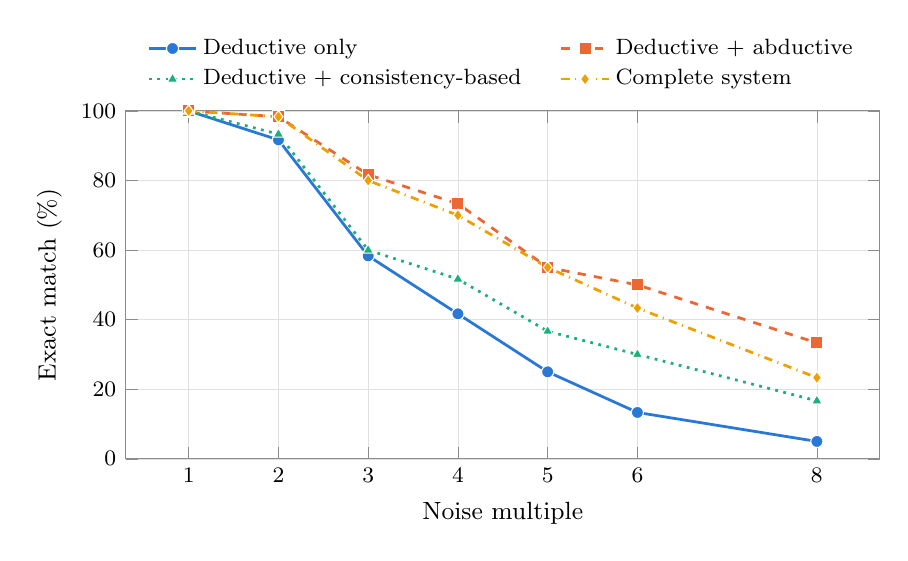
\begin{tikzpicture}
\definecolor{modedeductive}{HTML}{2a78d6}
\definecolor{modededabd}{HTML}{eb6834}
\definecolor{modededcbd}{HTML}{1baf7a}
\definecolor{modefull}{HTML}{eda100}
\begin{axis}[
  width=0.92\linewidth, height=6cm,
  xlabel={Noise multiple}, ylabel={Exact match (\%)},
  ymin=0, ymax=100,
  xtick={1,2,3,4,5,6,8},
  grid=major, major grid style={line width=0.2pt, draw=black!12},
  axis line style={draw=black!45}, tick style={draw=black!45},
  label style={font=\small}, tick label style={font=\footnotesize},
  legend style={font=\footnotesize, draw=none, fill=none, at={(0.5,1.03)}, anchor=south, legend columns=2,
    /tikz/every even column/.append style={column sep=1.2em}},
  legend cell align=left,
]
\addplot[color=modedeductive, solid, line width=1pt, mark=*, mark size=2.2pt, mark options={solid, draw=white, line width=0.4pt}] coordinates {(1,100.00) (2,91.67) (3,58.33) (4,41.67) (5,25.00) (6,13.33) (8,5.00)};
\addlegendentry{Deductive only}
\addplot[color=modededabd, dashed, line width=1pt, mark=square*, mark size=2.2pt, mark options={solid, draw=white, line width=0.4pt}] coordinates {(1,100.00) (2,98.33) (3,81.67) (4,73.33) (5,55.00) (6,50.00) (8,33.33)};
\addlegendentry{Deductive + abductive}
\addplot[color=modededcbd, dotted, line width=1pt, mark=triangle*, mark size=2.2pt, mark options={solid, draw=white, line width=0.4pt}] coordinates {(1,100.00) (2,93.33) (3,60.00) (4,51.67) (5,36.67) (6,30.00) (8,16.67)};
\addlegendentry{Deductive + consistency-based}
\addplot[color=modefull, dashdotted, line width=1pt, mark=diamond*, mark size=2.2pt, mark options={solid, draw=white, line width=0.4pt}] coordinates {(1,100.00) (2,98.33) (3,80.00) (4,70.00) (5,55.00) (6,43.33) (8,23.33)};
\addlegendentry{Complete system}
\end{axis}
\end{tikzpicture}

  \caption{Exact-match accuracy against sensor noise, by reasoning mode. Each point is 60 synthetic cases.}
  \label{fig:sens-noise}
\end{figure}

% Generated by tests/sensitivity.py. Do not edit by hand.
\begin{table}[htbp]
  \centering
  \footnotesize
  \setlength{\tabcolsep}{4pt}
  \caption{Sensitivity to sensor noise: exact match by reasoning mode, with coverage, macro F1 and mean time in milliseconds of the complete system. Each level has 60 synthetic cases. Ded.: deductive only; +Abd.: deductive and abductive; +Cons.: deductive and consistency-based; Cov.: coverage.}
  \label{tab:sens-noise}
  \begin{tabular}{lrrrrrrr}
  \toprule
  Noise multiple & Ded. & +Abd. & +Cons. & Complete & Cov. & Macro F1 & ms \\
  \midrule
  1 & 100.0\% & 100.0\% & 100.0\% & 100.0\% & 100.0\% & 1.000 & 1.36 \\
  2 & 91.7\% & 98.3\% & 93.3\% & 98.3\% & 100.0\% & 0.985 & 1.22 \\
  3 & 58.3\% & 81.7\% & 60.0\% & 80.0\% & 96.7\% & 0.894 & 1.21 \\
  4 & 41.7\% & 73.3\% & 51.7\% & 70.0\% & 95.0\% & 0.867 & 1.24 \\
  5 & 25.0\% & 55.0\% & 36.7\% & 55.0\% & 90.0\% & 0.787 & 1.42 \\
  6 & 13.3\% & 50.0\% & 30.0\% & 43.3\% & 90.0\% & 0.776 & 2.84 \\
  8 & 5.0\% & 33.3\% & 16.7\% & 23.3\% & 81.7\% & 0.693 & 5.91 \\
  \bottomrule
  \end{tabular}
\end{table}


Noise degrades deduction fastest (Figure~\ref{fig:sens-noise} and Table~\ref{tab:sens-noise}). At four times the nominal noise, deduction keeps 42\% exact match while the abductive configuration keeps 73\%. Noise is a precision problem, not a recall problem. The deductive rules still find the true fault in most noisy cases, but crisp thresholds turn noise into additional false findings. Graded evidence, scaled to the noise estimated from the case itself, and parsimony keep those findings out of the abductive explanations.

\subsection{Missing observations}

\begin{figure}[htbp]
  \centering
  % Generated by tests/sensitivity.py. Do not edit by hand.
% Needs \usepackage{pgfplots} and \pgfplotsset{compat=1.18} in the preamble.
% Colours: validated categorical palette, slots 1 to 4. Marker and dash repeat the identity.
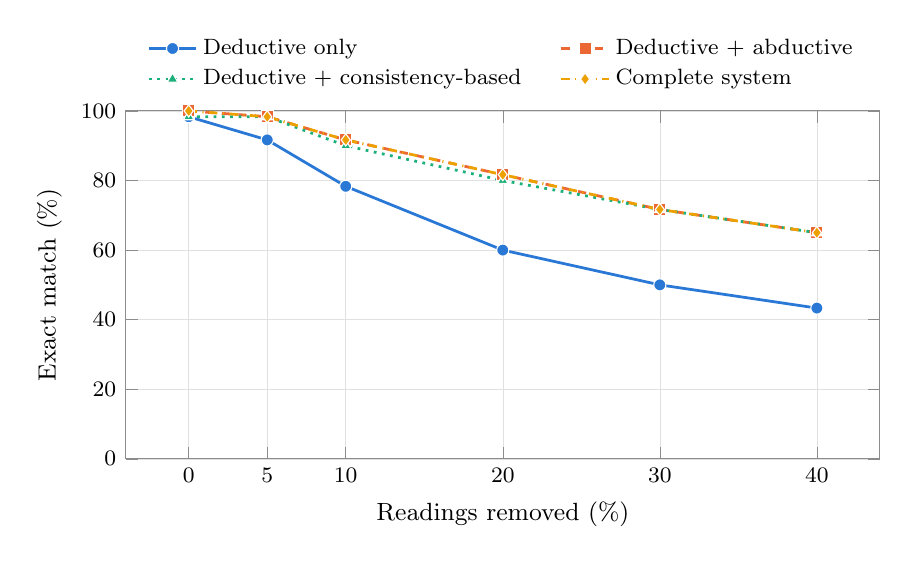
\begin{tikzpicture}
\definecolor{modedeductive}{HTML}{2a78d6}
\definecolor{modededabd}{HTML}{eb6834}
\definecolor{modededcbd}{HTML}{1baf7a}
\definecolor{modefull}{HTML}{eda100}
\begin{axis}[
  width=0.92\linewidth, height=6cm,
  xlabel={Readings removed (\%)}, ylabel={Exact match (\%)},
  ymin=0, ymax=100,
  xtick={0,5,10,20,30,40},
  grid=major, major grid style={line width=0.2pt, draw=black!12},
  axis line style={draw=black!45}, tick style={draw=black!45},
  label style={font=\small}, tick label style={font=\footnotesize},
  legend style={font=\footnotesize, draw=none, fill=none, at={(0.5,1.03)}, anchor=south, legend columns=2,
    /tikz/every even column/.append style={column sep=1.2em}},
  legend cell align=left,
]
\addplot[color=modedeductive, solid, line width=1pt, mark=*, mark size=2.2pt, mark options={solid, draw=white, line width=0.4pt}] coordinates {(0,98.33) (5,91.67) (10,78.33) (20,60.00) (30,50.00) (40,43.33)};
\addlegendentry{Deductive only}
\addplot[color=modededabd, dashed, line width=1pt, mark=square*, mark size=2.2pt, mark options={solid, draw=white, line width=0.4pt}] coordinates {(0,100.00) (5,98.33) (10,91.67) (20,81.67) (30,71.67) (40,65.00)};
\addlegendentry{Deductive + abductive}
\addplot[color=modededcbd, dotted, line width=1pt, mark=triangle*, mark size=2.2pt, mark options={solid, draw=white, line width=0.4pt}] coordinates {(0,98.33) (5,98.33) (10,90.00) (20,80.00) (30,71.67) (40,65.00)};
\addlegendentry{Deductive + consistency-based}
\addplot[color=modefull, dashdotted, line width=1pt, mark=diamond*, mark size=2.2pt, mark options={solid, draw=white, line width=0.4pt}] coordinates {(0,100.00) (5,98.33) (10,91.67) (20,81.67) (30,71.67) (40,65.00)};
\addlegendentry{Complete system}
\end{axis}
\end{tikzpicture}

  \caption{Exact-match accuracy against the share of readings removed, by reasoning mode. The three model-based configurations give almost identical results, so their lines overlap.}
  \label{fig:sens-missing}
\end{figure}

% Generated by tests/sensitivity.py. Do not edit by hand.
\begin{table}[htbp]
  \centering
  \footnotesize
  \setlength{\tabcolsep}{4pt}
  \caption{Sensitivity to missing observations: exact match by reasoning mode, with coverage, macro F1 and mean time in milliseconds of the complete system. Each level has 60 synthetic cases. Ded.: deductive only; +Abd.: deductive and abductive; +Cons.: deductive and consistency-based; Cov.: coverage.}
  \label{tab:sens-missing}
  \begin{tabular}{lrrrrrrr}
  \toprule
  Readings removed & Ded. & +Abd. & +Cons. & Complete & Cov. & Macro F1 & ms \\
  \midrule
  0\% & 98.3\% & 100.0\% & 98.3\% & 100.0\% & 100.0\% & 1.000 & 1.11 \\
  5\% & 91.7\% & 98.3\% & 98.3\% & 98.3\% & 98.3\% & 0.982 & 1.09 \\
  10\% & 78.3\% & 91.7\% & 90.0\% & 91.7\% & 91.7\% & 0.914 & 1.11 \\
  20\% & 60.0\% & 81.7\% & 80.0\% & 81.7\% & 81.7\% & 0.818 & 0.94 \\
  30\% & 50.0\% & 71.7\% & 71.7\% & 71.7\% & 71.7\% & 0.739 & 1.17 \\
  40\% & 43.3\% & 65.0\% & 65.0\% & 65.0\% & 65.0\% & 0.681 & 0.82 \\
  \bottomrule
  \end{tabular}
\end{table}


The lead of the three model-based configurations over deduction widens with the share of missing readings, from about 7 percentage points at 5\% missing to about 22 points at 20\% and beyond (Figure~\ref{fig:sens-missing}). A missing reading makes its symptom unknown rather than absent, so no hypothesis is rejected for lack of data, and a hypothesis can be accepted on its remaining evidence. A deductive rule fails as soon as one reading in its body is missing.

\subsection{Multiple simultaneous faults}

\begin{figure}[htbp]
  \centering
  % Generated by tests/sensitivity.py. Do not edit by hand.
% Needs \usepackage{pgfplots} and \pgfplotsset{compat=1.18} in the preamble.
% Colours: validated categorical palette, slots 1 to 4. Marker and dash repeat the identity.
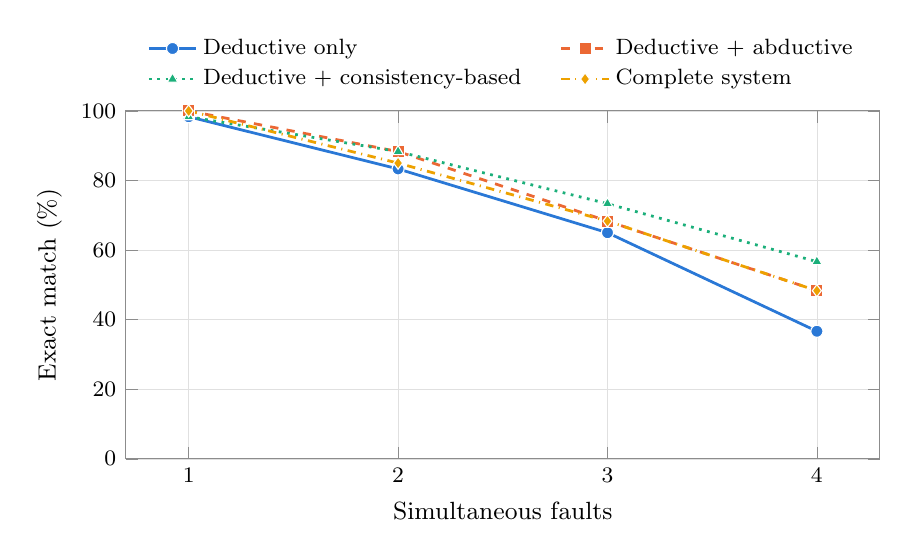
\begin{tikzpicture}
\definecolor{modedeductive}{HTML}{2a78d6}
\definecolor{modededabd}{HTML}{eb6834}
\definecolor{modededcbd}{HTML}{1baf7a}
\definecolor{modefull}{HTML}{eda100}
\begin{axis}[
  width=0.92\linewidth, height=6cm,
  xlabel={Simultaneous faults}, ylabel={Exact match (\%)},
  ymin=0, ymax=100,
  xtick={1,2,3,4},
  grid=major, major grid style={line width=0.2pt, draw=black!12},
  axis line style={draw=black!45}, tick style={draw=black!45},
  label style={font=\small}, tick label style={font=\footnotesize},
  legend style={font=\footnotesize, draw=none, fill=none, at={(0.5,1.03)}, anchor=south, legend columns=2,
    /tikz/every even column/.append style={column sep=1.2em}},
  legend cell align=left,
]
\addplot[color=modedeductive, solid, line width=1pt, mark=*, mark size=2.2pt, mark options={solid, draw=white, line width=0.4pt}] coordinates {(1,98.33) (2,83.33) (3,65.00) (4,36.67)};
\addlegendentry{Deductive only}
\addplot[color=modededabd, dashed, line width=1pt, mark=square*, mark size=2.2pt, mark options={solid, draw=white, line width=0.4pt}] coordinates {(1,100.00) (2,88.33) (3,68.33) (4,48.33)};
\addlegendentry{Deductive + abductive}
\addplot[color=modededcbd, dotted, line width=1pt, mark=triangle*, mark size=2.2pt, mark options={solid, draw=white, line width=0.4pt}] coordinates {(1,98.33) (2,88.33) (3,73.33) (4,56.67)};
\addlegendentry{Deductive + consistency-based}
\addplot[color=modefull, dashdotted, line width=1pt, mark=diamond*, mark size=2.2pt, mark options={solid, draw=white, line width=0.4pt}] coordinates {(1,100.00) (2,85.00) (3,68.33) (4,48.33)};
\addlegendentry{Complete system}
\end{axis}
\end{tikzpicture}

  \caption{Exact-match accuracy against the number of simultaneous faults, by reasoning mode.}
  \label{fig:sens-multi}
\end{figure}

% Generated by tests/sensitivity.py. Do not edit by hand.
\begin{table}[htbp]
  \centering
  \footnotesize
  \setlength{\tabcolsep}{4pt}
  \caption{Sensitivity to the number of simultaneous faults: exact match by reasoning mode, with coverage, macro F1 and mean time in milliseconds of the complete system. Each level has 60 synthetic cases. Ded.: deductive only; +Abd.: deductive and abductive; +Cons.: deductive and consistency-based; Cov.: coverage.}
  \label{tab:sens-multi}
  \begin{tabular}{lrrrrrrr}
  \toprule
  Simultaneous faults & Ded. & +Abd. & +Cons. & Complete & Cov. & Macro F1 & ms \\
  \midrule
  1 & 98.3\% & 100.0\% & 98.3\% & 100.0\% & 100.0\% & 1.000 & 1.35 \\
  2 & 83.3\% & 88.3\% & 88.3\% & 85.0\% & 93.3\% & 0.983 & 1.43 \\
  3 & 65.0\% & 68.3\% & 73.3\% & 68.3\% & 76.7\% & 0.951 & 1.40 \\
  4 & 36.7\% & 48.3\% & 56.7\% & 48.3\% & 48.3\% & 0.846 & 1.73 \\
  \bottomrule
  \end{tabular}
\end{table}


Exact-match accuracy falls as faults are combined (Figure~\ref{fig:sens-multi}). Precision stays close to 1, so the system rarely reports a fault that is not present, while recall falls as interacting faults share symptoms. Two cooling faults together, such as a fan failure and a chilled-water loss, overlap in what they show, and parsimony then prefers one fault to two. The consistency-based configuration handles four faults best, because a fault model forces it to keep a second fault whose own relation was violated. Reasoning remains fast at every fault count (Figure~\ref{fig:sens-multi-time}). The timing curves are wall-clock measurements and include some noise from other processes on the test machine, such as the dip at two faults. They should therefore be read only as an order of magnitude: a few milliseconds per case at every fault count, far below the sampling interval of data centre monitoring. Differences of a fraction of a millisecond between configurations or fault counts are not meaningful.

\begin{figure}[htbp]
  \centering
  % Generated by tests/sensitivity.py. Do not edit by hand.
% Needs \usepackage{pgfplots} and \pgfplotsset{compat=1.18} in the preamble.
% Colours: validated categorical palette, slots 1 to 4. Marker and dash repeat the identity.
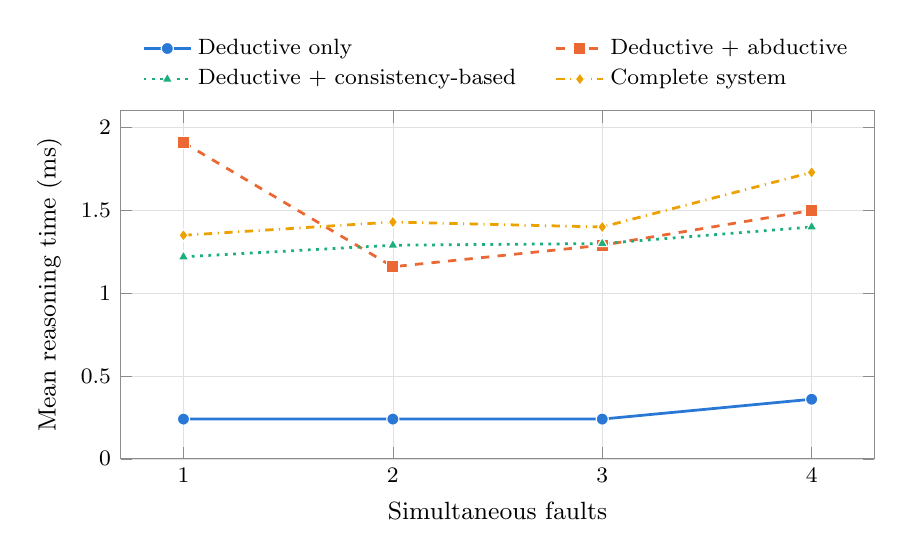
\begin{tikzpicture}
\definecolor{modedeductive}{HTML}{2a78d6}
\definecolor{modededabd}{HTML}{eb6834}
\definecolor{modededcbd}{HTML}{1baf7a}
\definecolor{modefull}{HTML}{eda100}
\begin{axis}[
  width=0.92\linewidth, height=6cm,
  xlabel={Simultaneous faults}, ylabel={Mean reasoning time (ms)},
  ymin=0,
  xtick={1,2,3,4},
  grid=major, major grid style={line width=0.2pt, draw=black!12},
  axis line style={draw=black!45}, tick style={draw=black!45},
  label style={font=\small}, tick label style={font=\footnotesize},
  legend style={font=\footnotesize, draw=none, fill=none, at={(0.5,1.03)}, anchor=south, legend columns=2,
    /tikz/every even column/.append style={column sep=1.2em}},
  legend cell align=left,
]
\addplot[color=modedeductive, solid, line width=1pt, mark=*, mark size=2.2pt, mark options={solid, draw=white, line width=0.4pt}] coordinates {(1,0.24) (2,0.24) (3,0.24) (4,0.36)};
\addlegendentry{Deductive only}
\addplot[color=modededabd, dashed, line width=1pt, mark=square*, mark size=2.2pt, mark options={solid, draw=white, line width=0.4pt}] coordinates {(1,1.91) (2,1.16) (3,1.29) (4,1.50)};
\addlegendentry{Deductive + abductive}
\addplot[color=modededcbd, dotted, line width=1pt, mark=triangle*, mark size=2.2pt, mark options={solid, draw=white, line width=0.4pt}] coordinates {(1,1.22) (2,1.29) (3,1.30) (4,1.40)};
\addlegendentry{Deductive + consistency-based}
\addplot[color=modefull, dashdotted, line width=1pt, mark=diamond*, mark size=2.2pt, mark options={solid, draw=white, line width=0.4pt}] coordinates {(1,1.35) (2,1.43) (3,1.40) (4,1.73)};
\addlegendentry{Complete system}
\end{axis}
\end{tikzpicture}

  \caption{Mean reasoning time per case against the number of simultaneous faults. Times are wall-clock and include measurement noise.}
  \label{fig:sens-multi-time}
\end{figure}

\subsection{Contradictory evidence: sensor bias}

\begin{figure}[htbp]
  \centering
  % Generated by tests/sensitivity.py. Do not edit by hand.
% Needs \usepackage{pgfplots} and \pgfplotsset{compat=1.18} in the preamble.
% Colours: validated categorical palette, slots 1 to 4. Marker and dash repeat the identity.
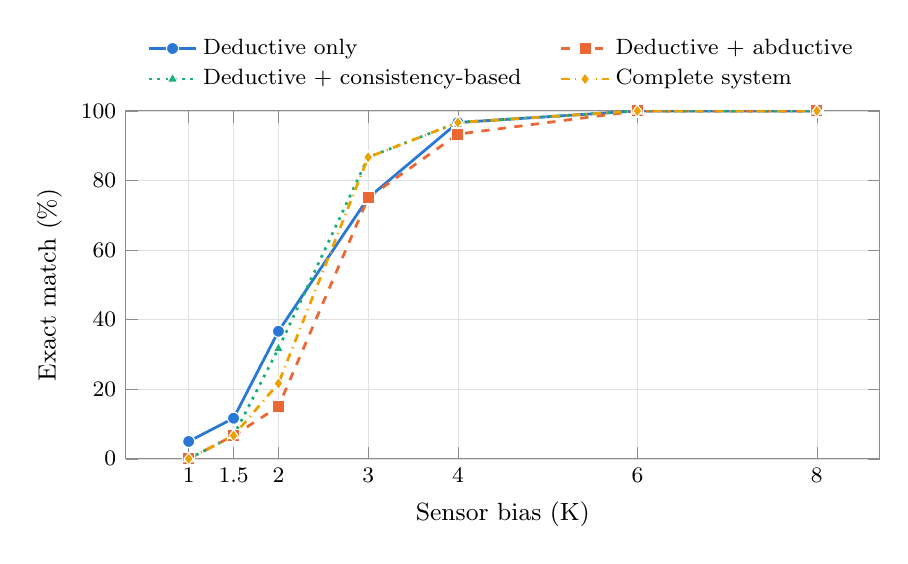
\begin{tikzpicture}
\definecolor{modedeductive}{HTML}{2a78d6}
\definecolor{modededabd}{HTML}{eb6834}
\definecolor{modededcbd}{HTML}{1baf7a}
\definecolor{modefull}{HTML}{eda100}
\begin{axis}[
  width=0.92\linewidth, height=6cm,
  xlabel={Sensor bias (K)}, ylabel={Exact match (\%)},
  ymin=0, ymax=100,
  xtick={1,1.5,2,3,4,6,8},
  grid=major, major grid style={line width=0.2pt, draw=black!12},
  axis line style={draw=black!45}, tick style={draw=black!45},
  label style={font=\small}, tick label style={font=\footnotesize},
  legend style={font=\footnotesize, draw=none, fill=none, at={(0.5,1.03)}, anchor=south, legend columns=2,
    /tikz/every even column/.append style={column sep=1.2em}},
  legend cell align=left,
]
\addplot[color=modedeductive, solid, line width=1pt, mark=*, mark size=2.2pt, mark options={solid, draw=white, line width=0.4pt}] coordinates {(1,5.00) (1.5,11.67) (2,36.67) (3,75.00) (4,96.67) (6,100.00) (8,100.00)};
\addlegendentry{Deductive only}
\addplot[color=modededabd, dashed, line width=1pt, mark=square*, mark size=2.2pt, mark options={solid, draw=white, line width=0.4pt}] coordinates {(1,0.00) (1.5,6.67) (2,15.00) (3,75.00) (4,93.33) (6,100.00) (8,100.00)};
\addlegendentry{Deductive + abductive}
\addplot[color=modededcbd, dotted, line width=1pt, mark=triangle*, mark size=2.2pt, mark options={solid, draw=white, line width=0.4pt}] coordinates {(1,0.00) (1.5,6.67) (2,31.67) (3,86.67) (4,96.67) (6,100.00) (8,100.00)};
\addlegendentry{Deductive + consistency-based}
\addplot[color=modefull, dashdotted, line width=1pt, mark=diamond*, mark size=2.2pt, mark options={solid, draw=white, line width=0.4pt}] coordinates {(1,0.00) (1.5,6.67) (2,21.67) (3,86.67) (4,96.67) (6,100.00) (8,100.00)};
\addlegendentry{Complete system}
\end{axis}
\end{tikzpicture}

  \caption{Exact-match accuracy against the size of an injected temperature-sensor bias.}
  \label{fig:sens-bias}
\end{figure}

% Generated by tests/sensitivity.py. Do not edit by hand.
\begin{table}[htbp]
  \centering
  \footnotesize
  \setlength{\tabcolsep}{4pt}
  \caption{Sensitivity to the size of a sensor bias, a source of contradictory evidence: exact match by reasoning mode, with coverage, macro F1 and mean time in milliseconds of the complete system. Each level has 60 synthetic cases. Ded.: deductive only; +Abd.: deductive and abductive; +Cons.: deductive and consistency-based; Cov.: coverage.}
  \label{tab:sens-bias}
  \begin{tabular}{lrrrrrrr}
  \toprule
  Sensor bias & Ded. & +Abd. & +Cons. & Complete & Cov. & Macro F1 & ms \\
  \midrule
  1\,K & 5.0\% & 0.0\% & 0.0\% & 0.0\% & 0.0\% & 0.000 & 0.96 \\
  1.5\,K & 11.7\% & 6.7\% & 6.7\% & 6.7\% & 6.7\% & 0.121 & 1.06 \\
  2\,K & 36.7\% & 15.0\% & 31.7\% & 21.7\% & 21.7\% & 0.317 & 1.05 \\
  3\,K & 75.0\% & 75.0\% & 86.7\% & 86.7\% & 86.7\% & 0.929 & 1.11 \\
  4\,K & 96.7\% & 93.3\% & 96.7\% & 96.7\% & 96.7\% & 0.983 & 1.13 \\
  6\,K & 100.0\% & 100.0\% & 100.0\% & 100.0\% & 100.0\% & 1.000 & 1.18 \\
  8\,K & 100.0\% & 100.0\% & 100.0\% & 100.0\% & 100.0\% & 1.000 & 1.63 \\
  \bottomrule
  \end{tabular}
\end{table}


A biased sensor contradicts its neighbours and the energy balances. Biases below the 2\,K neighbour-deviation threshold are rarely detected, which is the expected limit of the design, and biases of 4\,K or more are detected almost always (Figure~\ref{fig:sens-bias}). At 3\,K the consistency-based configurations do best, because a single sensor fault is then the only minimal diagnosis that removes every conflict. At 2\,K the graded modes are deliberately more cautious than deduction, because they require one noise standard deviation of margin past the threshold.

\subsection{Threshold changes}

Each threshold was perturbed on its own on the held-out split (Table~\ref{tab:sens-thresholds}). Eleven of the 23 thresholds change nothing at any level, because backup rules or other symptoms cover them, or because no case lies near them. At $\pm$1\,K or $\pm$10\%, all but three change the complete system's accuracy by less than 3 percentage points.

% Generated by tests/sensitivity.py from docs/10b_threshold_sensitivity.md. Do not edit by hand.
\begin{footnotesize}
\setlength{\tabcolsep}{4pt}
\begin{longtable}{L{4.4cm}L{1.6cm}rrrrr}
  \caption{Threshold sensitivity on the held-out split: change in exact-match accuracy of the complete system, in percentage points, when one threshold is perturbed. Temperature thresholds move by $-2$, $-1$, $+1$ and $+2$\,K; other thresholds are scaled by 0.8, 0.9, 1.1 and 1.2. The last column is the worst change for deduction alone. A dot means no change.}\label{tab:sens-thresholds}\\
  \toprule
  Threshold & Base & $-2$ / 0.8 & $-1$ / 0.9 & $+1$ / 1.1 & $+2$ / 1.2 & Ded. worst \\
  \midrule
  \endfirsthead
  \toprule
  Threshold & Base & $-2$ / 0.8 & $-1$ / 0.9 & $+1$ / 1.1 & $+2$ / 1.2 & Ded. worst \\
  \midrule
  \endhead
  \texttt{t\_\allowbreak{}inlet\_\allowbreak{}rec\_\allowbreak{}max} & 27.0 \textdegree C & $\cdot$ & $\cdot$ & $\cdot$ & $\cdot$ & $\cdot$ \\
  \texttt{t\_\allowbreak{}inlet\_\allowbreak{}rec\_\allowbreak{}min} & 18.0 \textdegree C & $\cdot$ & $\cdot$ & $\cdot$ & $\cdot$ & $\cdot$ \\
  \texttt{t\_\allowbreak{}supply\_\allowbreak{}band} & 2.0 K & $\cdot$ & $\cdot$ & $\cdot$ & $\cdot$ & -7.5 \\
  \texttt{row\_\allowbreak{}hot\_\allowbreak{}fraction} & 0.5 & $\cdot$ & $\cdot$ & $\cdot$ & $\cdot$ & $\cdot$ \\
  \texttt{valve\_\allowbreak{}open\_\allowbreak{}min} & 50.0 \% & $\cdot$ & $\cdot$ & $\cdot$ & $\cdot$ & $\cdot$ \\
  \texttt{chw\_\allowbreak{}flow\_\allowbreak{}ratio\_\allowbreak{}min} & 0.3 & -0.8 & -0.8 & $\cdot$ & $\cdot$ & $\cdot$ \\
  \texttt{strat\_\allowbreak{}max} & 3.0 K & -77.3 & -2.7 & $\cdot$ & -0.8 & -90.2 \\
  \texttt{fan\_\allowbreak{}ratio\_\allowbreak{}min} & 0.5 & $\cdot$ & $\cdot$ & $\cdot$ & $\cdot$ & $\cdot$ \\
  \texttt{strat\_\allowbreak{}out\_\allowbreak{}max} & 3.5 K & -50.2 & -1.2 & -4.3 & -8.2 & -76.5 \\
  \texttt{filter\_\allowbreak{}loading\_\allowbreak{}max} & 1.7 & 0.8 & $\cdot$ & -0.8 & -2.0 & -1.2 \\
  \texttt{server\_\allowbreak{}fan\_\allowbreak{}min} & 1000.0 rpm & $\cdot$ & $\cdot$ & $\cdot$ & $\cdot$ & $\cdot$ \\
  \texttt{cpu\_\allowbreak{}hot\_\allowbreak{}min} & 85.0 \textdegree C & $\cdot$ & $\cdot$ & $\cdot$ & $\cdot$ & $\cdot$ \\
  \texttt{branch\_\allowbreak{}loading\_\allowbreak{}max} & 0.8 & 0.8 & 0.8 & -3.9 & -9.0 & -9.0 \\
  \texttt{cell\_\allowbreak{}r\_\allowbreak{}ratio\_\allowbreak{}max} & 1.3 & -30.2 & 0.8 & -0.4 & -0.8 & -43.9 \\
  \texttt{ups\_\allowbreak{}eff\_\allowbreak{}bypass\_\allowbreak{}min} & 0.98 & -84.3 & -83.9 & $\cdot$ & $\cdot$ & -1.2 \\
  \texttt{neighbour\_\allowbreak{}dev\_\allowbreak{}max} & 2.0 K & -85.1 & -0.4 & $\cdot$ & $\cdot$ & -87.8 \\
  \texttt{balance\_\allowbreak{}resid\_\allowbreak{}max} & 0.2 & $\cdot$ & $\cdot$ & $\cdot$ & $\cdot$ & $\cdot$ \\
  \texttt{sample\_\allowbreak{}age\_\allowbreak{}max} & 60.0 s & $\cdot$ & $\cdot$ & $\cdot$ & $\cdot$ & $\cdot$ \\
  \texttt{t\_\allowbreak{}supply\_\allowbreak{}hot\_\allowbreak{}limit} & 22.0 \textdegree C & -12.5 & $\cdot$ & $\cdot$ & $\cdot$ & $\cdot$ \\
  \texttt{fan\_\allowbreak{}ratio\_\allowbreak{}reduced} & 0.85 & $\cdot$ & $\cdot$ & $\cdot$ & -45.5 & -7.1 \\
  \texttt{t\_\allowbreak{}supply\_\allowbreak{}cold\_\allowbreak{}limit} & 18.0 \textdegree C & $\cdot$ & $\cdot$ & $\cdot$ & -11.4 & $\cdot$ \\
  \texttt{power\_\allowbreak{}resid\_\allowbreak{}max} & 0.1 & -0.4 & $\cdot$ & 0.4 & 0.4 & $\cdot$ \\
  \texttt{sensor\_\allowbreak{}noise\_\allowbreak{}floor} & 0.15 K & $\cdot$ & $\cdot$ & $\cdot$ & $\cdot$ & $\cdot$ \\
  \bottomrule
\end{longtable}
\end{footnotesize}


The large drops share one cause: each occurs when the perturbed threshold moves inside the scatter of normal operation. Moving the inlet stratification limit to 1\,K, inside the 1 to 2.2\,K of sealed racks, costs 77 points. Scaling the reduced-fan-power limit to 1.02, inside the $\pm$5\% scatter of a healthy fan, costs 46 points. This is evidence that each threshold sits in a margin between the normal envelope and the fault envelope, and the table measures how wide each margin is.

One result is a warning about consistency checking. Scaling the UPS-efficiency threshold to 0.88 puts every healthy double-conversion UPS, which runs near 0.955, above it. Deduction loses only 1.2 points, because its UPS rule relies on the mode flag. The complete system loses 84 points, because the mis-set relation produces a conflict in every case and the consistency module then rejects every correct explanation. A redundancy relation acts as a hard constraint, so a wrong relation threshold corrupts every diagnosis. Relation thresholds should therefore be derived from sensor uncertainty (Equation~\eqref{eq:uncertainty}) and validated on normal data before deployment.

\subsection{Reasoning parameters}
\label{sec:param-sensitivity}

The threshold study does not cover the five reasoning parameters set by judgement (Table~\ref{tab:design-params}). Each was changed on its own, and the three model-based configurations were run on both splits and on four stress sets from this section: four times the nominal noise, 20\% of readings missing, four simultaneous faults, and a 2\,K sensor bias, which lies in the transition between missed and detected biases. Table~\ref{tab:param-sensitivity} gives the results. Deduction uses none of these parameters and is the reference. The study is generated by \texttt{tests/param\_sensitivity.py}.

% Generated by tests/param_sensitivity.py. Do not edit by hand.
\begin{table}[htbp]
  \centering
  \scriptsize
  \setlength{\tabcolsep}{3pt}
  \caption{Sensitivity to the reasoning parameters set by judgement. Each parameter is changed alone. The first two rows give exactly matched cases at the defaults; the other rows give the change in exactly matched cases, for deductive + abductive / deductive + consistency-based / complete system. For the perturbed weights, the range over five random draws is given in brackets. Defaults: bonus 0.1, cut-off $k = 1$, search bound 4, weights from \texttt{kb/causal.pl}, noise of unredundant features tied to $\sigma_T$. Raw counts are in \texttt{docs/15\_parameter\_sensitivity.md}.}
  \label{tab:param-sensitivity}
  \begin{tabular}{L{2.3cm}lcccccc}
  \toprule
  Parameter & Value & Calibration & Held-out & Noise $\times$4 & 20\% missing & Four faults & 2 K bias \\
  \midrule
  Deduction only & & 230 & 232 & 25 & 36 & 22 & 22 \\
  Model-based & default & 238/234/238 & 241/238/239 & 44/31/42 & 49/48/49 & 29/34/29 & 9/19/13 \\
  \midrule
  Deductive bonus & 0 & 0/0/0 & 0/0/0 & 0/0/0 & 0/0/0 & 0/0/0 & 0/0/0 \\
   & 0.05 & 0/0/0 & 0/0/0 & 0/0/0 & 0/0/0 & 0/0/0 & 0/0/0 \\
   & 0.2 & 0/0/0 & +1/0/+1 & +1/0/+1 & 0/0/0 & 0/0/0 & 0/0/0 \\
   & 0.5 & 0/0/0 & +2/0/+2 & +1/0/+1 & 0/0/0 & 0/0/0 & +6/0/+6 \\
  \addlinespace
  Cut-off $k$ & 0.5 & $-$3/$-$1/$-$2 & $-$3/$-$4/$-$4 & $-$7/$-$7/$-$9 & 0/0/0 & 0/0/0 & +6/+4/+9 \\
   & 1.5 & 0/+1/0 & +1/$-$1/+1 & +2/+4/+4 & 0/0/0 & 0/0/0 & $-$2/$-$2/$-$3 \\
   & 2.0 & +1/+1/+1 & +1/+2/+2 & +3/+6/+5 & 0/0/0 & 0/0/0 & $-$2/$-$4/$-$5 \\
  \addlinespace
  Search bound & 2 & 0/0/0 & 0/+1/0 & +1/+1/0 & 0/0/0 & $-$29/$-$12/$-$29 & 0/0/0 \\
   & 3 & 0/0/0 & 0/0/0 & +1/0/0 & 0/0/0 & $-$29/$-$12/$-$29 & 0/0/0 \\
   & 5 & 0/0/0 & 0/0/0 & 0/0/0 & 0/0/0 & 0/$-$4/0 & 0/0/0 \\
  \addlinespace
  Causal weights & all 1 & 0/0/0 & 0/0/0 & 0/0/0 & $-$1/0/$-$1 & 0/0/0 & 0/0/0 \\
   & $\times$U[.5,1.5] & $-$1/0/$-$1 & 0/0/0 & 0/0/0 & [0,+1]/0/[0,+1] & 0/0/0 & 0/0/0 \\
  \addlinespace
  Noise scaling & fixed & +1/+1/+1 & 0/0/0 & $-$1/$-$3/$-$4 & 0/0/0 & 0/0/0 & 0/0/0 \\
  \bottomrule
  \end{tabular}
\end{table}


\begin{itemize}
  \item \textbf{Causal weights hardly matter.} Setting every weight to 1, or multiplying each by a random factor between 0.5 and 1.5 in five independent draws, changes at most one case on any set. Parsimony, not the weights, decides most explanations, and the weights only rank explanations of the same size.
  \item \textbf{The deductive bonus hardly matters up to 0.2.} At 0.5 it gains two held-out cases and six 2\,K-bias cases, because abduction then defers to the rules, which detect small biases better (Section~\ref{sec:sensitivity}). It leaves the calibration split unchanged.
  \item \textbf{The evidence cut-off is a real trade-off.} A looser cut-off, $k = 0.5$, catches four to nine more 2\,K biases but loses seven to nine cases under heavy noise. A stricter one, $k = 2$, gains three to six noisy cases and loses two to five small biases. The default $k = 1$ lies between them: on the held-out split it is at most two cases behind the stricter cut-off and three or four ahead of the looser one.
  \item \textbf{The search bound must cover the largest fault combination.} A bound of 2 or 3 loses every four-fault case of the abductive configurations, and 12 of the consistency-based one. A bound of 5 changes nothing, except that consistency-based search then accepts larger, wrong diagnoses in four of the four-fault cases.
  \item \textbf{Tying the noise of unredundant features to the temperature sensors helps under noise.} With fixed nominal noise instead, the model-based configurations lose one to four cases at four times the noise, and gain one calibration case.
\end{itemize}

The defaults were set before this study and were not changed after it. The held-out split must not be used to tune them, and on the calibration split no variant except the search bound and the loosest cut-off moves any configuration by more than one case, so the calibration data give no reason to change them either. The results support the claim that the conclusions of this chapter do not depend on the exact values chosen by judgement, except for the evidence cut-off, which sets the balance between robustness to noise and sensitivity to small faults.

\subsection{Summary}

Table~\ref{tab:sens-summary} summarises the findings of the sensitivity and ablation analysis.

\begin{table}[htbp]
  \centering
  \small
  \caption{Summary of the sensitivity analysis.}
  \label{tab:sens-summary}
  \begin{tabular}{L{4.2cm}L{9.8cm}}
    \toprule
    Question & Finding \\
    \midrule
    Threshold changes & Robust within $\pm$1\,K or $\pm$10\%. Large losses only when a threshold enters normal scatter. Consistency checking is sensitive to wrong relation thresholds. \\
    Missing observations & The model-based configurations lead deduction by about 7 points at 5\% missing, widening to about 22 points at 20\% and beyond. \\
    Contradictory evidence & Sensor biases of 3\,K and more are reliably found; consistency checking is best at the detection limit. \\
    Noisy data & Abduction with noise-adaptive evidence is the most robust configuration. \\
    Multiple faults & Precision stays near 1; recall falls with the number of faults because interacting faults share symptoms. \\
    Reasoning parameters & Causal weights and the deductive bonus hardly matter. The evidence cut-off trades robustness to noise against sensitivity to small faults. The search bound must cover the largest fault combination. \\
    Reasoning time & A few milliseconds per case in every sweep. \\
    \bottomrule
  \end{tabular}
\end{table}

% ---------------------------------------------------------------------------
\section{Robustness to Model Mismatch}
\label{sec:mismatch}

Every result so far was obtained on cases generated by the same engineering model that the knowledge base encodes. This section asks how much the diagnosis depends on that model being exactly right.

\paragraph{Method.} The 255 held-out cases were regenerated with the same seed, and so with the same faults, severities and random draws, but with deliberately changed simulator physics. Table~\ref{tab:mismatch-profiles} lists the two profiles. They change the coil heat transfer, server power and airflow, CPU thermal behaviour, the share of airflow shortfall drawn from the hot aisle, natural recirculation, room temperature, fan-control margin and sensor noise. Equipment ratings that a real knowledge base would take from nameplates, such as the fan's rated power and the valve characteristic, were left unchanged. The knowledge base was not modified. Because each case keeps its faults and draws, the results are compared with the nominal split case by case.

\begin{table}[htbp]
  \centering
  \small
  \caption{Simulator physics in the two model-mismatch profiles.}
  \label{tab:mismatch-profiles}
  \begin{tabular}{L{6.8cm}rrr}
    \toprule
    Parameter & Nominal & Mild & Strong \\
    \midrule
    Coil air-side conductance (kW/K) & 15 & 12 & 10 \\
    Coil water-side conductance at design flow (kW/K) & 10 & 12 & 14 \\
    Server idle and full-load power (kW) & 0.40, 0.90 & 0.35, 0.95 & 0.30, 1.05 \\
    Server airflow at nominal fan speed (kg/s) & 0.055 & 0.050 & 0.045 \\
    CPU share of server power & 0.55 & 0.50 & 0.60 \\
    CPU thermal resistance (K/kW) & 90 & 90 & 110 \\
    Share of airflow shortfall from the hot aisle & 0.4 & 0.5 & 0.6 \\
    Natural recirculation at the top of a sealed rack & 0.10 & 0.12 & 0.15 \\
    Fan-control airflow margin & 1.10 & 1.15 & 1.25 \\
    Room air temperature (\textdegree C) & 25 & 26 & 27 \\
    Sensor noise, multiple of nominal & 1.0 & 1.25 & 1.5 \\
    \bottomrule
  \end{tabular}
\end{table}

% Generated by tests/mismatch.py. Do not edit by hand.
\begin{table}[htbp]
  \centering
  \footnotesize
  \setlength{\tabcolsep}{4pt}
  \caption{Model mismatch: exact match of each reasoning mode when the held-out cases are regenerated with changed simulator physics and diagnosed with the unchanged knowledge base. The last pair of columns re-baselines three envelope thresholds from normal operating data only. $p$: exact McNemar test against the nominal split, paired case by case. Confidence intervals are in \texttt{docs/12\_model\_mismatch.md}.}
  \label{tab:mismatch}
  \begin{tabular}{L{3.2cm}rrrrrrr}
  \toprule
  Mode & Nominal & Mild & $p$ & Strong & $p$ & Re-baselined & $p$ \\
  \midrule
  Deductive only & 91.0\% & 80.8\% & \textbf{\textless\,0.001} & 26.3\% & \textbf{\textless\,0.001} & 75.3\% & \textbf{\textless\,0.001} \\
  Deductive + abductive & 94.5\% & 91.0\% & \textbf{0.004} & 40.0\% & \textbf{\textless\,0.001} & 83.1\% & \textbf{\textless\,0.001} \\
  Deductive + consistency-based & 93.3\% & 86.3\% & \textbf{\textless\,0.001} & 33.7\% & \textbf{\textless\,0.001} & 83.5\% & \textbf{\textless\,0.001} \\
  Complete system & 93.7\% & 90.2\% & \textbf{0.004} & 39.6\% & \textbf{\textless\,0.001} & 82.4\% & \textbf{\textless\,0.001} \\
  \bottomrule
  \end{tabular}
\end{table}

% Generated by tests/mismatch.py. Do not edit by hand.
\begin{table}[htbp]
  \centering
  \small
  \caption{Model mismatch by test category: exact matches of the complete system.}
  \label{tab:mismatch-categories}
  \begin{tabular}{L{3.4cm}rrrrr}
  \toprule
  Category & Cases & Nominal & Mild & Strong & Re-baselined \\
  \midrule
  Normal & 30 & 30 & 30 & 13 & 30 \\
  Single faults & 120 & 120 & 117 & 57 & 111 \\
  Instrumentation & 30 & 30 & 29 & 6 & 29 \\
  Multiple faults & 30 & 29 & 28 & 14 & 17 \\
  Incomplete & 15 & 14 & 13 & 5 & 13 \\
  High noise & 15 & 7 & 4 & 1 & 3 \\
  Borderline & 15 & 9 & 9 & 5 & 7 \\
  \bottomrule
  \end{tabular}
\end{table}


\paragraph{Mild mismatch.} With the physics changed by about 10 to 25\%, the configurations with abduction lose about four points of exact-match accuracy, keeping 90 to 91\%, while deduction alone falls from 91.0\% to 80.8\% (Table~\ref{tab:mismatch}). Every configuration loses significantly, but graded, noise-adaptive evidence makes the model-based configurations markedly less sensitive to model error than crisp rules.

\paragraph{Strong mismatch.} With changes of about 25 to 50\%, every configuration collapses, to between 26\% and 40\%. Even 17 of the 30 normal cases are misdiagnosed (Table~\ref{tab:mismatch-categories}). Inspection of the failures shows that the reasoning is intact and that three envelope thresholds are to blame. With less airflow per server and more natural recirculation, healthy racks stratify by 3 to 4\,K, above the 3\,K and 3.5\,K stratification thresholds. With hotter-running CPUs, healthy servers exceed the 85\,\textdegree C CPU threshold. The system then sees recirculation where there is none, or symptoms that no hypothesis explains. The thresholds encode the normal envelope of the nominal model, and the strong profile moves that envelope.

\paragraph{Re-baselining from normal operating data.} A real site has plenty of data from normal operation, even when it has no fault data. To test whether that is enough, normal-only cases were generated under the strong physics with a different seed (20261020). Each of the three envelope thresholds was shifted by how far the largest normal value moved, which keeps its original margin above normal operation. No fault labels were used. The shifts were $+2.3$\,K and $+2.2$\,K for the inlet and outlet stratification thresholds and $+26.7$\,K for the CPU threshold. Re-baselining restores the complete system to 82.4\% and the other model-based configurations to about 83\%, against 75.3\% for deduction. Normal and instrumentation cases are again almost all correct. Multiple faults, at 17 of 30, and high-noise cases recover only partly. The re-baselined CPU threshold also lies above the throttling limit, so CPU temperature no longer helps to detect a failed server fan.

\paragraph{Implication.} The diagnostic reasoning transfers across models, but fixed absolute thresholds do not. A deployment would therefore need its envelope thresholds calibrated against the site's own normal operation before use. Defining those thresholds relative to a learned baseline, rather than as fixed values, is the most direct improvement this experiment suggests (Section~\ref{sec:future}).

% ---------------------------------------------------------------------------
\section{Comparison with a Data-Driven Baseline}
\label{sec:baseline}

Fault diagnosis in data centres has mostly been data-driven (Chapter~\ref{ch:theory_and_kr}), and this project offers explainability instead. That trade-off should be shown, not asserted. Standard classifiers were therefore trained on the raw readings, with no engineering knowledge, and tested on the same cases as the expert system. The framework forbids replacing the symbolic system with machine learning, not comparing against it, so the classifiers are a baseline only and play no part in the expert system.

\paragraph{Method.} Each case becomes one vector of every reading, with a missing reading left missing. The labels are the fault labels seen in training, such as chw\_supply\_loss(crah\_1), learned as one binary output each. A case with no predicted fault is predicted normal. A random forest of 300 trees and a single decision tree were trained with the standard settings of scikit-learn \parencite{pedregosa2011}, without tuning, in two regimes: on the calibration split, the 255 cases against which the knowledge base was checked, and on 2550 further simulated cases, far more labelled fault data than a real site would have. The second regime favours the classifiers in two ways: they see labelled examples of nearly every fault at every location, and they are trained and tested on the same simulator. The script is \texttt{tests/baseline.py}.

% Generated by tests/baseline.py. Do not edit by hand.
\begin{table}[htbp]
  \centering
  \footnotesize
  \setlength{\tabcolsep}{4pt}
  \caption{Exact match of the expert system and of data-driven classifiers trained on the raw readings, on the same test cases (255 held-out, 1275 over five seeds, 255 per mismatch profile). The classifiers are a baseline for comparison only. Bold: significantly different from deductive + abductive reasoning on the same cases (exact McNemar, $p < 0.05$). Details in \texttt{docs/17\_baseline\_comparison.md}.}
  \label{tab:baseline}
  \begin{tabular}{L{3.5cm}L{3.0cm}rrrr}
  \toprule
  System & Training data & Held-out & Five seeds & Mild mismatch & Strong mismatch \\
  \midrule
  Deductive + abductive & none & 94.5 & 93.6 & 91.0 & 40.0 \\
  Complete system & none & 93.7 & 92.9 & 90.2 & 39.6 \\
  \midrule
  Random forest & calibration (255) & \textbf{53.3} & \textbf{52.1} & \textbf{34.9} & \textbf{23.9} \\
  Decision tree & calibration (255) & \textbf{53.7} & \textbf{57.9} & \textbf{38.0} & \textbf{29.0} \\
  Random forest & 2550 extra cases & \textbf{82.0} & \textbf{82.0} & \textbf{48.6} & \textbf{30.6} \\
  Decision tree & 2550 extra cases & \textbf{89.4} & \textbf{87.1} & \textbf{50.2} & 38.0 \\
  \bottomrule
  \end{tabular}
\end{table}


Table~\ref{tab:baseline} gives the results. Four findings stand out.

\begin{itemize}
  \item \textbf{With the data the knowledge base was checked against, the classifiers fail.} Trained on the 255 calibration cases, they reach 52 to 58\% exact match. A fault label names its location, so there are dozens of labels with a few examples each, and 23 held-out cases contain a label never seen in training. No instrumentation case and only 2 of the 30 multiple-fault cases are diagnosed correctly.
  \item \textbf{With ten times as much labelled data, they come closer but stay significantly behind.} Trained on 2550 cases, the decision tree reaches 89.4\% on the held-out split and 87.1\% over five seeds, against 94.5\% and 93.6\% for deductive + abductive reasoning. The random forest, at 82.0\%, does worse than the single tree with these untuned settings. The classifiers do better than the expert system on borderline and high-noise cases: the forest gets 12 and 13 of 15 right against 9 and 9. Boundaries learned from labelled data fit the simulator's noise better than thresholds set by engineering judgement, and that is the price of sourced, explainable thresholds.
  \item \textbf{Under model mismatch, the classifiers collapse first.} With the physics changed by 10 to 25\%, the classifiers trained on 2550 cases fall to about 50\%, while deductive + abductive reasoning keeps 91.0\%. The classifiers have learned the exact envelope of the nominal simulator, not the physics behind it. Under strong mismatch every system fails, and the best classifier, at 38.0\%, is not significantly different from the expert system, at 40.0\%.
  \item \textbf{The classifiers explain nothing.} They give no proof, no competing hypotheses and no maintenance plan, they need labelled examples of every fault at every location, and they cannot diagnose a fault at a location absent from their training data.
\end{itemize}

On these data, then, the knowledge-based system is more accurate than standard classifiers, needs no labelled fault data, and transfers far better to a changed model, while also explaining every diagnosis. The classifiers' advantage on borderline and noisy cases is the strongest argument for learning thresholds from data within the symbolic system, as Section~\ref{sec:future} proposes, rather than for replacing it.


\chapter{Expert-System Software Development, Documentation and Reproducibility}
\label{ch:software_and_reproducibility}

Source code alone does not show how a system was built or whether its results can be trusted. This chapter documents the development lifecycle (Section~\ref{sec:process}), the implementation environment (Section~\ref{sec:environment}), the software structure and its design decisions (Section~\ref{sec:structure}), the main problems found and fixed during debugging (Section~\ref{sec:debugging}), how the software was verified and validated (Section~\ref{sec:vandv}), and exactly how to run it and reproduce every result (Sections~\ref{sec:execution} and~\ref{sec:reproducibility}).

% ---------------------------------------------------------------------------
\section{Development Process}
\label{sec:process}

Development followed the lifecycle that the project framework prescribes:
\begin{center}
  Requirements $\rightarrow$ Knowledge acquisition $\rightarrow$ Predicate design $\rightarrow$ Rule design $\rightarrow$\\
  Implementation $\rightarrow$ Debugging $\rightarrow$ Testing $\rightarrow$ Validation.
\end{center}
In practice the later stages fed back into the earlier ones. Table~\ref{tab:lifecycle} summarises what each stage produced. The design documents in the \texttt{docs/} folder record each stage as it was carried out, and much of Chapters~\ref{ch:theory_and_kr} to~\ref{ch:dataset_and_evaluation} is drawn from them.

\begin{table}[htbp]
  \centering
  \small
  \caption{Development lifecycle and its products.}
  \label{tab:lifecycle}
  \begin{tabular}{L{3.0cm}L{6.4cm}L{4.6cm}}
    \toprule
    Stage & Work done & Product \\
    \midrule
    Requirements & System boundary, fault universe, observation vector, test categories & \texttt{docs/01} to \texttt{docs/03} \\
    Knowledge acquisition & Standards, literature and engineering assumptions, each with provenance & \texttt{docs/04}, \texttt{kb/sources.pl} \\
    Predicate design & Representation of facts, observations, thresholds and calculations & \texttt{kb/components.pl}, \texttt{kb/calculations.pl} \\
    Rule design & Deductive rules, causal signatures, redundancy relations and fault models & \texttt{kb/rules.pl}, \texttt{kb/causal.pl}, \texttt{kb/arr.pl} \\
    Implementation & Meta-interpreter, abductive and consistency-based engines, explanation facility & \texttt{engine/} \\
    Testing & Physics simulator, calibration and held-out splits, sensitivity sweeps & \texttt{simulator/}, \texttt{tests/} \\
    Validation & Generalisation to the held-out split; explanation inspection; sensitivity analysis & Chapter~\ref{ch:dataset_and_evaluation} \\
    \bottomrule
  \end{tabular}
\end{table}

The system grew incrementally. A first prototype covered three faults and normal operation, end to end from readings to explanation and maintenance plan. The simulator was built next, so that every later rule could be tested against physically consistent data before it was accepted. Rules for the remaining faults followed. The abductive and consistency-based modules were added last, once the deductive layer was stable, and were evaluated against it.

% ---------------------------------------------------------------------------
\section{Implementation Environment}
\label{sec:environment}

Table~\ref{tab:environment} lists the software used. The expert system needs only SWI-Prolog. Python, with its standard library alone, generates the synthetic data and formats results. LaTeX is needed only to build this report.

\begin{table}[htbp]
  \centering
  \small
  \caption{Implementation environment.}
  \label{tab:environment}
  \begin{tabular}{L{3.6cm}L{4.0cm}L{6.4cm}}
    \toprule
    Component & Version & Role \\
    \midrule
    Operating system & Windows 11 Pro, build 26200 & Development and testing \\
    SWI-Prolog & 10.0.2, 64-bit & All diagnostic reasoning; no extra packages \\
    Python & 3.13.1, standard library only & Simulator, sensitivity driver, reproduction check \\
    scikit-learn & 1.9.1, with NumPy 2.5.4; optional & Data-driven baseline only (Section~\ref{sec:baseline}) \\
    MiKTeX & 25.12, pdfTeX 4.23 & Building the report \\
    Biber & 2.21 & Bibliography processing \\
    Strawberry Perl & 5.42.3 & Needed by the MiKTeX tool chain \\
    \bottomrule
  \end{tabular}
\end{table}

The Prolog code uses only standard built-ins and the SWI-Prolog libraries that load automatically, such as \texttt{lists}, \texttt{apply}, \texttt{yall} and \texttt{solution\_sequences}. It should run unchanged on Linux and macOS, although it has been tested only on Windows.

% ---------------------------------------------------------------------------
\section{Software Structure}
\label{sec:structure}

The source modules are listed in Table~\ref{tab:modules} and their main predicates in Table~\ref{tab:predicates}. The framework asks how several design questions were answered. Each is summarised below, with a pointer to the fuller treatment.

\paragraph{Why each major predicate exists.} Each predicate implements one component of the architecture in Figure~\ref{fig:architecture}. Calculation predicates implement single equations and carry their equation tags. \texttt{prove/2} exists so that rules can be stored as data and still yield proof trees. \texttt{case\_symptoms/2} exists so that the abductive and consistency-based modules see identical, cached evidence. \texttt{diagnose\_mode/3} exists so that the four configurations can be compared on the same data.

\paragraph{How facts are represented.} Structure, ratings, thresholds and sources are ground facts. Each test case is a separate set of \texttt{obs/4} facts, so the same knowledge base diagnoses every case unchanged (Section~\ref{sec:kb-design}).

\paragraph{How rules were constructed.} Every rule began as a row of the fault taxonomy or a physical relation from Section~\ref{sec:maths}. It was written as a Horn clause over named thresholds, given an identifier and a source, and accepted only after it had been run against the calibration split (Section~\ref{sec:predicates}).

\paragraph{How conflicts are handled.} Conflicting conclusions are resolved at four levels:
\begin{itemize}
  \item When several rules prove the same fault, it is reported once, with the first proof.
  \item Rules that could fire on a confounder are guarded by negation as failure. The recirculation rule r22, for example, is blocked if the top inlet sensor can be shown to be suspect.
  \item Competing hypotheses are resolved by abduction, through parsimony and confidence ranking (Section~\ref{sec:abductive}).
  \item Explanations that contradict a redundancy relation or a fault model are rejected by the consistency check (Section~\ref{sec:cbd}).
\end{itemize}
When two diagnoses call for maintenance plans that depend on each other, the plan interactions order the work (Section~\ref{sec:planner}).

\paragraph{How explanations are generated.} The explanation facility reads the proof trees of the deductive rules and the evidence records of the abductive and consistency-based modules. It never reconstructs reasoning after the fact (Section~\ref{sec:explanation}).

\paragraph{How maintenance actions are encoded.} Each fault class has one \texttt{maintenance/5} fact, with priority, ordered actions, rationale and source, instantiated for the diagnosed entity (Section~\ref{sec:planner}).

\paragraph{Generated documentation.} Four kinds of documentation are generated from the code and data rather than written by hand, so they cannot drift from the implementation: the rule, threshold and provenance tables (\texttt{tests/export\_latex.pl}), the evaluation tables (\texttt{tests/metrics\_latex.pl}), the sensitivity tables and figures (\texttt{tests/sensitivity.py}), and the explanation listing, which is unedited program output.

% ---------------------------------------------------------------------------
\section{Debugging}
\label{sec:debugging}

The most instructive problems found during development fall into three groups.

\subsection{Knowledge errors found by the simulator}

Because the simulator injects faults into the physics rather than the readings, it revealed errors in the knowledge itself that hand-made test cases had not. The three most significant are described in Section~\ref{sec:acquisition}: a wrong signature for chilled-water loss, a power design that made overload rules fire on healthy racks, and a stratification rule broken by server fan control. Three further problems were found the same way:

\begin{itemize}
  \item \textbf{Partial fan failures were missed.} A slipping belt that leaves the fan drawing 55\% of its expected power passed the 0.5 threshold for a failed fan, so the fan-failure hypothesis was rejected and the hot row went unexplained. Healthy fans stay within 5\% of the prediction, so a second threshold at 0.85 was added for a partial failure (rules r38, r48 and r49).
  \item \textbf{A real airflow loss was blamed on a sensor.} A partial fan failure warms the inlets relative to the supply air, which looked like a biased supply-air sensor. The sensor-fault rule now accepts the hypothesis only if assuming it closes the coil energy balance (Equation~\eqref{eq:e41b}).
  \item \textbf{Noise was estimated from too few sensors.} At first the noise of every feature was scaled from the spread of six temperature readings. That estimate is itself noisy, and it understated the noise of the power meters. The electrical noise is now estimated separately, from the redundancy of the rack power balances.
\end{itemize}

\subsection{Robustness problems found by the sensitivity analysis}

The threshold sweep perturbed the sensor noise floor, which is stored in kelvin, by $-1$ and $-2$\,K. That made the floor negative, so the estimated noise could be zero or negative. Every symptom then became clearly present, and the abductive and consistency-based searches grew without bound. Two fixes followed. The sweep now scales the noise floor instead of shifting it, and the evidence grading clamps the noise to a small positive value, so that no input can make the reasoning diverge.

\subsection{Implementation problems}

\begin{itemize}
  \item \textbf{Library name clashes.} SWI-Prolog autoloads library predicates on first use. Names such as \texttt{run\_tests/0} and \texttt{explain/1} would have clashed with library predicates, so the project's own predicates are called \texttt{run\_suite/0} and \texttt{why/1}.
  \item \textbf{Facts split across files.} The test cases are spread over several data files. Without \texttt{multifile} declarations, loading the second file would have silently replaced the facts of the first.
  \item \textbf{Generated LaTeX.} In \texttt{format/2}, a tilde introduces a directive, so the non-breaking space \texttt{\textasciitilde} in a generated caption must be written as a doubled tilde. The first version of the evaluation exporter failed on this.
  \item \textbf{Reproducibility of the data.} The reproduction check of Section~\ref{sec:reproducibility} found that a later change to the simulator had swapped the order of two random draws for a sensor bias. The simulator still ran, but it no longer regenerated the published datasets. The original order was restored, so the datasets now regenerate exactly from their seeds, and the sensitivity sweeps were rerun with the corrected code.
\end{itemize}

% ---------------------------------------------------------------------------
\section{Verification and Validation}
\label{sec:vandv}

\paragraph{Verification} checks that the software does what its design says. It was carried out at four levels:
\begin{itemize}
  \item four hand-written smoke cases with known answers, rerun after every change;
  \item the calibration split, against which every new rule was run before it was accepted;
  \item a static check of every figure file, followed by visual inspection of every compiled figure and table;
  \item the reproduction check of Section~\ref{sec:reproducibility}, which regenerates the datasets and recomputes every reported count.
\end{itemize}

\paragraph{Validation} checks that the design solves the right problem. It is discussed in Section~\ref{sec:validation}: equations were checked against hand calculations, rules against simulated physics, generalisation against the held-out split, and explanations against the requirements of the framework. Its main limitation is that the knowledge base and the simulator share one engineering model, so validation on measured data remains necessary.

% ---------------------------------------------------------------------------
\section{Execution Instructions}
\label{sec:execution}

All commands are run from the project folder, \texttt{dc-expert-system}.

\paragraph{Load the system and ask questions.}\mbox{}
\begin{lstlisting}[language={}]
swipl main.pl
?- run_suite.                      % deductive test suite, all splits
?- run_suite(single_fault).        % one category, listing each failure
?- why(h188).                      % full explanation of one case
?- why_deductive(f01).             % deductive proof only
?- diagnose_mode(full, h188, D).   % modes: deductive, ded_abd, ded_cbd, full
\end{lstlisting}
In Visual Studio Code with the Prolog Runner extension, opening \texttt{run.pl} and pressing Run executes the test suite and explains the four smoke cases.

\paragraph{Regenerate the datasets.} This step is optional, because the datasets are included.
\begin{lstlisting}[language={}]
python simulator/dc_sim.py
python simulator/dc_sim.py --seed 777 --prefix h --split holdout --out data/holdout_cases.pl --csv data/holdout_cases.csv --truth data/holdout_truth.json
\end{lstlisting}

\paragraph{Regenerate the results and the report tables.}\mbox{}
\begin{lstlisting}[language={}]
swipl -g "evaluation_all('docs/08_evaluation_results.md', 'report/tables')" -t halt main.pl tests/metrics.pl tests/metrics_latex.pl
swipl -g "export_latex_tables('report/tables')" -t halt main.pl tests/export_latex.pl
python tests/sensitivity.py                 # full sensitivity analysis, about 12 minutes
python tests/sensitivity.py --tables-only   # tables only, from the saved results
swipl -g "fidelity_report('docs/13_explanation_fidelity.md', 'report/tables')" -t halt tests/fidelity.pl
python tests/equation_usage.py              # equation-usage table, from the code's Eq. references
python tests/param_sensitivity.py           # reasoning-parameter sweep, about a minute
python tests/seeds.py                       # four extra held-out seeds, about a minute
python tests/baseline.py                    # data-driven baseline; needs scikit-learn
\end{lstlisting}

\paragraph{Build the report.} From the \texttt{report} folder:
\begin{lstlisting}[language={}]
pdflatex main.tex
biber main
pdflatex main.tex
pdflatex main.tex
\end{lstlisting}

% ---------------------------------------------------------------------------
\section{Reproducibility}
\label{sec:reproducibility}

The framework requires that another researcher can reproduce the system. Five elements make that possible:

\begin{itemize}
  \item \textbf{Software.} The versions are listed in Table~\ref{tab:environment}. No library outside SWI-Prolog and the Python standard library is required, except scikit-learn for the optional baseline comparison.
  \item \textbf{Data.} The datasets, with their data dictionary (Table~\ref{tab:variables}), units, ranges, generation procedure (Section~\ref{sec:dataset}) and assumptions (Table~\ref{tab:sim-assumptions}), are included. They can also be regenerated from their seeds.
  \item \textbf{Execution.} Exact commands are given in Section~\ref{sec:execution}.
  \item \textbf{Expected output.} Table~\ref{tab:expected} gives the expected results.
  \item \textbf{Source code.} The complete Prolog source of the expert system, the simulator and the test code is included.
\end{itemize}

\paragraph{One-command reproduction check.} The script \texttt{tests/reproduce.py} checks reproducibility automatically. It regenerates both datasets from their seeds into a temporary folder and checks that they are identical to the included files, using recorded SHA-256 checksums. It then runs all four reasoning modes on every split, including the model-mismatch splits of Section~\ref{sec:mismatch} and the four extra held-out seeds of Section~\ref{sec:seeds}, and compares the exact-match counts with the recorded values. It also runs the explanation-fidelity test of Section~\ref{sec:fidelity} and checks its counts. With \texttt{--tables} it also regenerates every generated table in the report, and runs \texttt{tests/mismatch.py}, which regenerates the mismatch splits and re-baselines the thresholds, and \texttt{tests/param\_sensitivity.py}, which sweeps the reasoning parameters.
\begin{lstlisting}[language={}]
python tests/reproduce.py            # 35 checks; exit code 0 if all pass
python tests/reproduce.py --tables   # also regenerate the report tables
\end{lstlisting}
On the development machine all 35 checks pass in about five minutes.

\begin{table}[htbp]
  \centering
  \small
  \caption{Expected exact-match counts, checked by \texttt{tests/reproduce.py}.}
  \label{tab:expected}
  \begin{tabular}{L{3.0cm}rrrr}
    \toprule
    Split & Deductive & Ded.\ + abd. & Ded.\ + cons. & Complete \\
    \midrule
    Smoke (4 cases) & 4 & 4 & 4 & 4 \\
    Calibration (255) & 230 & 238 & 234 & 238 \\
    Held-out (255) & 232 & 241 & 238 & 239 \\
    \bottomrule
  \end{tabular}
\end{table}

\paragraph{What is not exactly reproducible.} Reasoning times are wall-clock measurements and vary with the machine and its load, so only their order of magnitude, about a millisecond per case, should be expected to reproduce. Everything else, including every diagnosis, count and table, is deterministic.

\paragraph{Version control.} The project folder is a git repository. The submitted version should be committed and tagged, so that the exact state of the code, data and report behind these results can always be recovered.

\chapter{Assessment Framework and Research Deliverables}
\label{ch:assessment_and_deliverables}

This chapter maps the project against the assessment criteria and minimum requirements of the project framework (Sections~\ref{sec:criteria} and~\ref{sec:requirements}), states its research contributions (Section~\ref{sec:contributions}), indexes the required tables, figures and deliverables (Sections~\ref{sec:tables-figures} and~\ref{sec:deliverables}), and sets out its limitations and the improvements they suggest (Sections~\ref{sec:limitations} and~\ref{sec:future}). Where a requirement is not yet fully met, this chapter says so.

% ---------------------------------------------------------------------------
\section{Assessment Criteria}
\label{sec:criteria}

The framework lists twelve criteria. Table~\ref{tab:criteria} gives, for each, where the evidence is and what it shows.

\begin{small}
\begin{longtable}{L{3.2cm}L{3.6cm}L{7.2cm}}
  \caption{Evidence against the assessment criteria.}\label{tab:criteria}\\
  \toprule
  Criterion & Evidence & What it shows \\
  \midrule
  \endfirsthead
  \toprule
  Criterion & Evidence & What it shows \\
  \midrule
  \endhead
  Engineering correctness & Sections~\ref{sec:engineering}, \ref{sec:maths}, \ref{sec:validation} & Physical model of the row with 60 tagged equations; simulator checked against hand calculations; three knowledge errors found and corrected against the physics \\
  Depth of KRR treatment & Sections~\ref{sec:krr} to~\ref{sec:diagnosis-theory} & Horn clauses, negation as failure and the closed-world assumption; formal deductive, abductive and consistency-based diagnosis with fault models \\
  Quality of knowledge representation & Section~\ref{sec:kr-scheme}; Tables~\ref{tab:kr-layers}, \ref{tab:kb-size} & Seven layers; rules stored as data with identifiers and provenance; graded symptoms that treat missing data as unknown \\
  Correctness of Prolog rules & Table~\ref{tab:rules}; Section~\ref{sec:validation} & Every rule run against the calibration split before acceptance; all single-label held-out cases diagnosed correctly \\
  Diagnostic accuracy & Tables~\ref{tab:modes-holdout}, \ref{tab:classes} & 91.0\% to 94.5\% exact match on unseen data across the four configurations; macro F1 up to 0.958 \\
  Multiple-fault capability & Tables~\ref{tab:categories-holdout}, \ref{tab:sens-multi} & 29 or 30 of 30 multiple-fault cases; precision near 1 for up to four simultaneous faults \\
  Robustness to imperfect evidence & Tables~\ref{tab:sens-noise}, \ref{tab:sens-missing}, \ref{tab:sens-bias} & Graceful degradation under noise and missing data; sensor biases of 3\,K and more detected \\
  Explanation quality & Section~\ref{sec:explanation}; Listing~\ref{lst:why} & ExplainabilityRate of 100\%; every element the framework requires shown in a real trace; not yet assessed by human users \\
  Maintenance-plan validity & Table~\ref{tab:maintenance}; Section~\ref{sec:planner} & A sourced plan for every diagnosis; plan interactions ordered; PlanValidity 85\% to 94\% \\
  Computational tractability & Tables~\ref{tab:modes-holdout}, \ref{tab:sens-multi} & About 1\,ms per case; a few milliseconds with four simultaneous faults \\
  Documentation quality & Chapters~\ref{ch:design_and_development} and~\ref{ch:software_and_reproducibility} & Design documents for every stage; rule, threshold, provenance, maintenance and result tables generated from the code \\
  Reproducibility & Section~\ref{sec:reproducibility} & Datasets regenerate exactly from their seeds; a 14-check script reproduces every reported count \\
  \bottomrule
\end{longtable}
\end{small}

% ---------------------------------------------------------------------------
\section{Minimum Technical Requirements}
\label{sec:requirements}

Table~\ref{tab:requirements} checks the minimum technical requirements of the framework. Two are only partly met, and both concern the bibliography rather than the system.

\begin{table}[htbp]
  \centering
  \small
  \caption{Minimum technical requirements.}
  \label{tab:requirements}
  \begin{tabular}{L{4.0cm}L{2.5cm}L{7.5cm}}
    \toprule
    Requirement & Status & Evidence \\
    \midrule
    Expert system in Prolog & Met & All reasoning in SWI-Prolog; Python only generates data and formats results \\
    Explicit mathematical model & Met & Section~\ref{sec:maths} \\
    At least 40 equations & Met & 60 tagged engineering equations, plus the logical and evaluation formulas \\
    Engineering-justified fault classes & Met & Table~\ref{tab:taxonomy} and Section~\ref{sec:faults} \\
    Deductive, abductive and consistency-based reasoning & Met & Sections~\ref{sec:deductive} to~\ref{sec:cbd} \\
    Explanation & Met & Section~\ref{sec:explanation} \\
    Maintenance recommendation & Met & Section~\ref{sec:planner}; Table~\ref{tab:maintenance} \\
    Documented dataset & Met & Section~\ref{sec:dataset} \\
    Normal, single and multiple faults & Met & Table~\ref{tab:test-categories} \\
    Noisy and incomplete evidence & Met & Table~\ref{tab:test-categories}; Section~\ref{sec:sensitivity} \\
    Instrumentation faults & Met & Sensor bias and telemetry dropout classes \\
    Quantitative evaluation & Met & Section~\ref{sec:results} \\
    Software documentation & Met & Chapter~\ref{ch:software_and_reproducibility} \\
    Reproducibility & Met & Section~\ref{sec:reproducibility} \\
    TikZ/LaTeX diagrams & Met & Eight TikZ diagrams and five pgfplots charts \\
    Complete Prolog source & Met & Included in full \\
    70 to 90 scholarly sources & \textbf{Partly met} & 69 entries, 25 of them checked against publisher or library records during writing; all still to be verified by the author \\
    APA 7th edition via EndNote & \textbf{Partly met} & APA 7th edition style applied; the EndNote library and its export are still to be created \\
    \bottomrule
  \end{tabular}
\end{table}

% ---------------------------------------------------------------------------
\section{Research Contributions}
\label{sec:contributions}

The individual techniques used in this project are established in the literature. Its contributions lie in how they are combined and applied to data centre cooling and power infrastructure, and in the evidence it provides about that combination.

\begin{enumerate}
  \item \textbf{An explainable hybrid diagnostic system for data centre infrastructure.} The system combines deductive rules, parsimonious-covering abduction and consistency-based diagnosis with fault models, as ``abduction proposes, consistency disposes''. It diagnoses eight equipment faults and two instrumentation faults across the cooling and power path, and explains every conclusion.
  \item \textbf{Noise-adaptive graded evidence from in-case redundancy.} Symptom evidence is graded against measurement noise estimated from the case itself: from the robust spread of sensors that see the same air, and from the redundancy of the rack power balances. At four times the nominal noise, this lifts exact-match accuracy from 42\% to 73\% without any retuning.
  \item \textbf{Separating sensor faults from equipment faults.} Treating sensors as components with fault models, and accepting a sensor-fault hypothesis only when assuming it restores an energy balance (Equation~\eqref{eq:e41b}), separates sensor faults from equipment faults that produce similar symptoms. Every single sensor fault in the held-out split is diagnosed correctly.
  \item \textbf{A quantified comparison of the three reasoning modes.} The four configurations required by the framework were compared on identical data and under controlled noise, missing data, multiple faults, sensor bias and threshold changes. The comparison shows where each mode helps and where it costs accuracy, including the fragility of consistency checking to a mis-set redundancy relation.
  \item \textbf{A physics-based test methodology for knowledge validation.} Injecting faults into a physical model rather than into readings, with separate calibration and held-out splits, exposed errors in the knowledge that hand-made cases did not, and guards the reported results against tuning bias.
  \item \textbf{Documentation that cannot drift from the code.} Rule, threshold, provenance, maintenance and result tables are generated from the knowledge base and the test runs, and a reproduction script checks every reported count.
\end{enumerate}

% ---------------------------------------------------------------------------
\section{Required Tables and Figures}
\label{sec:tables-figures}

The framework lists the tables and figures a report should contain. Table~\ref{tab:required} shows where each one is.

\begin{small}
\begin{longtable}{L{5.6cm}L{8.4cm}}
  \caption{Index of the required tables and figures.}\label{tab:required}\\
  \toprule
  Required item & Location \\
  \midrule
  \endfirsthead
  \toprule
  Required item & Location \\
  \midrule
  \endhead
  Fault taxonomy table & Table~\ref{tab:taxonomy} \\
  Observation-variable dictionary & Table~\ref{tab:variables} \\
  Engineering-equation dictionary & Section~\ref{sec:maths}; nomenclature in Table~\ref{tab:nomenclature} \\
  Predicate and knowledge-representation table & Tables~\ref{tab:kr-layers}, \ref{tab:kb-size} and~\ref{tab:predicates} \\
  Diagnostic-rule table & Table~\ref{tab:rules} \\
  Rule-provenance table & Tables~\ref{tab:thresholds} and~\ref{tab:provenance} \\
  Dataset and test-case table & Tables~\ref{tab:datasets} and~\ref{tab:test-categories} \\
  Confusion matrix & Table~\ref{tab:confusion} \\
  Performance metrics & Tables~\ref{tab:modes-holdout}, \ref{tab:modes-calibration} and~\ref{tab:classes} \\
  Explanation-quality assessment & ExplainabilityRate in Table~\ref{tab:modes-holdout}; trace in Listing~\ref{lst:why} \\
  Maintenance-action mapping & Table~\ref{tab:maintenance} \\
  Comparison of reasoning modes & Tables~\ref{tab:modes-holdout} and~\ref{tab:categories-holdout}; Section~\ref{sec:sensitivity} \\
  Industrial system schematic & Figure~\ref{fig:system} \\
  Expert-system architecture & Figure~\ref{fig:architecture} \\
  Knowledge-acquisition workflow & Figure~\ref{fig:acquisition} \\
  Fault-propagation structure & Figure~\ref{fig:propagation} \\
  Diagnostic reasoning workflow & Figure~\ref{fig:diagnostic} \\
  Explanation-generation workflow & Figure~\ref{fig:explanation} \\
  Maintenance-planning workflow & Figure~\ref{fig:maintenance} \\
  Experimental and evaluation workflow & Figure~\ref{fig:evaluation} \\
  \bottomrule
\end{longtable}
\end{small}

% ---------------------------------------------------------------------------
\section{Software Deliverables}
\label{sec:deliverables}

Table~\ref{tab:deliverables} maps the ten deliverables of the framework to the submitted files.

\begin{table}[htbp]
  \centering
  \small
  \caption{Deliverables.}
  \label{tab:deliverables}
  \begin{tabular}{L{4.6cm}L{9.4cm}}
    \toprule
    Deliverable & Files \\
    \midrule
    Final report & \texttt{report/main.pdf}, built from \texttt{report/} \\
    Complete Prolog source code & \texttt{main.pl}, \texttt{run.pl}, \texttt{kb/}, \texttt{engine/} \\
    Documented knowledge base & \texttt{kb/} with comments; generated tables in Chapter~\ref{ch:design_and_development}; \texttt{docs/07\_rule\_table.md} \\
    Dataset and data dictionary & \texttt{data/} as Prolog, CSV and JSON; Table~\ref{tab:variables}; \texttt{docs/06\_dataset\_and\_simulator.md} \\
    Test-case suite & \texttt{data/cases.pl}, the calibration and held-out splits, \texttt{tests/run\_suite.pl} \\
    Evaluation results & \texttt{docs/08\_evaluation\_results.md}, \texttt{docs/10\_sensitivity\_results.md}, \texttt{data/sweeps/results.json} \\
    Explanation traces & \texttt{why/1} for any case; \texttt{report/listings/why\_h188.txt} \\
    Corrective-maintenance outputs & Part of every \texttt{why/1} trace; Table~\ref{tab:maintenance} \\
    Software-development documentation & Chapter~\ref{ch:software_and_reproducibility}; \texttt{docs/01} to \texttt{docs/10}; \texttt{README.md} \\
    Reproducibility instructions & Section~\ref{sec:reproducibility}; \texttt{tests/reproduce.py}; \texttt{README.md} \\
    \bottomrule
  \end{tabular}
\end{table}

% ---------------------------------------------------------------------------
\section{Limitations}
\label{sec:limitations}

\paragraph{Data and validation.}
\begin{itemize}
  \item Every test case is synthetic. The knowledge base and the simulator rest on the same engineering model, so agreement between them shows internal consistency, not accuracy on a real data centre.
  \item The model is steady state. Real faults develop over time, and a chilled-water loss, for example, heats a room over minutes.
  \item The scope is one row with one cooling unit. Humidity, the chiller plant and the generator are outside the boundary.
\end{itemize}

\paragraph{Knowledge.}
\begin{itemize}
  \item 17 of the 24 sources in the knowledge base are engineering assumptions rather than citations, and 36 of the 47 rules rest on one. The sensitivity analysis shows that the results are robust to moderate changes in them, but each still needs a source or a written justification.
  \item The confidence weights of the causal knowledge were set by engineering judgement and not fitted to data. Confidence is a ranking, not a probability.
  \item One physical interaction is not modelled: a failed server fan inside a recirculating rack reduces the exhaust stratification.
\end{itemize}

\paragraph{Reasoning.}
\begin{itemize}
  \item Under heavy noise, consistency checking can turn a chance violation of a balance into a reported sensor fault, which lowers sensor-fault precision to 0.656.
  \item A wrongly set redundancy-relation threshold acts as a hard constraint and can corrupt every diagnosis of the complete system.
  \item The noise of the cooling-unit instruments is inferred from the temperature sensors, which assumes that they degrade together.
  \item Explanations and diagnoses are capped at four simultaneous faults.
\end{itemize}

\paragraph{Evaluation and reporting.}
\begin{itemize}
  \item Explanation quality was assessed by criteria, not by maintenance engineers using the system.
  \item Reasoning times were measured on one machine.
  \item The bibliography has 69 entries, one short of the recommended range, and every entry still has to be verified by the author (Table~\ref{tab:requirements}).
\end{itemize}

% ---------------------------------------------------------------------------
\section{Future Improvements}
\label{sec:future}

The limitations suggest seven improvements, roughly in order of importance:
\begin{enumerate}
  \item \textbf{Validation on measured data,} ideally logged telemetry from a real facility with recorded faults, to test the knowledge against behaviour outside the shared model.
  \item \textbf{Time-series reasoning.} Repeated readings with the noise filter of Equation E54 would reduce false findings under noise, and would let the system recognise faults by how they develop.
  \item \textbf{Sources for every assumption,} or, where none exists, thresholds estimated from normal operating data with stated confidence.
  \item \textbf{Graded consistency checking,} in which a relation's violation counts in proportion to its evidence strength, so that one marginal violation cannot veto a well-supported explanation.
  \item \textbf{A wider scope:} several rows and cooling units, humidity, and the chiller plant.
  \item \textbf{User evaluation of explanations} by data centre maintenance engineers.
  \item \textbf{Integration with live monitoring,} so that diagnoses and plans are produced as telemetry arrives.
\end{enumerate}

\chapter{Conclusion and Final Project Specification}
\label{ch:conclusion}

% ---------------------------------------------------------------------------
\section{Summary of the Developed System}
\label{sec:summary}

This project developed an explainable expert system, implemented in SWI-Prolog, that diagnoses faults in the cooling and power infrastructure of a data centre row and recommends corrective maintenance. Its knowledge base represents the row's components, a 60-equation engineering model, 24 sourced thresholds, 47 diagnostic rules, causal signatures for abduction, 20 analytical redundancy relations with fault models, and a corrective plan for every diagnosis. Three inference mechanisms reason over it: deductive rules executed by a proof-recording meta-interpreter, abduction by parsimonious covering, and consistency-based diagnosis by minimal hitting sets with fault models. They are combined as ``abduction proposes, consistency disposes''. An explanation facility reports, for every diagnosis, the evidence, the rules, the competing hypotheses and the reasons the weaker ones were rejected. A physics simulator generated the synthetic datasets used to test the system.

% ---------------------------------------------------------------------------
\section{Diagnostic Performance}
\label{sec:performance}

On 255 held-out cases that played no part in development, the four configurations required by the framework reached 91.0\% to 94.5\% exact-match accuracy and a macro F1-score of up to 0.958 (Table~\ref{tab:modes-holdout}). Every configuration diagnosed every normal, single-fault and instrumentation case correctly. Every diagnosis was explained, and between 85\% and 94\% of the maintenance plans addressed a fault that was really present. Reasoning took about a millisecond per case.

The configuration with deduction and abduction was the most accurate, at 94.5\%. The complete system, at 93.7\%, was the only configuration to catch the smallest supply-sensor bias in the calibration data, but under heavy noise it occasionally reported a meter fault that was not present. The sensitivity analysis showed graceful degradation where deduction alone collapsed. At four times the nominal sensor noise, abduction kept 73\% exact match against 42\% for deduction. With 20\% or more of the readings missing, the model-based configurations led deduction by about 22 percentage points. Precision stayed close to 1 with up to four simultaneous faults. Sensor biases of 3\,K and more were reliably detected.

% ---------------------------------------------------------------------------
\section{Answers to the Research Questions}
\label{sec:answers}

\paragraph{RQ1: representation.} Engineering knowledge was represented in seven layers of Prolog facts and Horn clauses, from component structure to maintenance plans (Section~\ref{sec:kr-scheme}). Storing rules as data, with identifiers and sources, gave every conclusion a traceable provenance and let the report's tables be generated from the knowledge base. Graded symptoms, which treat missing evidence as unknown rather than absent, extended the representation to noisy and incomplete data without giving up its logical reading.

\paragraph{RQ2: comparison of reasoning modes.} Deduction is the fastest and most transparent mode and is accurate on clean data, but crisp thresholds turn noise into false findings and a missing reading disables a rule. Abduction gave the largest gain in accuracy and robustness, because parsimony keeps weakly supported faults out of an explanation. Consistency checking adds the ability to reject explanations that leave a violated physical relation unexplained, and to separate sensor faults from equipment faults, at the cost of fragility when a relation's threshold is wrong or the noise is heavy. All modes remain tractable, at a few milliseconds per case.

\paragraph{RQ3: instrumentation faults.} Yes, within the limits of the available redundancy. Treating sensors as components with fault models, and accepting a sensor fault only when assuming it restores an energy balance, let the system tell a biased sensor from a real fault. It also found real faults that a biased sensor was hiding. Every sensor fault in the held-out data was diagnosed correctly. The price is some false sensor alarms under heavy noise.

\paragraph{RQ4: explanation and maintenance.} Yes. Every diagnosis in every configuration was accompanied by an explanation containing each element the framework requires, and by a sourced corrective plan. Plan interactions order the work when one repair depends on another, such as fixing a biased sensor before using it to verify a recirculation repair.

\paragraph{The central question.} The project's evidence supports a qualified yes. Engineering knowledge of data centre cooling and power can be represented formally in Prolog and reasoned over to produce explainable, defensible diagnoses and appropriate maintenance decisions. The answer is qualified because it has been demonstrated against a physics simulator, not yet against a real facility.

% ---------------------------------------------------------------------------
\section{Contribution to Knowledge Representation and Reasoning}
\label{sec:krr-contribution}

The project shows three classical theories of diagnosis working together on one engineering problem, and measures what each contributes. It shows that graded, noise-adaptive evidence lets abduction stay robust where crisp rules fail, without abandoning a symbolic, explainable core. It shows how fault models, combined with a hypothesis test on an energy balance, give consistency-based diagnosis the ability to exonerate components and separate sensors from equipment. It also documents the limits of that combination, in particular the fragility of hard consistency constraints to a mis-set relation threshold.

% ---------------------------------------------------------------------------
\section{Engineering Contribution}
\label{sec:engineering-contribution}

For data centre engineering, the project provides a formal fault taxonomy for the cooling and power path of a row, a set of diagnostic signatures grounded in the physics, and analytical redundancy relations that can be checked from standard monitoring data. Examples are the outlet stratification that separates recirculation from a biased sensor, the valve-characteristic flow ratio that identifies chilled-water loss, and the rack power balance that separates an overload from a faulty current sensor. The physics simulator and its calibration and held-out protocol offer a way to test diagnostic knowledge before it is applied to a real facility.

% ---------------------------------------------------------------------------
\section{Limitations and Future Work}
\label{sec:conclusion-future}

The main limitation is that all test data are synthetic and share the knowledge base's engineering model. The most important next step is therefore validation on measured data with recorded faults. After that, the most valuable improvements are reasoning over time series rather than snapshots, sources for the remaining engineering assumptions, graded rather than hard consistency checking, a wider scope covering several rows and the chiller plant, and evaluation of the explanations by maintenance engineers. Section~\ref{sec:limitations} lists the limitations in full and Section~\ref{sec:future} the improvements.

% ---------------------------------------------------------------------------
\section{Final Project Specification}
\label{sec:specification}

Table~\ref{tab:specification} summarises the system as delivered.

\begin{table}[htbp]
  \centering
  \small
  \caption{Final project specification.}
  \label{tab:specification}
  \begin{tabular}{L{4.2cm}L{9.8cm}}
    \toprule
    Item & Specification \\
    \midrule
    System & Cooling and power infrastructure of one data centre row: six racks of 20 servers, one chilled-water CRAH, one double-conversion UPS with VRLA battery, row and dual-feed rack PDUs \\
    Fault classes & Normal, eight physical faults ($F_1$ to $F_8$) and two instrumentation faults ($S_1$, $S_2$) \\
    Observation vector & 26 variables, about 460 readings per case \\
    Engineering model & 60 tagged equations \\
    Knowledge base & 47 rules, 24 thresholds, 24 sources, 31 causal links, 20 redundancy relations, 14 fault models, 12 maintenance plans \\
    Reasoning & Deductive, abductive and consistency-based, in four configurations \\
    Explanation & Proof traces, supporting evidence, competing hypotheses with reasons for rejection, conflict sets \\
    Maintenance & Sourced plan for every diagnosis, with plan interactions \\
    Implementation & SWI-Prolog 10.0.2; about 1{,}900 lines of Prolog for the knowledge base and engines \\
    Data & Synthetic: 4 smoke cases, 255 calibration cases, 255 held-out cases and 24 sensitivity sets of 60 cases, all regenerable from seeds \\
    Performance, held-out & 91.0\% to 94.5\% exact match; macro F1 up to 0.958; ExplainabilityRate 100\%; about 1\,ms per case \\
    Reproducibility & Generated tables; a 14-check reproduction script \\
    \bottomrule
  \end{tabular}
\end{table}


\printbibliography
\end{document}
